%!TEX root = ../dissertation.tex
\begin{savequote}[75mm]
Every question has a proper answer. Every soul has a proper place.
\qauthor{Tony.}
\end{savequote}

\chapter{Systematics}
\label{sec:systematics}


%%%%%%%%%%%%%%%%%%%%%%%%%%%%%%%%%%%%%%%%%%%%%%%%%%%%%%%%%%%%%%%%%%%%%%%
%%%%%%%%%%%%%%%%%%%%%%%%%%%%%%%%%%%%%%%%%%%%%%%%%%%%%%%%%%%%%%%%%%%%%%%
\section{Overview}

\paragraph{}
The uncertainty in the integrated luminosity of the combined 2015 and 2016 datatsets is $\pm2.1$\%~\cite{LumiCiteUP}.

\paragraph{}
Theoretical uncertainties in the signal acceptance result from variations of renormalization and factorization scales, PDF set uncertainties, and uncertainties in modelling of the underlying event and hadronic showers (therefore varying initial- and final-state radiation). The scales are varied by factors of 2 and 0.5. The PDF uncertainties are evaluated using \textsc{PDF4LHC15} sets~\cite{pdfs}. 
The parton shower and underlying event are varied by replacing \textsc{Herwig++} with \pythia for the scalar samples, and vice versa for the spin-2 samples. 
The total theoretical uncertainty is dominated by the shower variations. 
The size of the variation of the expected signal yield is typically below 10\% but can increase to 23\%, depending on the signal hypothesis.

\paragraph{}
The following detector modelling uncertainties are evaluated: uncertainties in the jet energy scale (JES) and resolution (JER), uncertainties in the $b$-tagging efficiency. 
The jet energy uncertainties are derived using in situ measurement techniques described in Refs. \cite{ATLAS-CONF-2015-057, ATLAS-CONF-2015-017, ATLAS-CONF-2015-037}. 
The JES systematic uncertainty is evaluated following the prescription outlined in Ref.~\cite{Aad:2014bia}. 
The JER uncertainty is evaluated by smearing jet energies according to the systematic uncertainties of the resolution measurement~\cite{Aad:2014bia}.

\paragraph{}
The large-$R$ jet energy and mass uncertainties (i.e. jet mass scale, JMS, and jet mass resolution, JMR) are derived in situ from 13 \TeV{} $pp$ collisions, using techniques described in Ref.~\cite{JetMassAndSubstructure}. 
The uncertainty in the $b$-tagging efficiency is evaluated by propagating the systematic uncertainty in the \pt-dependent, measured tagging efficiency for $b$-jets~\cite{ATLAS-CONF-2014-004}. 
For $b$-jets with \pt~$> 300$~\GeV, systematic uncertainties in the tagging efficiencies are extrapolated with simulation and are consequently larger~\cite{Aad:2015ydr}. 
Uncertainties arising from mis-tagging jets that do not contain $b$-hadrons are negligible.

\paragraph{}
Detector modelling uncertainties in the \ttbar sample ($b$-tagging efficiencies; jet energy, resolution and mass) impact the result of the normalization fit. These variations of \muqcd and \alphatt  are propagated to the predictions of the multijet and \ttbar estimates in the signal regions, and they are treated as fully correlated across the three signal regions and are fully correlated with the same uncertainties in the signal.

\paragraph{}
An uncertainty in both the shape and normalization of the multijet and \ttbar backgrounds is assigned by considering the statistical uncertainties in the nominal fitted values of \alphatt and \muqcd, as given in Table~\ref{tab:boostedMuQCD}. 
Two orthogonal eigenvariations are calculated from the covariance matrix of the normalization fit, which are then applied to the background predictions. 
Correlations between \alphatt and \muqcd are fully retained this way.

\paragraph{}
An additional uncertainty in the shape of the multijet estimate, accounting for the choice of smoothing procedure, is obtained by comparing smoothed data to smoothed prediction in the control region, and assigning this difference as a shape uncertainty. 
The same function as defined in Eq.~(\ref{eqn:dijetFn}) is used for these smoothings, which mitigates statistical fluctuations. The uncertainty is split at $\mtwoJ = 2~\TeV$ into low- and high-\mtwoJ components.

\paragraph{}
An additional uncertainty in the normalization of the multijet background is derived from variations of the size or position of the control region or the sideband region. These variations shift the central position of the sideband and control regions by $\pm3$~\GeV\ in the directions of \mleadJ\ or \msublJ. The normalization fit to the leading large-$R$ jet's mass distribution is carried out in the varied sideband region, and the validation is done in the varied control region. For each variation, the estimated total number of background events is compared to the data, and the largest difference seen is taken as the uncertainty. The assigned uncertainties are $\pm12.2$\%, $\pm4.2$\% and $\pm2.8$\% in four-tag, three-tag and two-tag samples, respectively.

\paragraph{}
Each uncertainty in the data-driven background estimate is evaluated for each sample, and these are treated as uncorrelated across the samples in the statistical analysis.




%%%%%%%%%%%%%%%%%%%%%%%%%%%%%%%%%%%%%%%%%%%%%%%%%%%%%%%%%%%%%%%%%%%%%%%
%%%%%%%%%%%%%%%%%%%%%%%%%%%%%%%%%%%%%%%%%%%%%%%%%%%%%%%%%%%%%%%%%%%%%%%
\section{MC and detector uncertainties}
\paragraph{}
MC based uncertainties are propagated in the analysis. 
These uncertainties can change both the shape and normalization of the signal and of the MC-based backgrounds. 
The multijet and \ttbar~ backgrounds normalisations are estimated with the likelihood fit in the sideband region. 
Because the shape for the $t\bar{t}$ component is taken from MC, the fit is redone for each MC variations.

\subsection{Luminosity uncertainty} 
\paragraph{}
The uncertainty on the combined 2015+2016 integrated luminosity is 2.1\%, assuming uncorrelated uncertainties between years. 
It is derived, following a methodology similar to that detailed in Refs. \cite{Aad:2013ucp} and \cite{ATLASlumi8TeV}, from a preliminary calibration of the luminosity scale using x-y beam-separation scans performed in August 2015 and May 2016. 
This uncertainty is applicable to the backgrounds with normalizations determined from simulation, and further propagated to the multijet prediction through data-driven background estimation procedure. 
This uncertainty is also applied to the signal normalization prediction.
It is expected to have a small impact on this analysis. 


\subsection{Large-\R jet resolution and scale uncertainties} 
\paragraph{}
The uncertainties on the jet energy scale (JES) and jet mass scale (JMS) are evaluated using track-to-calorimeter double ratios between data and MC, measured in dijet data~\cite{Aad:2013gja,BosonTagPreRec}. 
Discrepancies observed between data and MC are assigned as uncertainties on the energy/mass scales of the jet. 
The uncertainties are only correlated between energy and mass.
The uncertainties on the jet mass resolutions (JMR) are estimated by applying a Gaussian smearing which degrades the nominal resolution by an absolute 2\% for $p_{T}$, relative 20\% for mass.

\paragraph{}
For each signal mass point, the large-\R trimmed jets is smeared by a Gaussian distribution such that the intrinsic resolution is increased by 20\%. 
For jet energy resolution, the momentum is smeared with an aboslute 2\% uncertainty. 
The nominal MC mass resolution ($\sigma_{M}$) for every signal mass point is determined by fitting the reco\_M/truth\_M or distribution with a Gaussian, respectively. 
The reco\_M/truth\_M is found before the final $X_{hh}$ cut. Here, a truth trimmed jet is matched to the reconstructed trimmed jet within $dR<0.7$.


\subsection{B-tagged track jet scale factor uncertainties}
\label{sec:b-tagging-unc}

\paragraph{}
The uncertainties related to the $b$-tagging efficiency calibrations as measured in $t\bar{t}$ events for track-jets are considered, using the official prescriptions. 
The procedure to define these calibrations is similar to that described in reference~\cite{Aad:2015ydr}.

\paragraph{}
The effect of the different experimental uncertainties on the signal yield is shown in section \ref{sec:boosted-systematics-numbers}. 
The signal yield uncertainty due to $b$-tagging is less than 30\% for the signal, and less than 12\% for the $t\bar{t}$ background yield.

\paragraph{}
Calibrations, or correction factors in the form of scale factors per $p_{T}$ bin, for the $b$-tagging efficiency of $R=0.2$ track jets passing an MV2c10 weight cut corresponding to 77\% efficiency have been derived in \cite{ATL-COM-PHYS-2015-009,ATL-COM-PHYS-2015-1323}.  These calibrations are applied to the RS graviton signal samples, \ttbar\ and to the $Z$+jets simulation.  The calibrations also include uncertainties which modify the $b$-tagging efficiency and thus modify the signal (\ttbar\ and $Z$+jets) acceptance, and thus these uncertainties must be  propagated through the analysis. 

\paragraph{}
In particular, we notice a significant reduction of b-tagging systematic uncertainty in 3b signal region compared to 4b signal region. 
The reduced $b$-tagging uncertainty is due to the requirement that there must be one anti-tagged jet. 
For the signal, this is likely an anti-tagged $b$-jet. 
The uncertainty reduction occurs since when a $b$-tagged jet is calibrated with a scale factor $w_{sf}$ with uncertainties $\Delta w_{sf}$, any change in tagging efficiency must be corrected in the opposite direction for the anti-tagged jets in order to ensure that the total number of tagged plus anti-tagged jets does not change once the calibration is applied. 
Thus the anti-tagging calibration scale factor would be $w_{sf}^{anti} = (1 - w_{sf} \epsilon_{b}) / (1 - \epsilon_{b}) $ where $\epsilon_{b}$ is the tagging efficiency. 
From this equation, it is clear that a shift in the scale factor for tagged jets causes an anti-correlated shift in the anti-tagging efficiency scale factor. 
This anti-correlation in turn reduces the overall impact of the b-tagging uncertainty on the $3b$ SR. 
However, this anti-tagging efficiency scale factor is so large, that in $2bs$ SR, the total uncertainty will be dominated by the square of this factor, and hence it could be larger than $4b$'s $b$-tagging uncertainty.


\section{\ttbar MC Uncertainty}
\label{sec:b-tagging-unc}

\paragraph{}
In addition to the \ttbar fit uncertainties, following the recommendations, extra \ttbar MC samples are used with different varations: Hadronization, Fragmentation, Matrix Element and Additional Radiation. The top quark mass varations are also considered. 

\paragraph{}
These \ttbar samples are used to replace the normal had and nonhad MCs, stiched with Mtt slices samples, and the variation in the \ttbar yield and background predictions are considered. The variation in total background, with different \ttbar MC sample as input is tested. This is shown in Figure ~\ref{fig:ttbar-MC}. Therefore, this uncertainty is considered limited by the MC statistics and dropped from the final list.

\begin{figure}[htbp!]
\begin{center} 
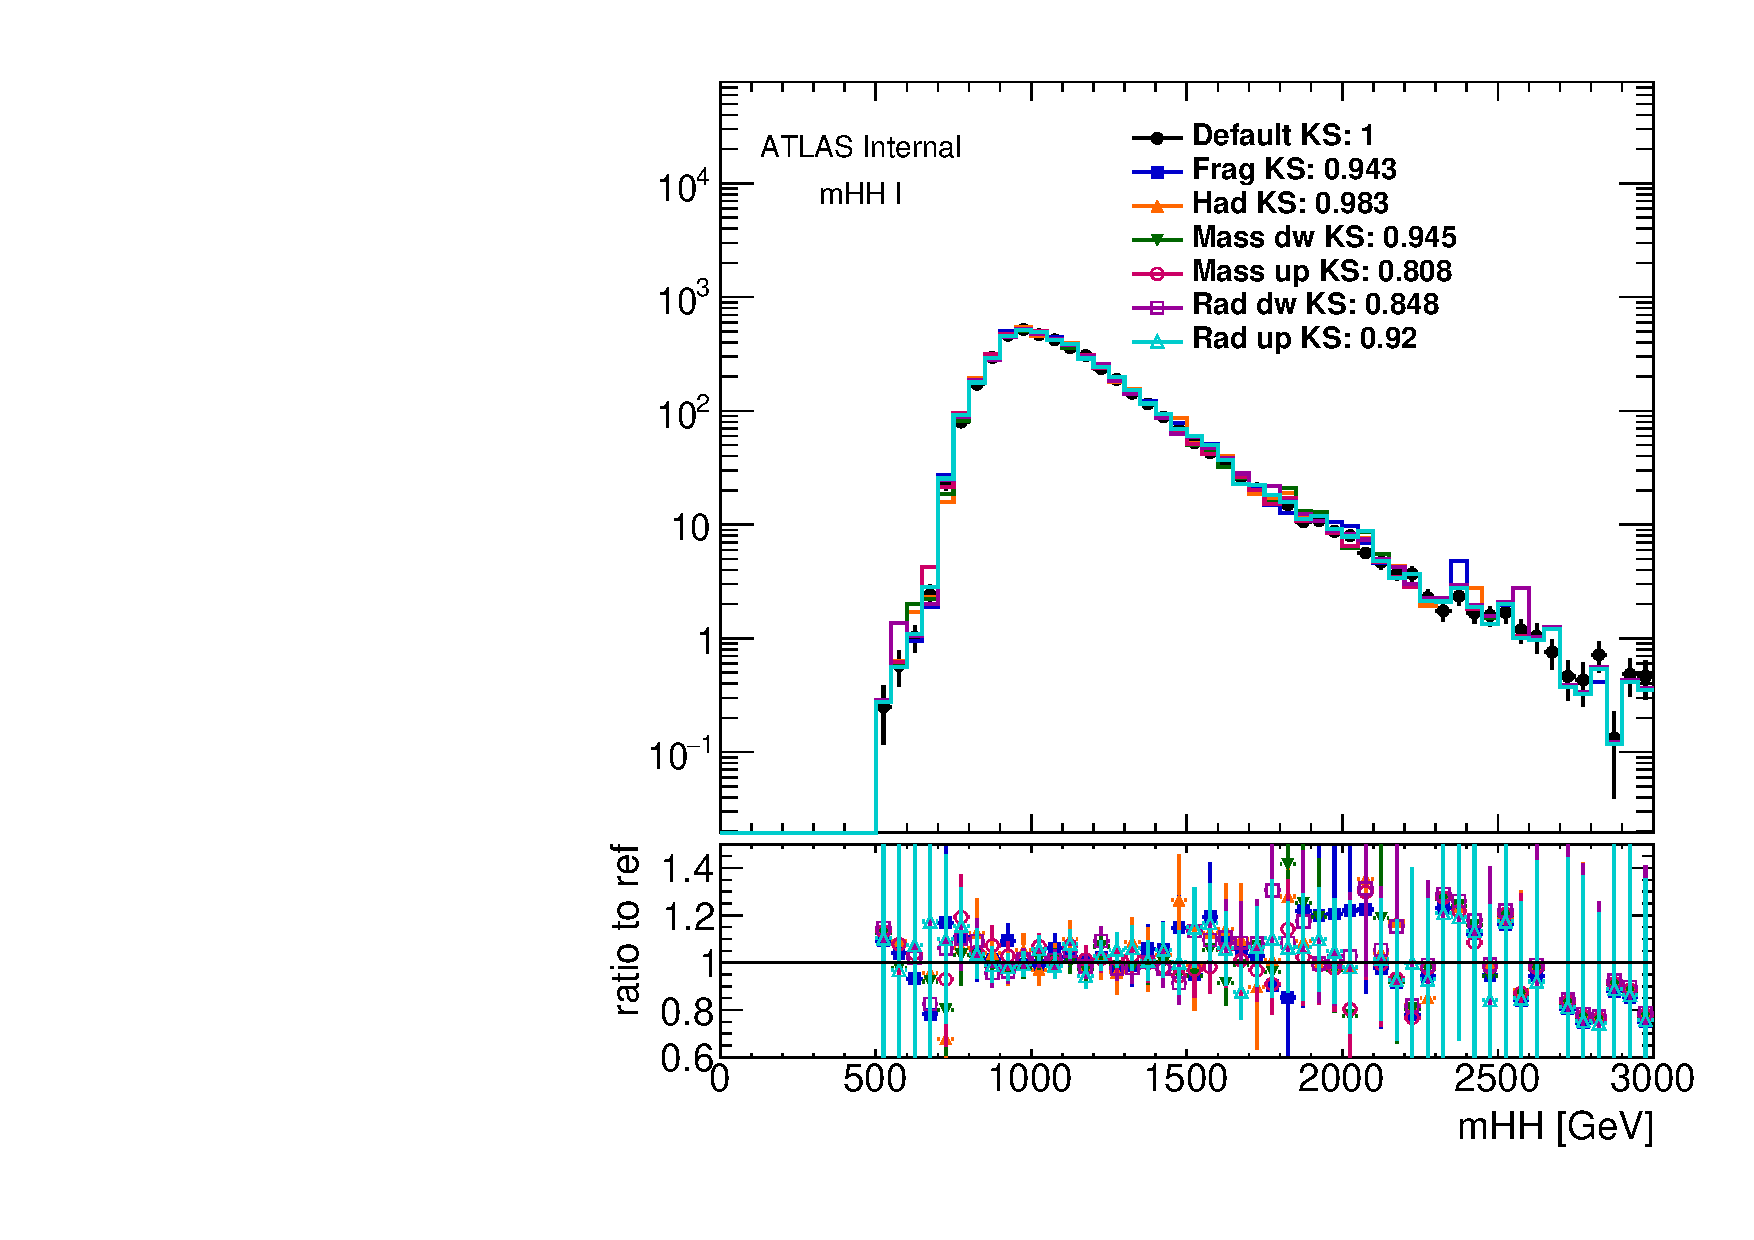
\includegraphics[width=0.48\textwidth,angle=-90]{figures/boosted/Other/directcompare_mHH_l_1_TwoTag_split_Top_syst_stat_postfit_all_.pdf}
\caption{Total background estimation (qcd + \ttbar) with different \ttbar MC variations. The different variations agree with the default within the statistical uncertainties.}
\label{fig:ttbar-MC}
\end{center}
\end{figure}

%%%%%%%%%%%%%%%%%%%%%%%%%%%%%%%%%%%%%%%%%%%%%%%%%%%%%%%%%%%%%%%%%%%%%%%
%%%%%%%%%%%%%%%%%%%%%%%%%%%%%%%%%%%%%%%%%%%%%%%%%%%%%%%%%%%%%%%%%%%%%%%
\section{Theoretical uncertainties}
\label{sec:boosted-systematics-theory}
\paragraph{}
The theoretical uncertainties on the acceptance times efficiency ($A\times\varepsilon$) are evaluated by analysis of specially-generated, particle-level signal samples. 
The generation of these samples follows the configuration of the baseline samples, but with modifications to probe the following theoretical uncertainties: uncertainties in the parton density functions; uncertainties due to missing higher order terms in the matrix elements; and uncertainties in the modelling of the underlying event (including multi-parton interactions), of hadronic showers and of initial and final state radiation. Each of the signals is tested.

\paragraph{}
The estimation of the theoretical uncertainties is performed using a Rivet-based analysis, which replicates the full analysis selection outlined in Section \ref{sec:selection}. The most important detector effects -- b-tagging efficiency and jet mass resolution -- are emulated. Jet mass resolution is emulated by smearing the particle-level $R=1.0$ jet masses, using the resolutions estimated in \cite{ATLAS-CONF-2016-035}. B-tagging efficiency is treated using a truth-tagging approach, which weights events according to the combinatoric probabilities of which jets are b-tagged, using the measured b-tagging efficiencies from the CDI file. 

\paragraph{}
Reasonable agreement is observed between the acceptance times efficiency of the particle-level analysis and of the full, reconstruction-level analysis when measured on independent samples generated using the same configuration, although there are clearly discrepancies. Perfect agreement is not necessary, since the theoretical uncertainties will be calculated using the relative change in $A\times\varepsilon$ between variations of the signal sample, as measured by the Rivet-based analysis.

\paragraph{}
To evaluate the potential effect of missing higher order terms in the matrix element, the renormalisation and factorisation scales used in the signal generation were varied coherently by factors of $0.5\times$ and $2\times$ for the signals. 

\paragraph{}
Uncertainties due to modelling of the parton shower and the underlying event (including multi-parton interactions) are evaluated by switching the MC generator used. For the Bulk RS graviton samples, this means switching from Pythia 8 to Herwig++, while for the scalar and non-resonant it is Herwig++ to Pythia 8.

\paragraph{}
PDF uncertainties are evaluated using the PDF4LHC15\_nlo\_mc set, which combines CT14, MMHT14 and NNPDF3.0 PDF sets \cite{0954-3899-43-2-023001}. The uncertainty is evaluated by calculating the acceptance for each PDF replica. The standard deviation of these acceptance values divided by the baseline acceptance is taken as the PDF uncertainty. For each mass point the distribution of these ratio is compatible with a Gaussian centred on one. 
The uncertainty in acceptance due to PDF uncertainties is less than $\pm1\%$ across the full mass range considered for the analysis. For this reason, it is neglected in the statistical analysis described in Section \ref{sec:statistical-analysis}.

\paragraph{}
These uncertainties are implemented in the final statistical analysis as normalisation uncertainties on the signals, with the value taken from the polynomial fit. 
This smooths out statistical fluctuations and allows interpolation between the generated mass points, if needed.


%%%%%%%%%%%%%%%%%%%%%%%%%%%%%%%%%%%%%%%%%%%%%%%%%%%%%%%%%%%%%%%%%%%%%%%
%%%%%%%%%%%%%%%%%%%%%%%%%%%%%%%%%%%%%%%%%%%%%%%%%%%%%%%%%%%%%%%%%%%%%%%

\subsection{Background prediction uncertainty}
\label{sec:boosted-systematics-bkg}

\paragraph{}
A statistical uncertainty on the value of \muqcd for the $4b$ ($3b$, $2bs$) Signal Region was determined from the fitting procedure described in Section~\ref{sec:ttbarnorm}.

\paragraph{}
The statistical uncertainty of the \ttbar\ normalization is accounted for through the uncertainties on \alphatt from the fit to data, as described in Section~\ref{sec:ttbarnorm}. The statistical uncertainty of 69\% on \alphatt are 79\% anti-correlated to the value of \muqcd found in the fitting procedure in the 4 $b$-tag region, the uncertainties of 9\% on \alphatt are 76\% anti-correlated to the value of \muqcd found in the fitting procedure in the 3 $b$-tag region, and the uncertainties of 2.6\% on \alphatt are 75\% anti-correlated to the value of \muqcd found in the fitting procedure in the $2bs$-tag region.

\paragraph{}
The background systematic uncertainties in the signal region are divided into the following components:
\begin{itemize}
 \item Non-closure uncertainty on \muqcd found by comparing the value derived from the sideband to the control region normalization.
 \item Effects on the QCD prediction from variations of the SideBand and Control Region Definitions
 \item The impact of the shape uncertainty of the \ttbar\ distribution in the $4b$ signal region.
 \item The impact of the shape uncertainty of the 1/$2b$ QCD distribution derived in the control region.
 \item The impact of the smoothing function fit range and function choice on the QCD prediction
\end{itemize}

\paragraph{}
The \ttbar\ normalization uncertainty on \alphatt is derived in the fit to data as described in Section~\ref{sec:ttbarnorm}. This has a negligible impact on the signal sensitivity, but is still propagated as the uncertainty in the \ttbar\ normalization in the signal region.
However, the \ttbar\ background estimation can impact the value of $\mu_{QCD}$ used to determine the QCD normalization in the signal region, where a 53\% (60\%) correlation was found in the fitting procedure between \muqcd and \alphatt in the 4 (3) $b$-tag region This and the other background uncertainty components will be discussed in this section. 

\subsection{Non-closure uncertainty on \muqcd determined in the control region}
\label{sec:non-closure-mu-qcd}

\paragraph{}
A further uncertainty is derived by comparing the value of \muqcd to the overall difference between predicted to observed events in the control region. While the total predicted background (showing stat error only) of $4b$: 76.7 $\pm$ 5.4 vs obs 81.0, $3b$: 1565.6 $\pm$ 18.1 vs obs 1553.0, $2bs$: 8332.4 $\pm$ 38.8 vs obs 8486.0, the number events agrees with the total data in the control region within statistical error, we consider an added systematic on the background prediction normalization, taken a as the maximum between either the difference between the central value of the prediction to the observed number of events (4.3 events, or 5\%, for $4b$.  13 events, or 1\%, for $3b$; 154 events, or 2\%, for $2bs$) or the statistical uncertainty of the observed 4b (3b) data in the CR (11.1\% for $4b$; 2.5\% for $3b$; and 1.1\% for $2bs$). For the detailed numbers, please refer to section ~\ref{sec:yields}. 

\paragraph{}
Although we have derived our non-closure uncertainty on $\mu_{QCD}$ from comparison between data and prediction in the control region, we need to test how this number is sensitive to our choice of control region (CR) and sideband region (SB). In addition, we also want to check how our background prediction in signal region is sensitive to the choice of control region and sideband region. All these tests are done on the control/sideband regions after the full reweighting procedure as described in \ref{sec:boosted-reweight}, while applying the nominal reweighting values.

\paragraph{}
Besides the nominal control region as described above, we design three additional control regions, as illustrated in Figure \ref{CRSB:CR_High}, \ref{CRSB:CR_Low}, \ref{CRSB:CR_Small}, \ref{CRSB:SB_High}, \ref{CRSB:SB_Low}, \ref{CRSB:SB_Large}, \ref{CRSB:SB_Small}:
\begin{itemize}
	\item Low-mass CR: the center position of the circle that defines nominal CR is moved down by 3 GeV, in both leading and sub-leading large-jet mass.
	\item High-mass CR: the center position of the circle that defines nominal CR is moved up by 3 GeV, in both leading and sub-leading large-R jet mass.
	\item Signal-depletion (Small) CR: the $X_{hh}$ cut that defines signal region is increased to $2.0$ from $1.6$. This variation only affect CR, while SR remains unchanged (i.e. signal region is still defined by $X_{hh}<1.6$, while CR is defined as $X_{hh}>2.0$ and $R_{hh}<33$).
	\item High-mass SB: The signal region and control region remain unchanged, the center position of the circle that defines nominal SB is moved up by 3 GeV in both leading and sub-leading large-R jet mass.
	\item Low-mass SB: The signal region and control region remain unchanged, the center position of the circle that defines nominal SB is moved up by 3 GeV in both leading and sub-leading large-R jet mass.
	\item Large SB: The signal region and control region remain unchanged, while the SB is $33 < R_{hh}$ and $ R_{hh}^{\text{high}} < 61$. $\mu_{QCD}$ will change.
	\item Small SB: The signal region and control region remain unchanged, while the SB is $33 < R_{hh}$ and $ R_{hh}^{\text{high}} < 55$. $\mu_{QCD}$ will change.
\end{itemize}

\paragraph{}
To ensure that these value cover the QCD normalization uncertainty, further checks on the effect of adjusting the Control and Sideband definitions were done. 
The results are summarized in Table \ref{CRSB:Tab_4b_CR_Variations}, \ref{CRSB:Tab_3b_CR_Variations} and \ref{CRSB:Tab_2bs_CR_Variations}, while the details are presented in the Appendix~\ref{app:boosted-syst-CRSB_Definition_Variation}. Based on all the variations, a 2.8\% normalization uncertainty is assigned to $2bs$ region, 4.2\% to $3b$ region (which is the statistical uncertainty), and a 12.2\% normalization uncertainty is assigned to $4b$ region.

\begin{table}[htbp!]
\begin{center}
\begin{footnotesize} 
\begin{tabular}{c|c|c|c} 
CR Varations FourTag & Data & Prediction & (Predict - Data)/Data \\ 
\hline\hline 
& & & \\ 
Nominal & 81.0 $\pm$ 9.0 & 76.77 $\pm$ 5.43 & -5.22 $\%$  $\pm$ 17.23 $\%$ \\ 
\hline 
CR High & 76.0 $\pm$ 8.72 & 71.12 $\pm$ 5.41 & -6.43 $\%$  $\pm$ 17.85 $\%$ \\ 
\hline 
CR Low & 91.0 $\pm$ 9.54 & 79.87 $\pm$ 5.45 & -12.2 $\%$  $\pm$ 15.19 $\%$ \\ 
\hline 
CR Small & 58.0 $\pm$ 7.62 & 55.96 $\pm$ 5.35 & -3.52 $\%$  $\pm$ 21.89 $\%$ \\ 
\hline 
SB Large & 81.0 $\pm$ 9.0 & 74.71 $\pm$ 5.4 & -7.76 $\%$  $\pm$ 16.91 $\%$ \\ 
\hline 
SB Small & 81.0 $\pm$ 9.0 & 74.15 $\pm$ 5.38 & -8.45 $\%$  $\pm$ 16.81 $\%$ \\ 
\hline 
SB High & 81.0 $\pm$ 9.0 & 78.72 $\pm$ 5.46 & -2.82 $\%$  $\pm$ 17.54 $\%$ \\ 
\hline 
SB Low & 81.0 $\pm$ 9.0 & 76.51 $\pm$ 5.38 & -5.54 $\%$  $\pm$ 17.14 $\%$ \\ 
& & & \\ 
\hline\hline 
\end{tabular} 
\end{footnotesize} 
\newline 

\end{center}
\caption{Agreement between data and prediction in 4b tag CR. Showing stat uncertainty only.}
\label{CRSB:Tab_4b_CR_Variations}
\end{table}

\begin{table}[htbp!]
\begin{center}
\begin{footnotesize} 
\begin{tabular}{c|c|c|c} 
CR Varations ThreeTag & Data & Prediction & (Predict - Data)/Data \\ 
\hline\hline 
Nominal & 1553.0 $\pm$ 39.41 & 1587.04 $\pm$ 21.4 & 2.19 $\%$  $\pm$ 3.97 $\%$ \\ 
\hline 
CR High & 1461.0 $\pm$ 38.22 & 1473.89 $\pm$ 20.77 & 0.88 $\%$  $\pm$ 4.06 $\%$ \\ 
\hline 
CR Low & 1628.0 $\pm$ 40.35 & 1697.38 $\pm$ 21.75 & 4.26 $\%$  $\pm$ 3.92 $\%$ \\ 
\hline 
CR Small & 1134.0 $\pm$ 33.67 & 1127.34 $\pm$ 17.66 & -0.59 $\%$  $\pm$ 4.51 $\%$ \\ 
\hline 
SB Large & 1553.0 $\pm$ 39.41 & 1574.23 $\pm$ 21.47 & 1.37 $\%$  $\pm$ 3.95 $\%$ \\ 
\hline 
SB Small & 1553.0 $\pm$ 39.41 & 1601.44 $\pm$ 21.64 & 3.12 $\%$  $\pm$ 4.01 $\%$ \\ 
\hline 
SB High & 1553.0 $\pm$ 39.41 & 1602.74 $\pm$ 21.48 & 3.2 $\%$  $\pm$ 4.0 $\%$ \\ 
\hline 
SB Low & 1553.0 $\pm$ 39.41 & 1576.56 $\pm$ 21.5 & 1.52 $\%$  $\pm$ 3.96 $\%$ \\ 
\hline\hline 
\end{tabular} 
\end{footnotesize} 
\newline 

\end{center}
\caption{Agreement between data and prediction in 3b tag CR. Showing stat uncertainty only.}
\label{CRSB:Tab_3b_CR_Variations}
\end{table}
\begin{table}[htbp!]
\begin{center}
\begin{footnotesize} 
\begin{tabular}{c|c|c|c} 
CR Varations TwoTag split & Data & Prediction & (Predict - Data)/Data \\ 
\hline\hline 
& & & \\ 
Nominal & 8486.0 $\pm$ 92.12 & 8332.97 $\pm$ 38.84 & -1.8 $\%$  $\pm$ 1.52 $\%$ \\ 
\hline 
CR High & 8174.0 $\pm$ 90.41 & 7937.59 $\pm$ 39.61 & -2.89 $\%$  $\pm$ 1.56 $\%$ \\ 
\hline 
CR Low & 8907.0 $\pm$ 94.38 & 8800.86 $\pm$ 39.51 & -1.19 $\%$  $\pm$ 1.49 $\%$ \\ 
\hline 
CR Small & 5999.0 $\pm$ 77.45 & 5873.52 $\pm$ 32.31 & -2.09 $\%$  $\pm$ 1.8 $\%$ \\ 
\hline 
SB Large & 8486.0 $\pm$ 92.12 & 8341.7 $\pm$ 38.44 & -1.7 $\%$  $\pm$ 1.52 $\%$ \\ 
\hline 
SB Small & 8486.0 $\pm$ 92.12 & 8333.25 $\pm$ 39.12 & -1.8 $\%$  $\pm$ 1.53 $\%$ \\ 
\hline 
SB High & 8486.0 $\pm$ 92.12 & 8378.14 $\pm$ 38.45 & -1.27 $\%$  $\pm$ 1.52 $\%$ \\ 
\hline 
SB Low & 8486.0 $\pm$ 92.12 & 8356.86 $\pm$ 39.06 & -1.52 $\%$  $\pm$ 1.53 $\%$ \\ 
& & & \\ 
\hline\hline 
\end{tabular} 
\end{footnotesize} 
\newline 

\end{center}
\caption{Agreement between data and prediction in 2bs tag CR. Showing stat uncertainty only.}
\label{CRSB:Tab_2bs_CR_Variations}
\end{table}


\clearpage
\subsection{Validation of background estimation from low mass and high mass signal region}
\label{sec:boosted-ZZ-Rehearsal}
\paragraph{}
Another check is the the so-called "low mass signal region rehearsal" (or ZZ region) and "high mass signal region rehearsal" (or TT region). Instead of a signal region around di-Higgs mass region on leading-subleading large-R jet mass 2D plane, we redefine a separate lower mass (ZZ) and higher mass (TT) signal region: 
\begin{equation}
X_{ZZ} = \sqrt{\left(\frac{m(J_1) - \text{103 GeV}}{0.1 m(J_1)}\right)^2 + \left(\frac{m(J_2) - \text{96 GeV}}{0.1 m(J_2)}\right)^2} < 1.6 
\label{eq:boosted_Xzz}
\end{equation}
\begin{equation}
X_{TT} = \sqrt{\left(\frac{m(J_1) - \text{164 GeV}}{0.1 m(J_1)}\right)^2 + \left(\frac{m(J_2) - \text{155 GeV}}{0.1 m(J_2)}\right)^2} < 1.6
\label{eq:boosted_Xtt}
\end{equation}
which is also illustrated in Figure \ref{CRSB:ZZIllustration}. The analysis is repeated, using the same definition of Sideband and Control region as nominal (but with events contained in ZZ signal region excluded) for normalization fit. Then the low mass signal region is unblinded. This helps to validate the background estimation strategy, and the stability for other similar analysis.

\begin{figure}[htbp!]
\begin{center}
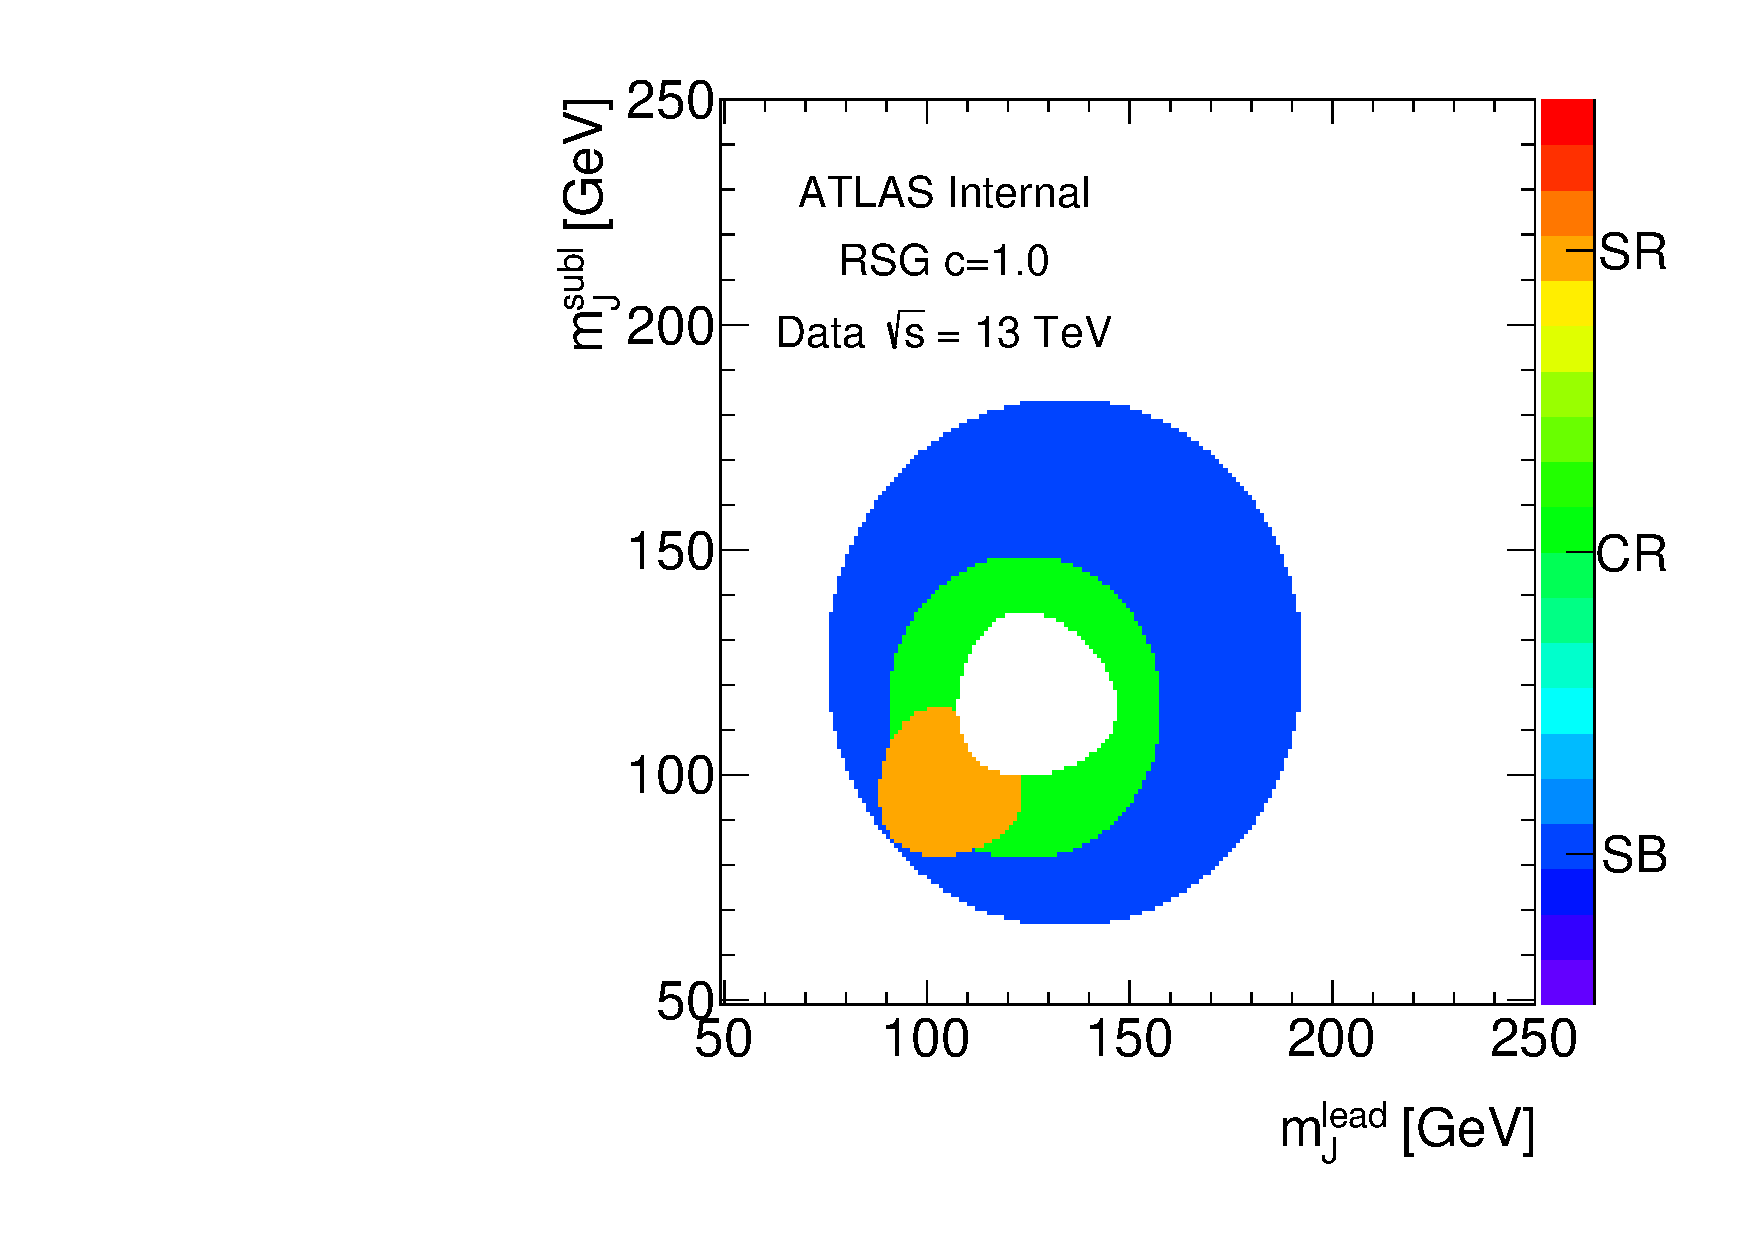
\includegraphics[width=0.4\textwidth,angle=-90]{figures/boosted/ZZ/Compare_NoTag_mH0H1.pdf}
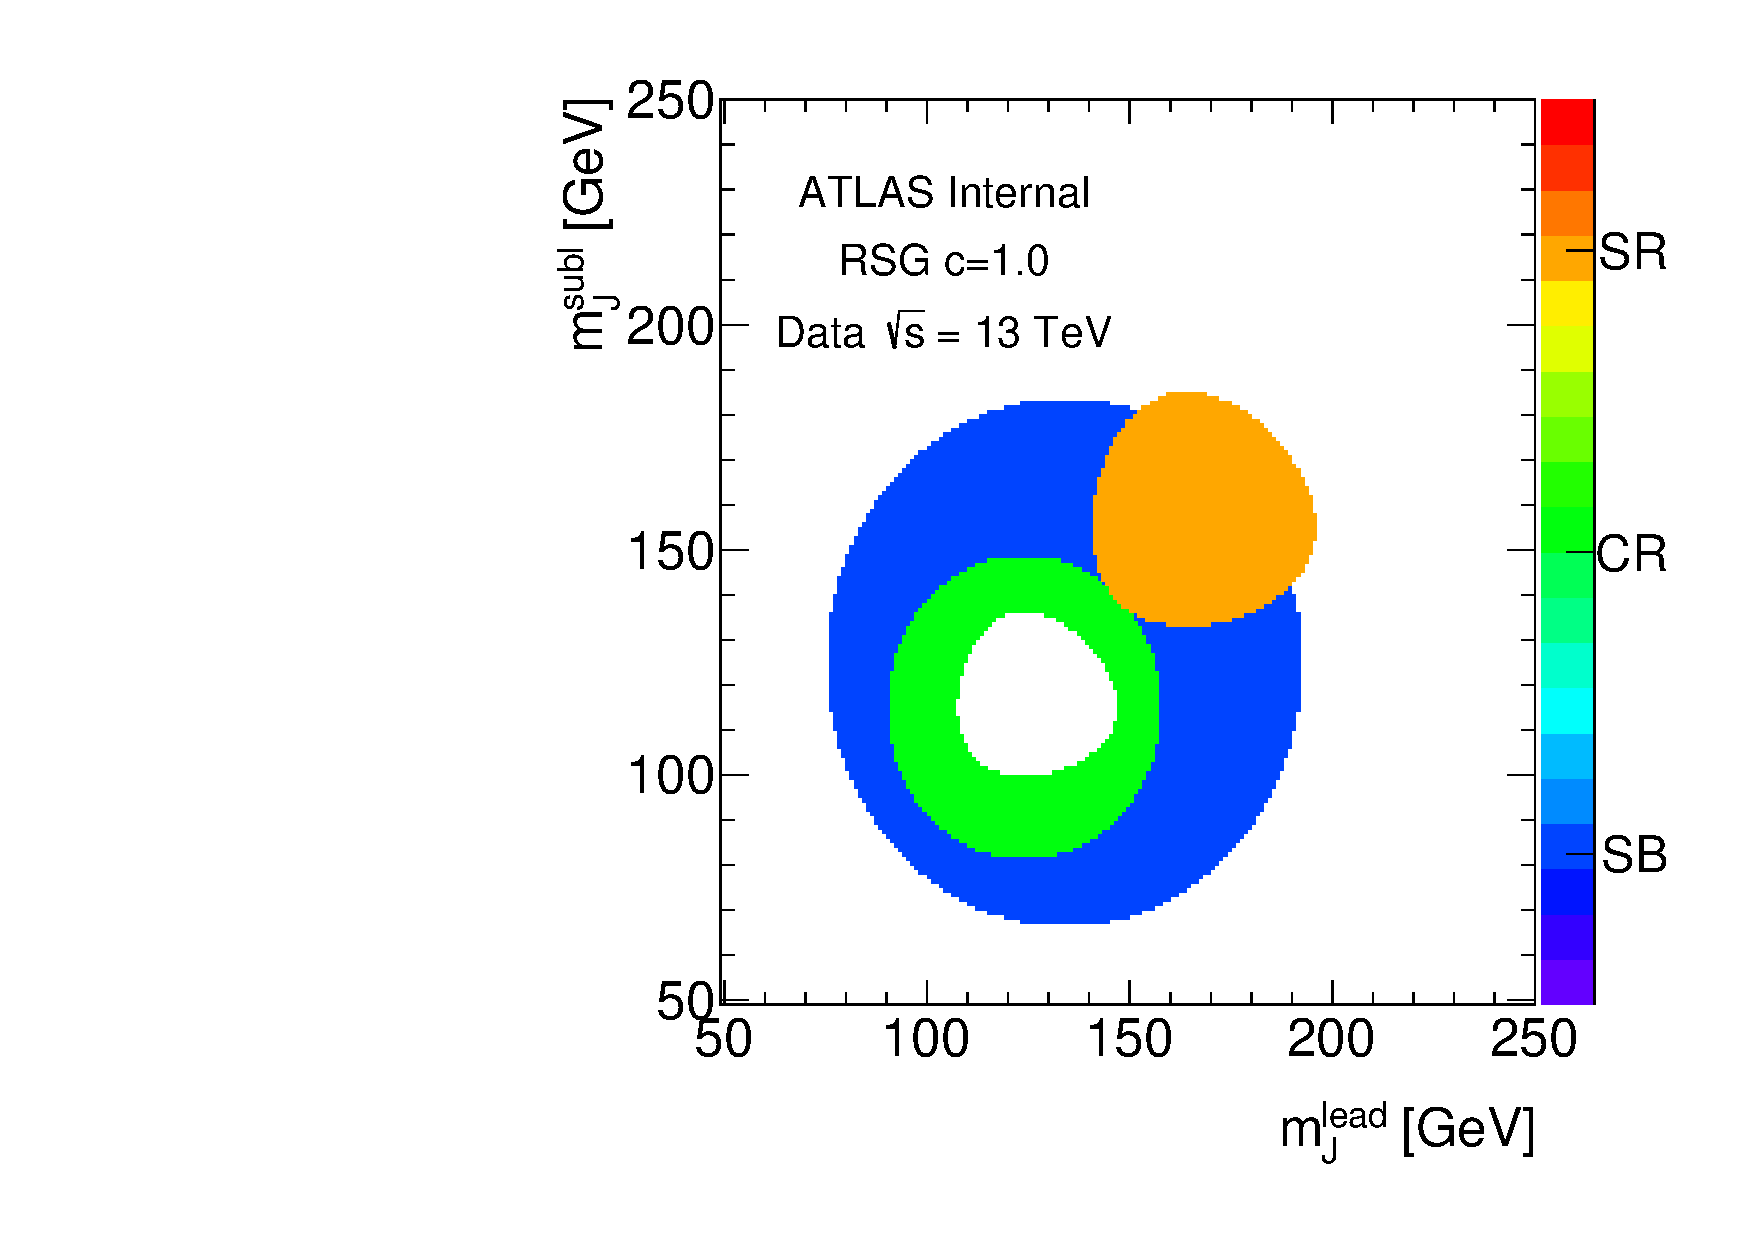
\includegraphics[width=0.4\textwidth,angle=-90]{figures/boosted/TT/Compare_NoTag_mH0H1.pdf}
\end{center}
\caption{Illustration of ZZ (left) and TT (right) signal region as shown in the orange shaded region. Control region shown in green, and Sideband region in blue. The white circle in the midde is the real Signal region, and it is blinded.}
\label{CRSB:ZZIllustration}
\end{figure}

\paragraph{}
The summary of background estimation for ZZ signal region can be found in Table \ref{CRSB:SummaryTable_ZZ_4b}, ~\ref{CRSB:SummaryTable_ZZ_3b} and ~\ref{CRSB:SummaryTable_ZZ_2b}. The difference between data and prediction in ZZ signal region is summarized in Table \ref{CRSB:DataPred_ZZSR} for all the regions. The discrepancy between data and prediction is either covered by statistical uncertainty of data or comparable with data statistical uncertainty in $4b$, $3b$ and $2bs$ ZZ SR respectively. We further check the kinematic distribution between data and prediction in ZZ SR, as shown in Figure \ref{CRSB:ZZSR_Distribution}. The data agrees with prediction well in general, though a few bins might not agree perfectly. The difference from $4b$ CR region test is 17$\%$, which is smaller than the $4b$ ZZ region difference. But the statistical uncertainty in ZZ region (yield 37) is much higher compared with our CR regions (min yield 76), hence the CR region with more statistical power is still used for the non-closure uncertainty.

\paragraph{}
The summary of background estimation for TT signal region can be found in Table \ref{CRSB:SummaryTable_TT_4b}, ~\ref{CRSB:SummaryTable_TT_3b} and ~\ref{CRSB:SummaryTable_TT_2b}. The difference between data and prediction in TT signal region is summarized in Table \ref{CRSB:DataPred_TTSR} for all the regions. The discrepancy between data and prediction is either covered by statistical uncertainty of data or comparable with data statistical uncertainty in $4b$, $3b$ and $2bs$ TT SR respectively. We further check the kinematic distribution between data and prediction in TT SR, as shown in Figure \ref{CRSB:TTSR_Distribution}. The data agrees with prediction well in general, though a few bins might not agree perfectly. 

\paragraph{}
Based on all the variation tests done above, we think there is no need to introduce extra uncertainty on non-closure systematics since most of the data/prediction disagreements are well covered by the data statistical uncertainty.

\begin{table}[htbp!]
\begin{center}
\begin{footnotesize} 
\begin{tabular}{c|c|c|c} 
FourTag & Sideband & Control & Signal \\ 
\hline\hline 
QCD Est & 166.65 $\pm$ 2.88 & 45.83 $\pm$ 1.51 & 27.37 $\pm$ 1.16\\ 
$t\bar{t}$ Est.  & 27.52 $\pm$ 0.25 & 6.31 $\pm$ 0.14 & 0 $\pm$ 0\\ 
$Z+jets$ & 0 $\pm$ 0 & 6.18 $\pm$ 5.12 & 0 $\pm$ 0\\ 
Total Bkg Est & 194.17 $\pm$ 2.89 & 58.32 $\pm$ 5.34 & 27.37 $\pm$ 1.16\\ 
Data & 194.0 $\pm$ 13.93 & 54.0 $\pm$ 7.35 & 37.0 $\pm$ 6.08\\ 
$c=1.0$,$m=1.0TeV$ & 2.45 $\pm$ 0.098 & 4.47 $\pm$ 0.13 & 0.99 $\pm$ 0.063\\ 
$c=1.0$,$m=2.0TeV$ & 0.032 $\pm$ 0.0015 & 0.075 $\pm$ 0.0022 & 0.028 $\pm$ 0.0014\\ 
$c=1.0$,$m=3.0TeV$ & 0.00029 $\pm$ 3.5e-05 & 0.00064 $\pm$ 5e-05 & 0.0002 $\pm$ 2.7e-05\\ 
\hline\hline 
\end{tabular} 
\end{footnotesize} 
\newline 

\end{center}
\caption{Background prediction in SR/CR/SB for ZZ SR in $4b$-tag region. Uncertainties are stat only.}
\label{CRSB:SummaryTable_ZZ_4b}
\end{table}

\begin{table}[htbp!]
\begin{center}
\begin{footnotesize} 
\begin{tabular}{c|c|c|c} 
ThreeTag & Sideband & Control & Signal \\ 
\hline\hline 
& & & \\ 
QCD Est & 3344.46 $\pm$ 26.85 & 998.41 $\pm$ 14.63 & 637.78 $\pm$ 11.87\\ 
$t\bar{t}$ Est.  & 826.66 $\pm$ 25.11 & 136.58 $\pm$ 10.23 & 30.07 $\pm$ 1.24\\ 
$Z+jets$ & 32.49 $\pm$ 11.34 & 8.22 $\pm$ 5.29 & 3.3 $\pm$ 2.0\\ 
Total Bkg Est & 4203.61 $\pm$ 38.47 & 1143.2 $\pm$ 18.62 & 671.15 $\pm$ 12.11\\ 
Data & 4203.0 $\pm$ 64.83 & 1108.0 $\pm$ 33.29 & 645.0 $\pm$ 25.4\\ 
$c=1.0$,$m=1.0TeV$ & 7.56 $\pm$ 0.18 & 9.84 $\pm$ 0.2 & 3.05 $\pm$ 0.11\\ 
$c=1.0$,$m=2.0TeV$ & 0.15 $\pm$ 0.0033 & 0.27 $\pm$ 0.0046 & 0.12 $\pm$ 0.003\\ 
$c=1.0$,$m=3.0TeV$ & 0.0034 $\pm$ 0.00012 & 0.0056 $\pm$ 0.00016 & 0.0021 $\pm$ 9.5e-05\\ 
& & & \\ 
\hline\hline 
\end{tabular} 
\end{footnotesize} 
\newline 

\end{center}
\caption{Background prediction in SR/CR/SB for ZZ SR in $3b$-tag region. Uncertainties are stat only.}
\label{CRSB:SummaryTable_ZZ_3b}
\end{table}

\begin{table}[htbp!]
\begin{center}
\begin{footnotesize} 
\begin{tabular}{c|c|c|c} 
TwoTag split & Sideband & Control & Signal \\ 
\hline\hline 
QCD Est & 16387.44 $\pm$ 37.6 & 4827.76 $\pm$ 19.86 & 3026.83 $\pm$ 15.61\\ 
$t\bar{t}$ Est.  & 7671.95 $\pm$ 69.14 & 1229.96 $\pm$ 26.54 & 332.29 $\pm$ 13.66\\ 
$Z+jets$ & 44.37 $\pm$ 13.23 & 13.34 $\pm$ 6.6 & 36.47 $\pm$ 12.88\\ 
Total Bkg Est & 24103.77 $\pm$ 79.8 & 6071.07 $\pm$ 33.8 & 3395.59 $\pm$ 24.42\\ 
Data & 24104.0 $\pm$ 155.25 & 6261.0 $\pm$ 79.13 & 3258.0 $\pm$ 57.08\\ 
$c=1.0$,$m=1.0TeV$ & 4.57 $\pm$ 0.14 & 4.65 $\pm$ 0.14 & 1.91 $\pm$ 0.089\\ 
$c=1.0$,$m=2.0TeV$ & 0.16 $\pm$ 0.0038 & 0.26 $\pm$ 0.0047 & 0.12 $\pm$ 0.0032\\ 
$c=1.0$,$m=3.0TeV$ & 0.012 $\pm$ 0.00024 & 0.019 $\pm$ 0.00029 & 0.0085 $\pm$ 0.00019\\ 
\hline\hline 
\end{tabular} 
\end{footnotesize} 
\newline 

\end{center}
\caption{Background prediction in SR/CR/SB for ZZ SR in $2bs$-tag region. Uncertainties are stat only.}
\label{CRSB:SummaryTable_ZZ_2b}
\end{table}

\begin{table}[htbp!]
\begin{center}
\begin{footnotesize} 
\begin{tabular}{c|c|c|c} 
ZZ Signal Region & Data & Prediction & (Predict - Data)/Data \\ 
\hline\hline 
FourTag & 37.0 $\pm$ 6.08 & 27.37 $\pm$ 1.16 & -26.0 $\%$  $\pm$ 15.3 $\%$ \\ 
\hline 
ThreeTag & 645.0 $\pm$ 25.4 & 671.15 $\pm$ 12.11 & 4.05 $\%$  $\pm$ 5.97 $\%$ \\ 
\hline 
TwoTag split & 3258.0 $\pm$ 57.08 & 3395.59 $\pm$ 24.42 & 4.22 $\%$  $\pm$ 2.58 $\%$ \\ 
\hline\hline 
\end{tabular} 
\end{footnotesize} 
\newline 

\end{center}
\caption{Agreement between data and prediction in ZZ SR in $4b$, $3b$ and $2bs$ regions.}
\label{CRSB:DataPred_ZZSR}
\end{table}

\begin{figure}[htbp!]
\begin{center}
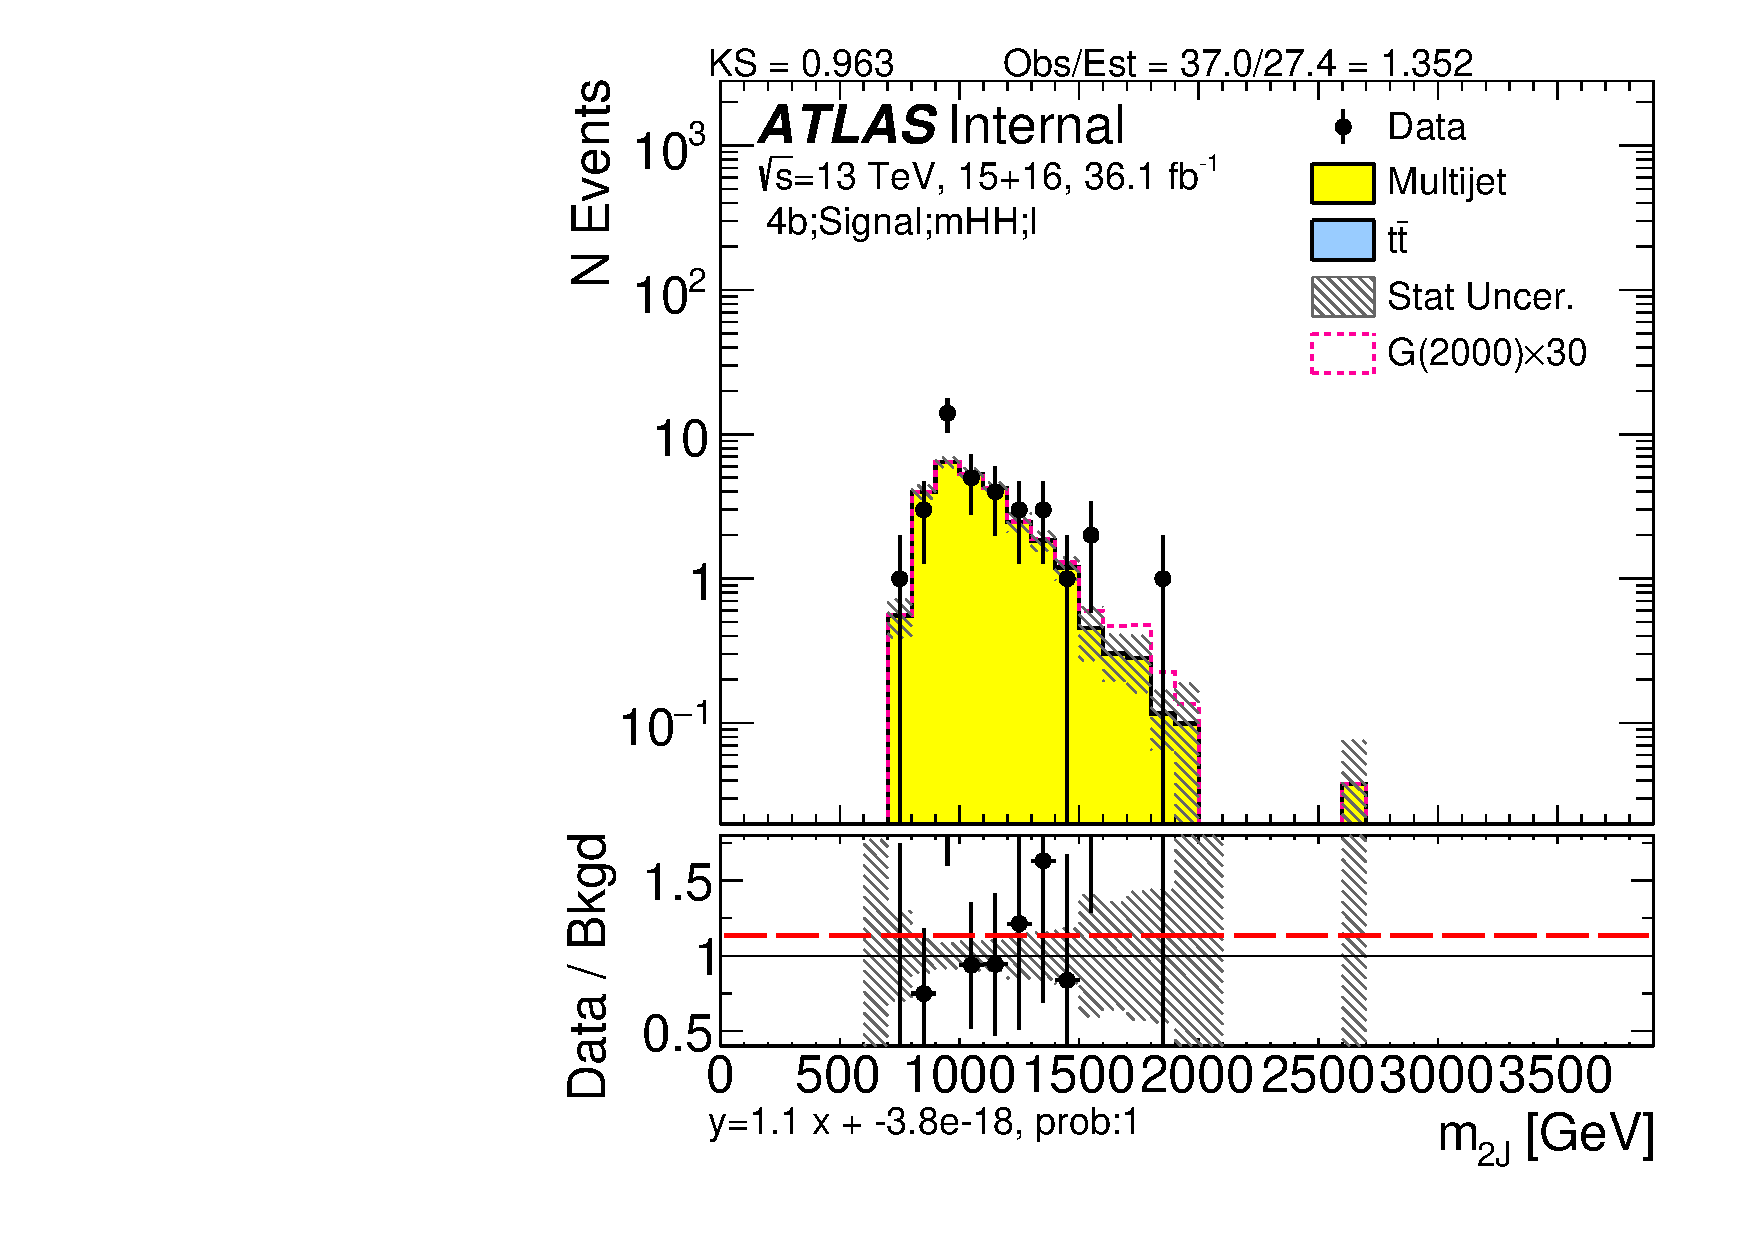
\includegraphics[width=0.45\textwidth,angle=-90]{figures/boosted/ZZ/Moriond_ZZ_FourTag_Signal_mHH_l_1.pdf}
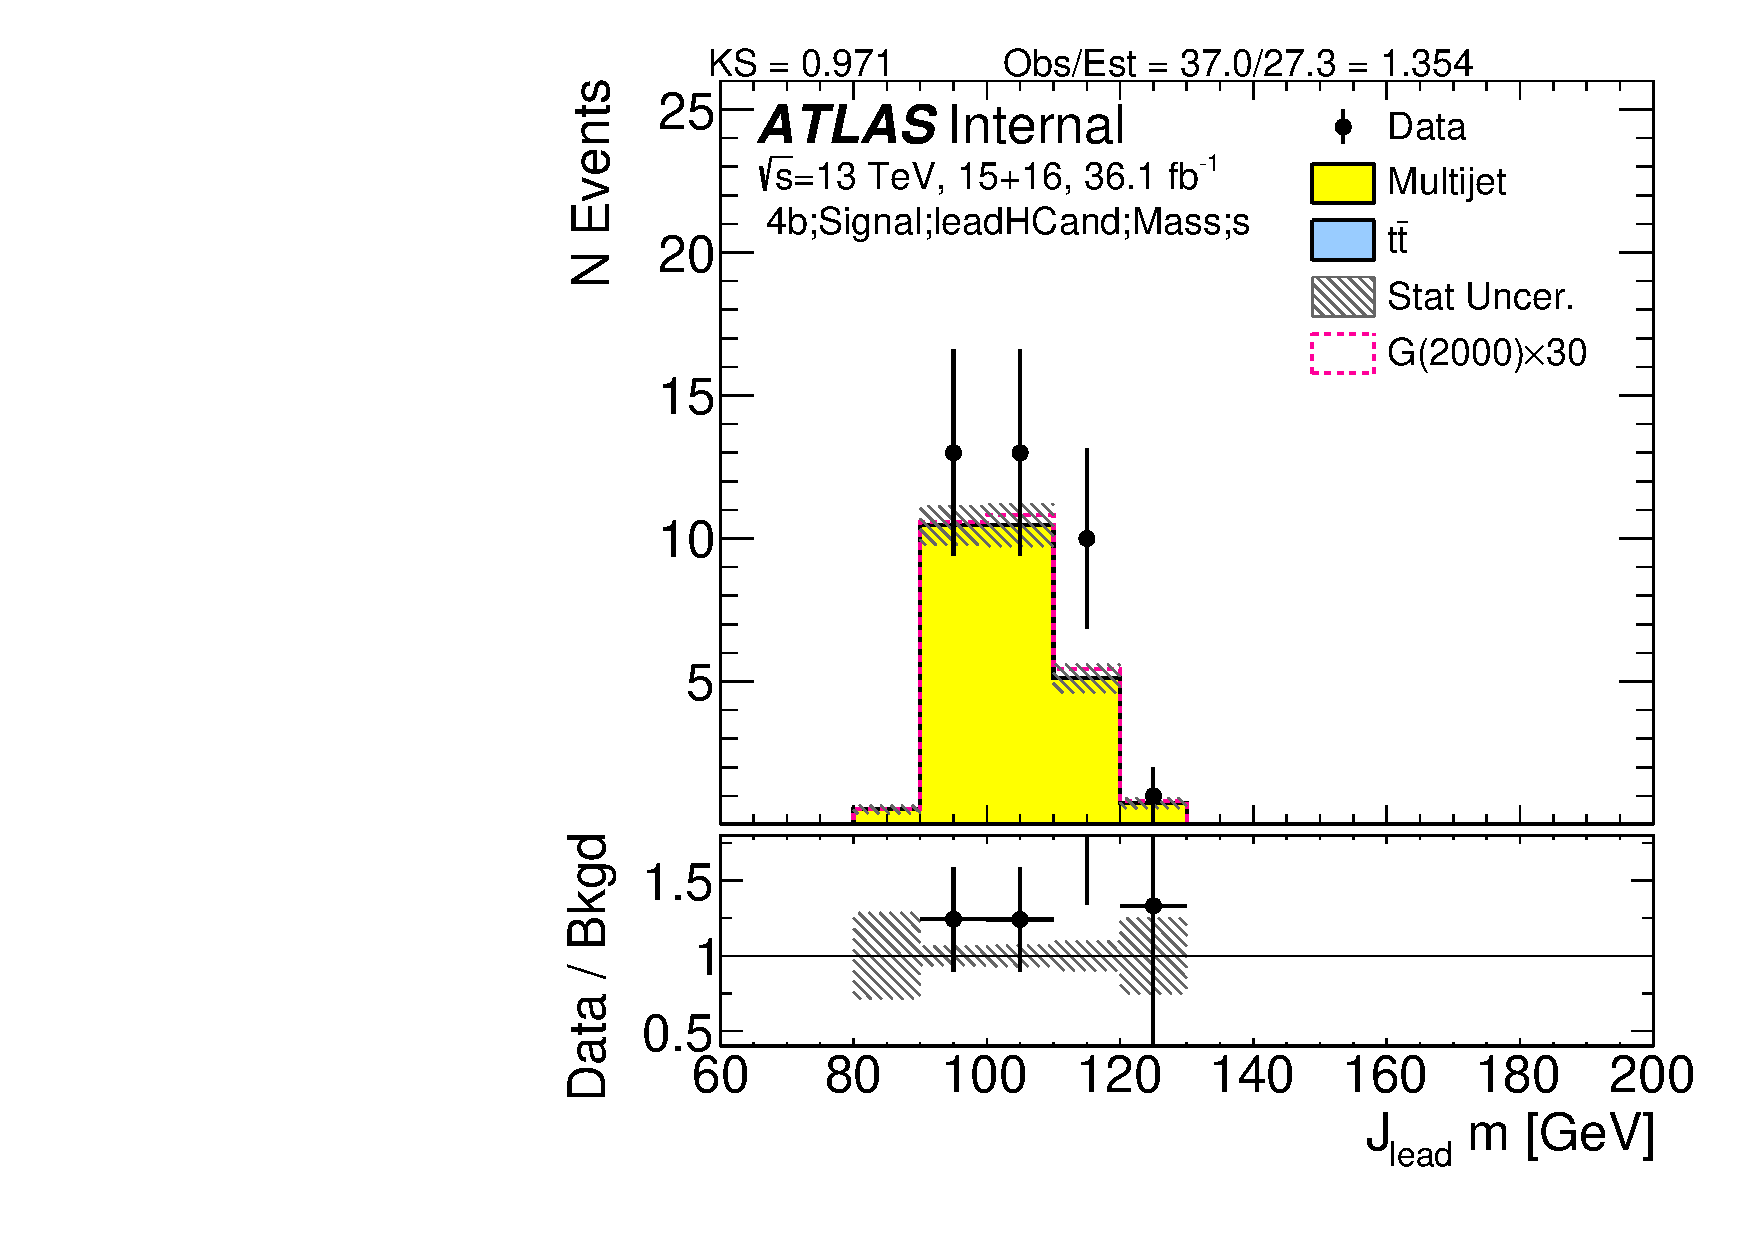
\includegraphics[width=0.45\textwidth,angle=-90]{figures/boosted/ZZ/Moriond_ZZ_FourTag_Signal_leadHCand_Mass_s.pdf}\\
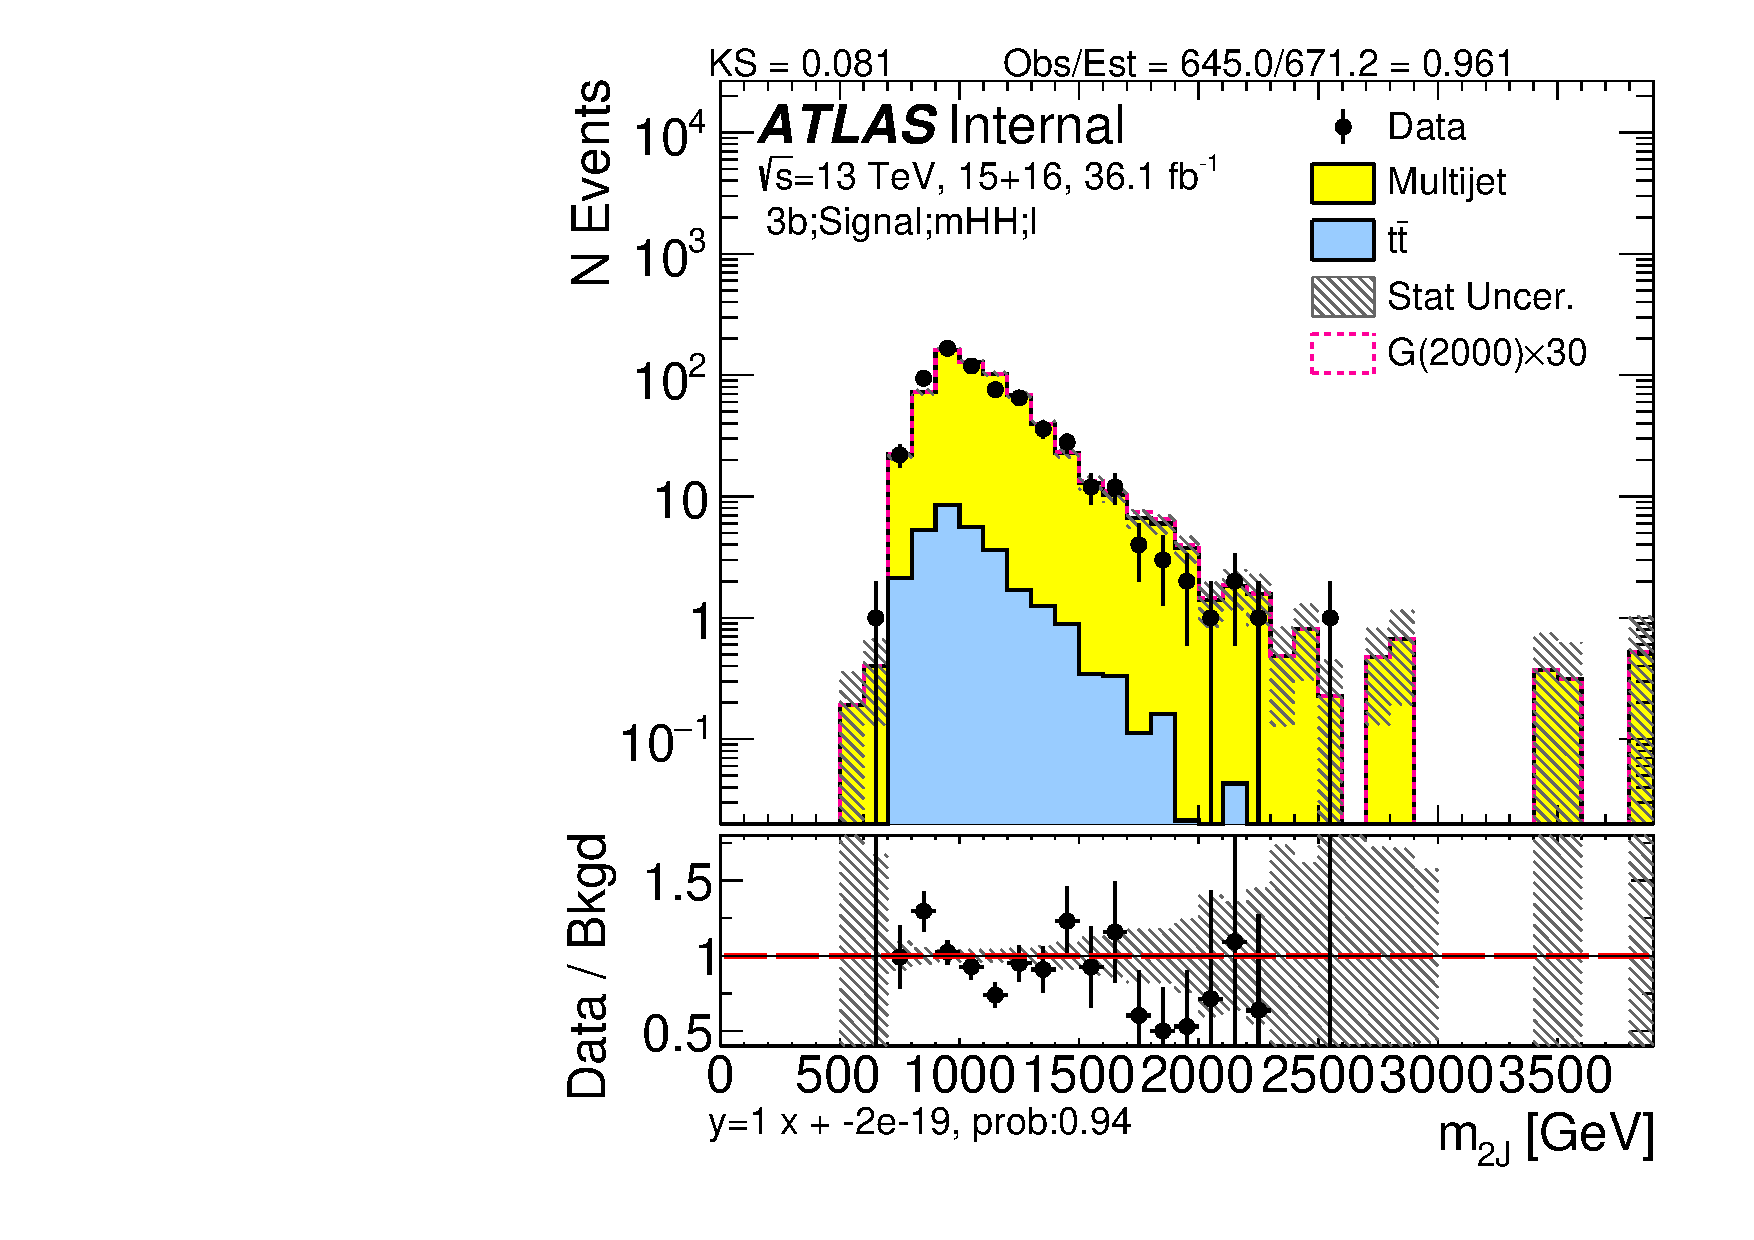
\includegraphics[width=0.45\textwidth,angle=-90]{figures/boosted/ZZ/Moriond_ZZ_ThreeTag_Signal_mHH_l_1.pdf}
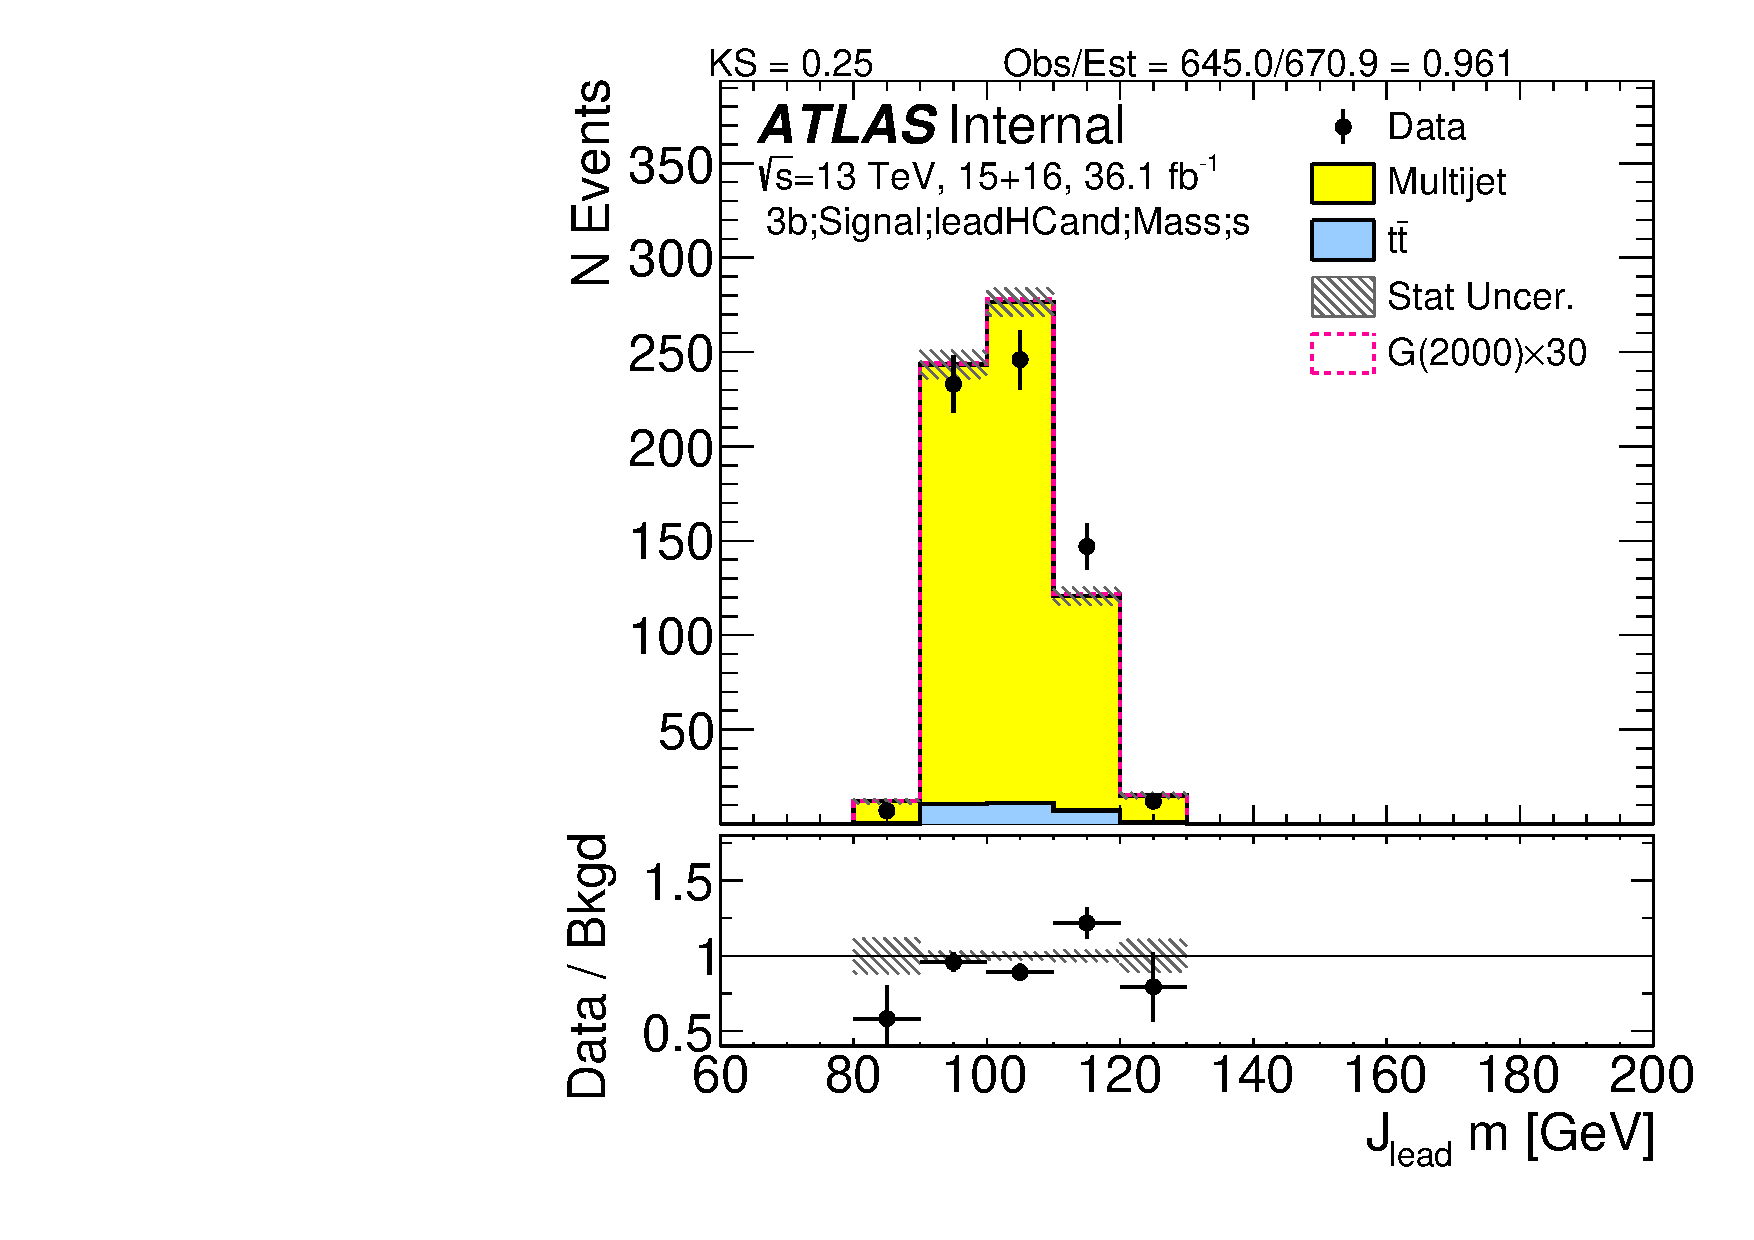
\includegraphics[width=0.45\textwidth,angle=-90]{figures/boosted/ZZ/Moriond_ZZ_ThreeTag_Signal_leadHCand_Mass_s.pdf}\\
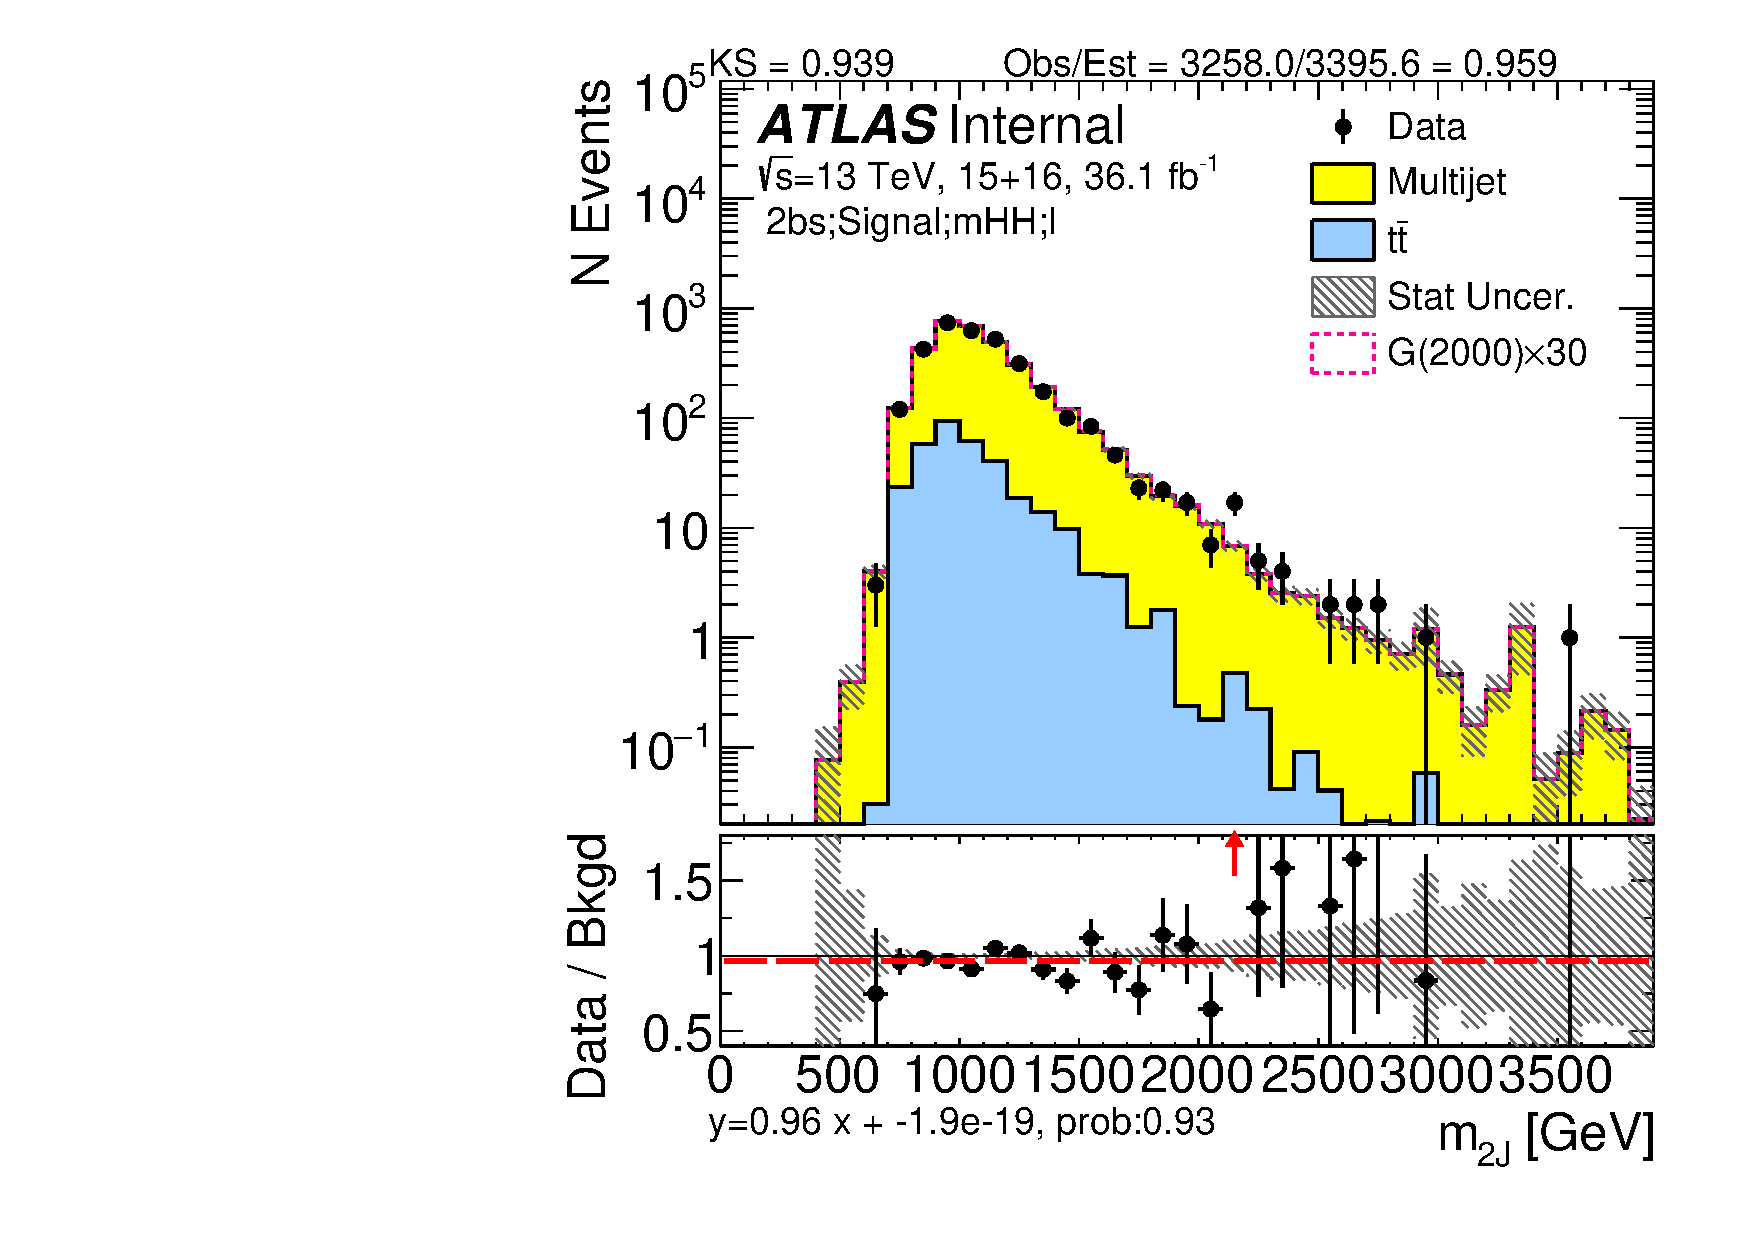
\includegraphics[width=0.45\textwidth,angle=-90]{figures/boosted/ZZ/Moriond_ZZ_TwoTag_split_Signal_mHH_l_1.pdf}
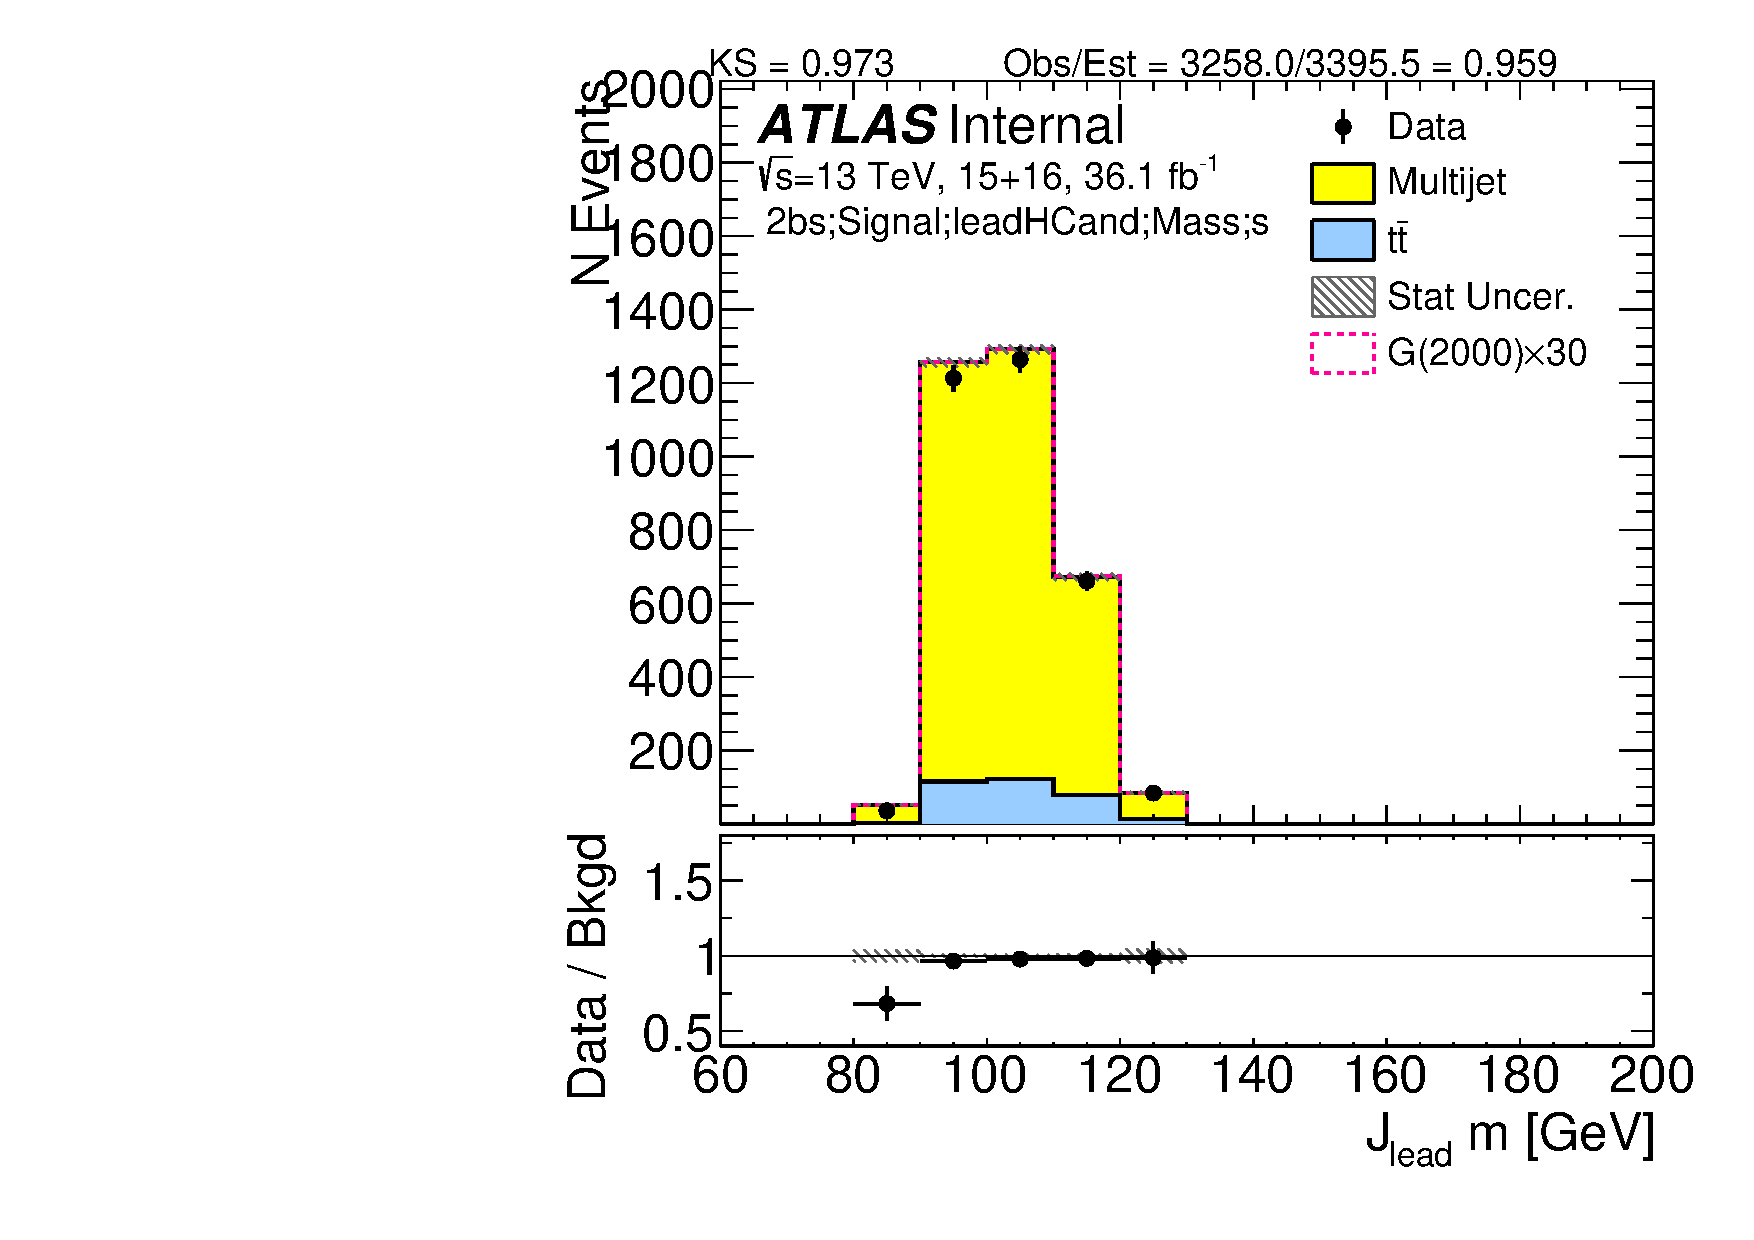
\includegraphics[width=0.45\textwidth,angle=-90]{figures/boosted/ZZ/Moriond_ZZ_TwoTag_split_Signal_leadHCand_Mass_s.pdf}\\
\end{center}
\caption{ZZ signal region distribution of di-jet mass (left column) and leading large-R jet mass (right column) in low mass signal, for $4b$ (top row), $3b$(middle row) and $2b$ split (bottom row). The plots are with only statistical uncertainty.}
\label{CRSB:ZZSR_Distribution}
\end{figure}

\begin{table}[htbp!]
\begin{center}
\begin{footnotesize} 
\begin{tabular}{c|c|c|c} 
FourTag & Sideband & Control & Signal \\ 
\hline\hline 
& & & \\ 
QCD Est & 152.28 $\pm$ 2.72 & 63.47 $\pm$ 1.77 & 28.6 $\pm$ 1.21\\ 
$t\bar{t}$ Est.  & 19.86 $\pm$ 0.22 & 7.45 $\pm$ 0.15 & 15.02 $\pm$ 0.2\\ 
$Z+jets$ & 0 $\pm$ 0 & 6.18 $\pm$ 5.12 & 0 $\pm$ 0\\ 
Total Bkg Est & 172.14 $\pm$ 2.73 & 77.1 $\pm$ 5.42 & 43.62 $\pm$ 1.23\\ 
Data & 172.0 $\pm$ 13.11 & 81.0 $\pm$ 9.0 & 46.0 $\pm$ 6.78\\ 
$c=1.0$,$m=1.0TeV$ & 2.38 $\pm$ 0.097 & 5.4 $\pm$ 0.15 & 0.15 $\pm$ 0.024\\ 
$c=1.0$,$m=2.0TeV$ & 0.033 $\pm$ 0.0015 & 0.1 $\pm$ 0.0026 & 0.0011 $\pm$ 0.00027\\ 
$c=1.0$,$m=3.0TeV$ & 0.00031 $\pm$ 3.6e-05 & 0.0008 $\pm$ 5.6e-05 & 1.5e-05 $\pm$ 7.7e-06\\ 
& & & \\ 
\hline\hline 
\end{tabular} 
\end{footnotesize} 
\newline 

\end{center}
\caption{Background prediction in SR/CR/SB for TT SR in $4b$-tag region. Uncertainties are stat only.}
\label{CRSB:SummaryTable_TT_4b}
\end{table}

\begin{table}[htbp!]
\begin{center}
\begin{footnotesize} 
\begin{tabular}{c|c|c|c} 
ThreeTag & Sideband & Control & Signal \\ 
\hline\hline 
QCD Est & 3106.11 $\pm$ 25.79 & 1427.41 $\pm$ 17.53 & 570.01 $\pm$ 11.6\\ 
$t\bar{t}$ Est.  & 495.21 $\pm$ 18.75 & 148.55 $\pm$ 10.21 & 406.57 $\pm$ 5.42\\ 
$Z+jets$ & 32.5 $\pm$ 11.34 & 11.21 $\pm$ 5.65 & 0.3 $\pm$ 0.3\\ 
Total Bkg Est & 3633.82 $\pm$ 33.85 & 1587.17 $\pm$ 21.05 & 976.88 $\pm$ 12.81\\ 
Data & 3633.0 $\pm$ 60.27 & 1553.0 $\pm$ 39.41 & 1017.0 $\pm$ 31.89\\ 
$c=1.0$,$m=1.0TeV$ & 7.57 $\pm$ 0.18 & 12.58 $\pm$ 0.23 & 0.32 $\pm$ 0.037\\ 
$c=1.0$,$m=2.0TeV$ & 0.15 $\pm$ 0.0034 & 0.38 $\pm$ 0.0054 & 0.0047 $\pm$ 0.0006\\ 
$c=1.0$,$m=3.0TeV$ & 0.0034 $\pm$ 0.00012 & 0.0075 $\pm$ 0.00018 & 0.00023 $\pm$ 3.3e-05\\ 
\hline\hline 
\end{tabular} 
\end{footnotesize} 
\newline 

\end{center}
\caption{Background prediction in SR/CR/SB for TT SR in $3b$-tag region. Uncertainties are stat only.}
\label{CRSB:SummaryTable_TT_3b}
\end{table}

\begin{table}[htbp!]
\begin{center}
\begin{footnotesize} 
\begin{tabular}{c|c|c|c} 
TwoTag split & Sideband & Control & Signal \\ 
\hline\hline 
QCD Est & 14980.05 $\pm$ 35.33 & 6803.06 $\pm$ 23.41 & 2817.92 $\pm$ 16.54\\ 
$t\bar{t}$ Est.  & 5170.92 $\pm$ 56.22 & 1468.85 $\pm$ 28.93 & 3628.91 $\pm$ 48.42\\ 
$Z+jets$ & 61.34 $\pm$ 16.04 & 26.44 $\pm$ 10.08 & 6.4 $\pm$ 5.05\\ 
Total Bkg Est & 20212.31 $\pm$ 68.31 & 8298.34 $\pm$ 38.56 & 6453.23 $\pm$ 51.41\\ 
Data & 20212.0 $\pm$ 142.17 & 8486.0 $\pm$ 92.12 & 6446.0 $\pm$ 80.29\\ 
$c=1.0$,$m=1.0TeV$ & 4.59 $\pm$ 0.14 & 6.33 $\pm$ 0.16 & 0.24 $\pm$ 0.033\\ 
$c=1.0$,$m=2.0TeV$ & 0.17 $\pm$ 0.0039 & 0.36 $\pm$ 0.0056 & 0.0066 $\pm$ 0.00077\\ 
$c=1.0$,$m=3.0TeV$ & 0.012 $\pm$ 0.00024 & 0.027 $\pm$ 0.00034 & 0.00089 $\pm$ 6.7e-05\\ 
\hline\hline 
\end{tabular} 
\end{footnotesize} 
\newline 

\end{center}
\caption{Background prediction in SR/CR/SB for TT SR in $2bs$-tag region. Uncertainties are stat only.}
\label{CRSB:SummaryTable_TT_2b}
\end{table}

\begin{table}[htbp!]
\begin{center}
\begin{footnotesize} 
\begin{tabular}{c|c|c|c} 
TT Signal Region & Data & Prediction & (Predict - Data)/Data \\ 
\hline\hline 
FourTag & 46.0 $\pm$ 6.78 & 43.62 $\pm$ 1.23 & -5.18 $\%$  $\pm$ 16.66 $\%$ \\ 
\hline 
ThreeTag & 1017.0 $\pm$ 31.89 & 976.88 $\pm$ 12.81 & -3.95 $\%$  $\pm$ 4.27 $\%$ \\ 
\hline 
TwoTag split & 6446.0 $\pm$ 80.29 & 6453.23 $\pm$ 51.41 & 0.11 $\%$  $\pm$ 2.04 $\%$ \\ 
\hline\hline 
\end{tabular} 
\end{footnotesize} 
\newline 

\end{center}
\caption{Agreement between data and prediction in TT SR in $4b$, $3b$ and $2bs$ regions.}
\label{CRSB:DataPred_TTSR}
\end{table}


\begin{figure}[htbp!]
\begin{center}
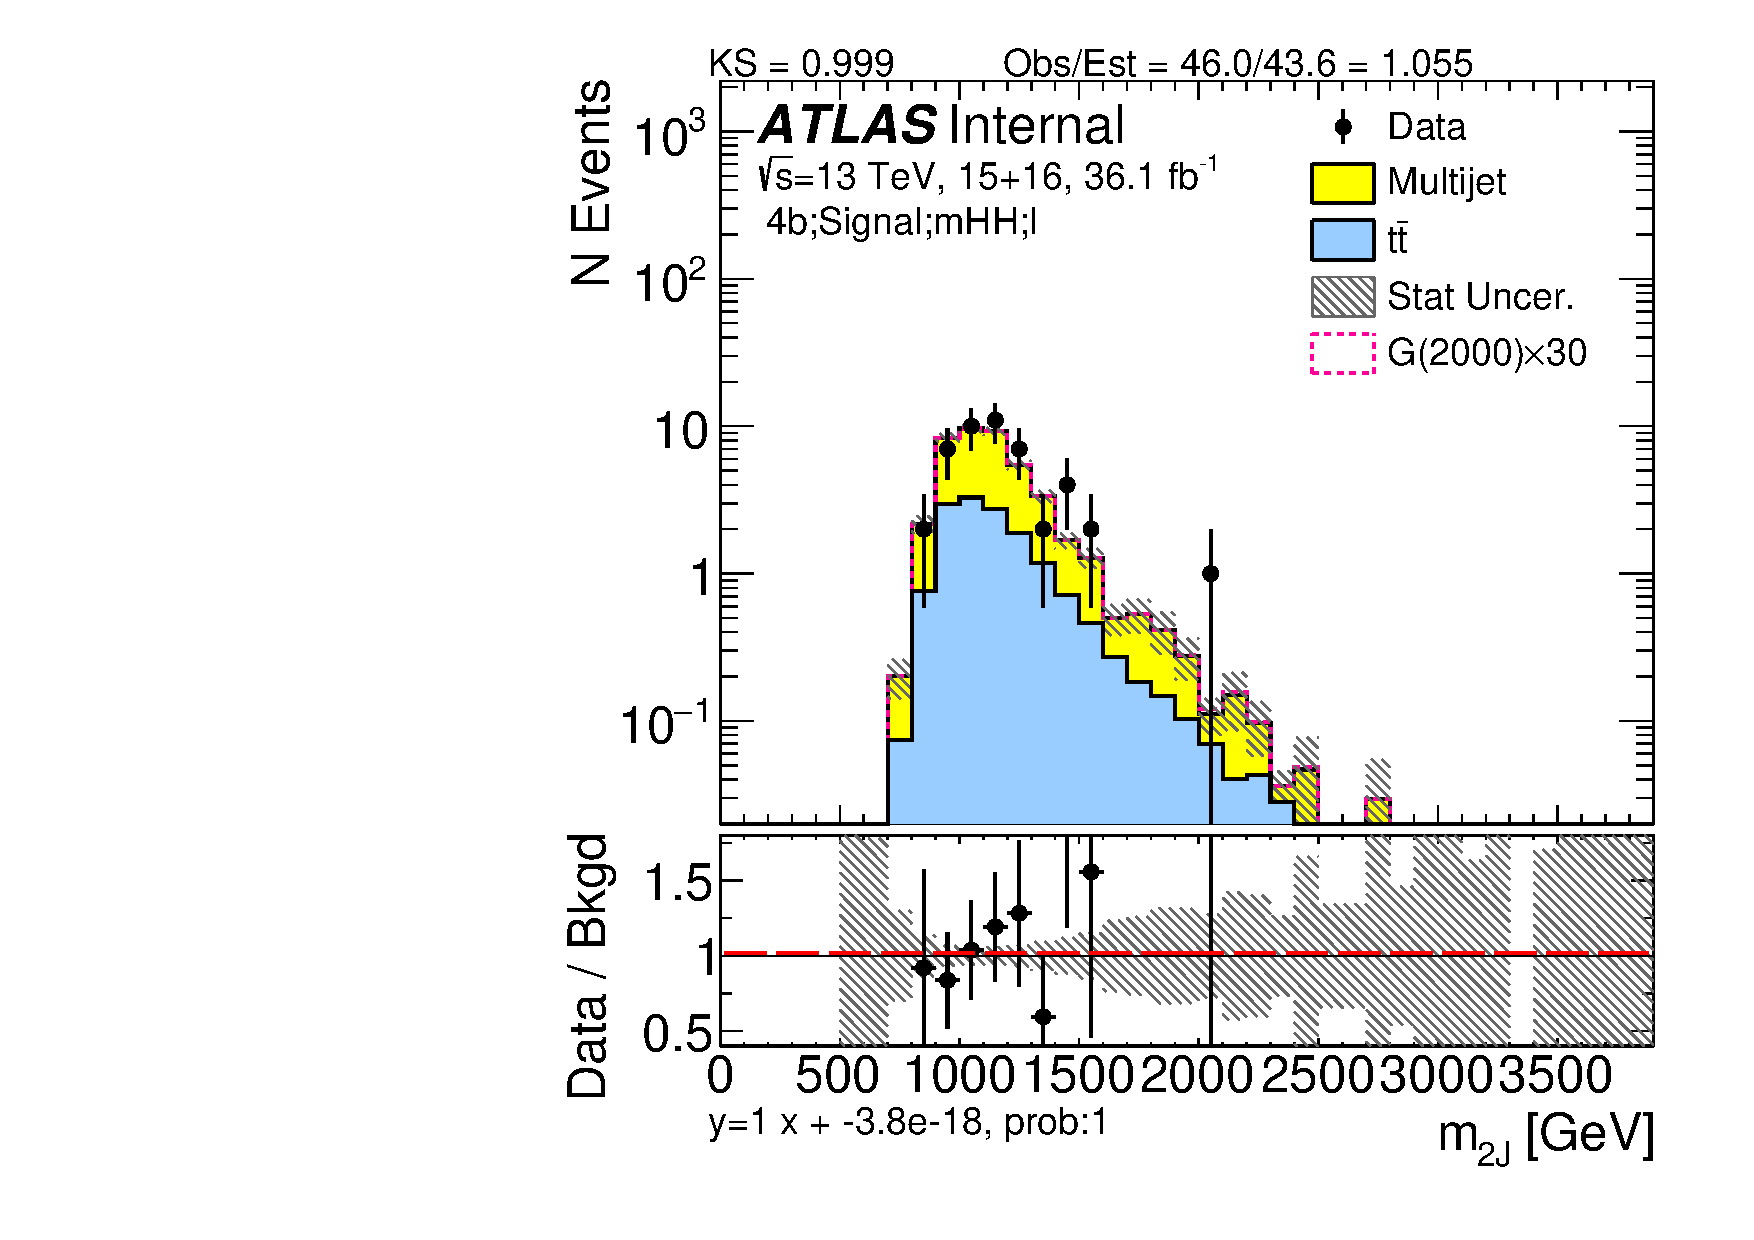
\includegraphics[width=0.45\textwidth,angle=-90]{figures/boosted/TT/Moriond_TT_FourTag_Signal_mHH_l_1.pdf}
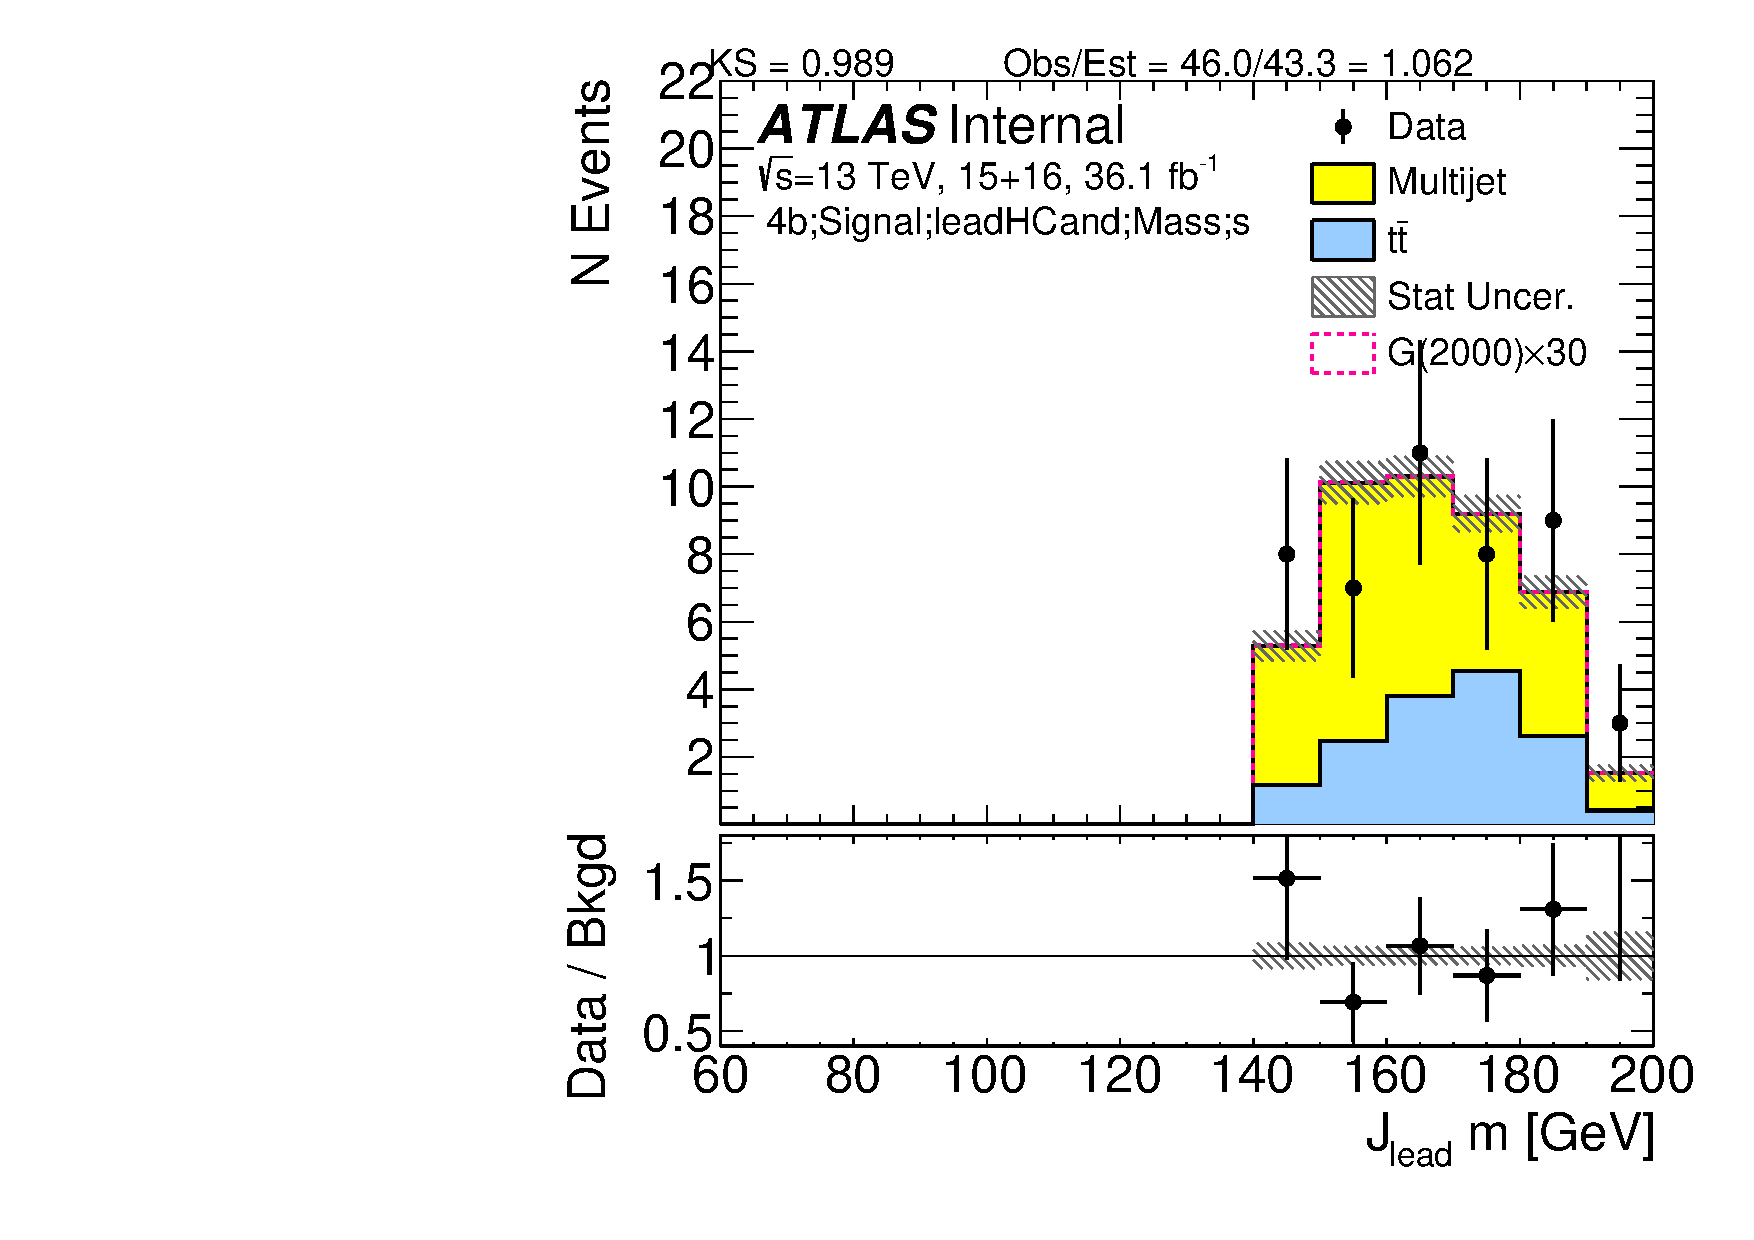
\includegraphics[width=0.45\textwidth,angle=-90]{figures/boosted/TT/Moriond_TT_FourTag_Signal_leadHCand_Mass_s.pdf}\\
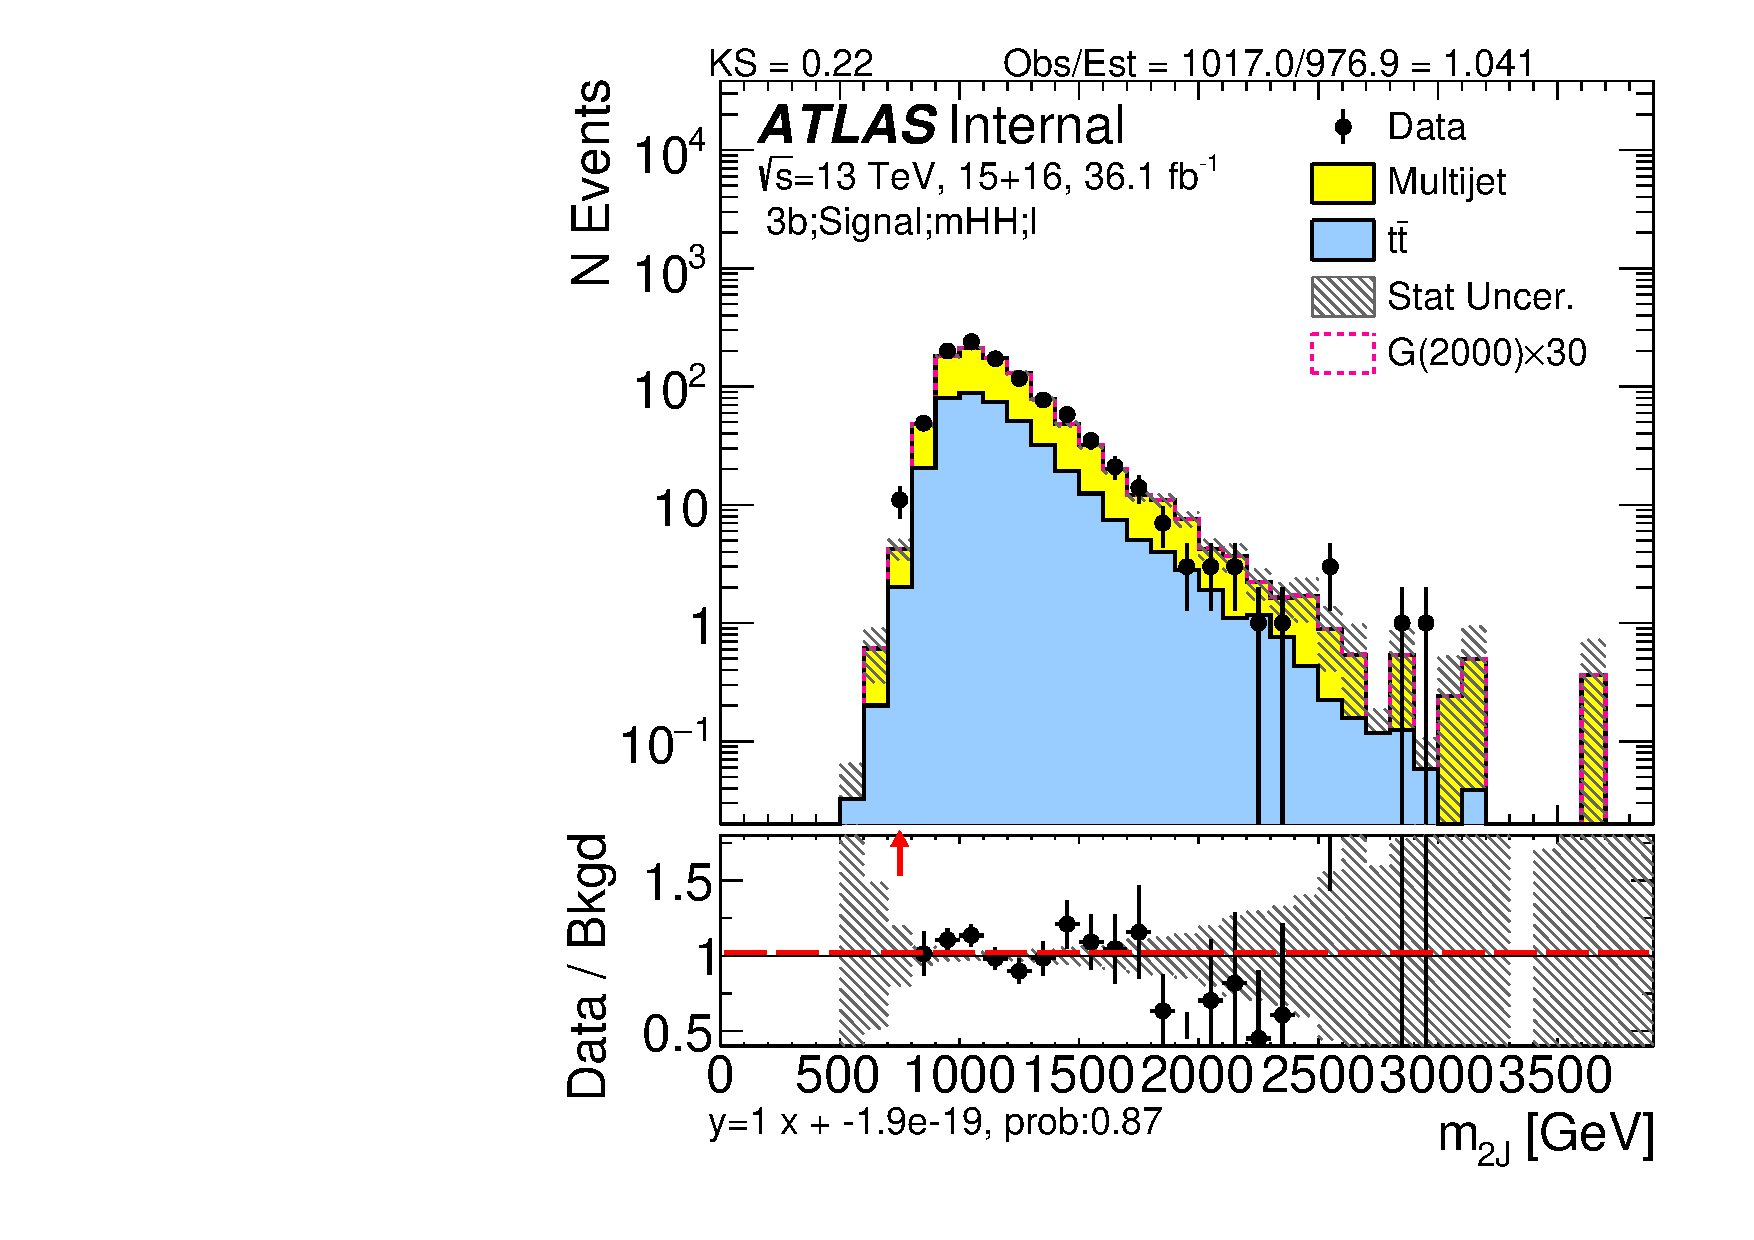
\includegraphics[width=0.45\textwidth,angle=-90]{figures/boosted/TT/Moriond_TT_ThreeTag_Signal_mHH_l_1.pdf}
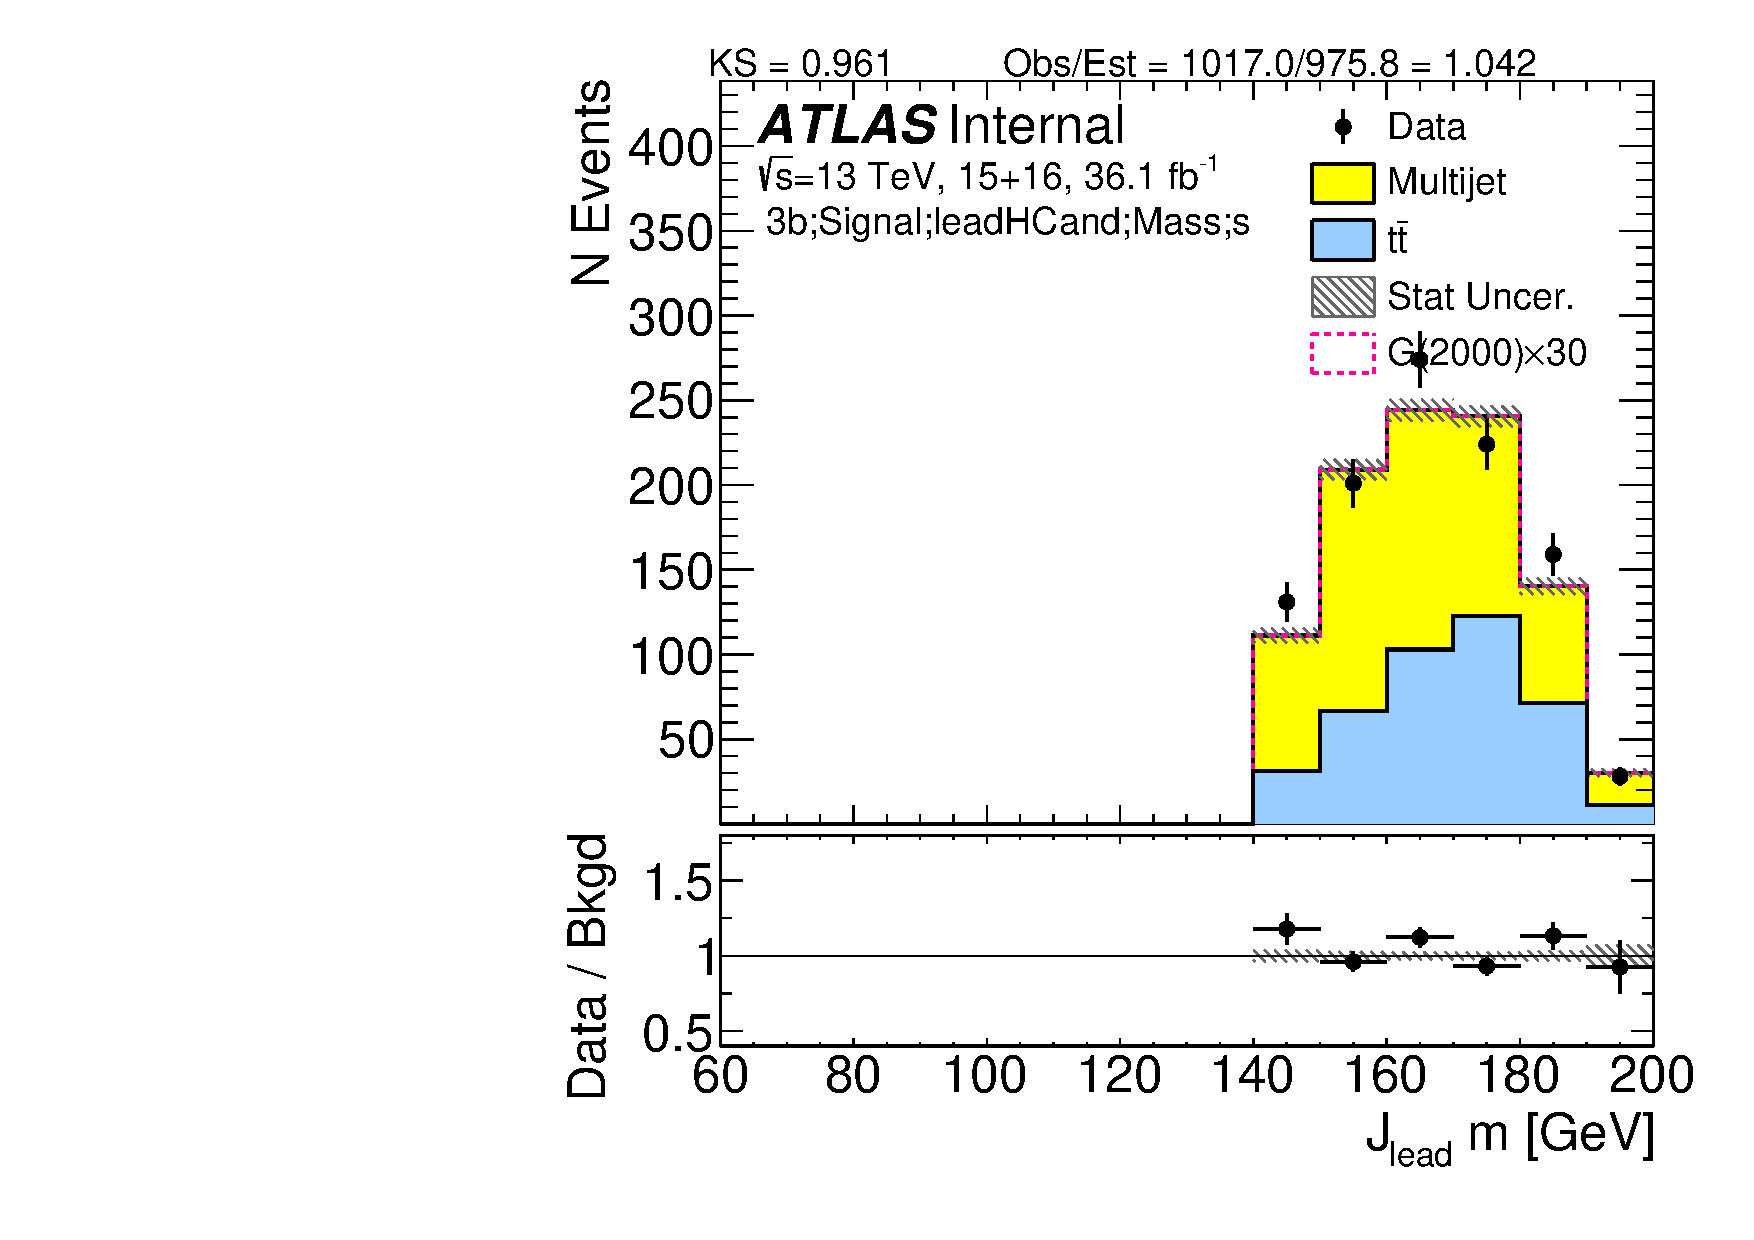
\includegraphics[width=0.45\textwidth,angle=-90]{figures/boosted/TT/Moriond_TT_ThreeTag_Signal_leadHCand_Mass_s.pdf}\\
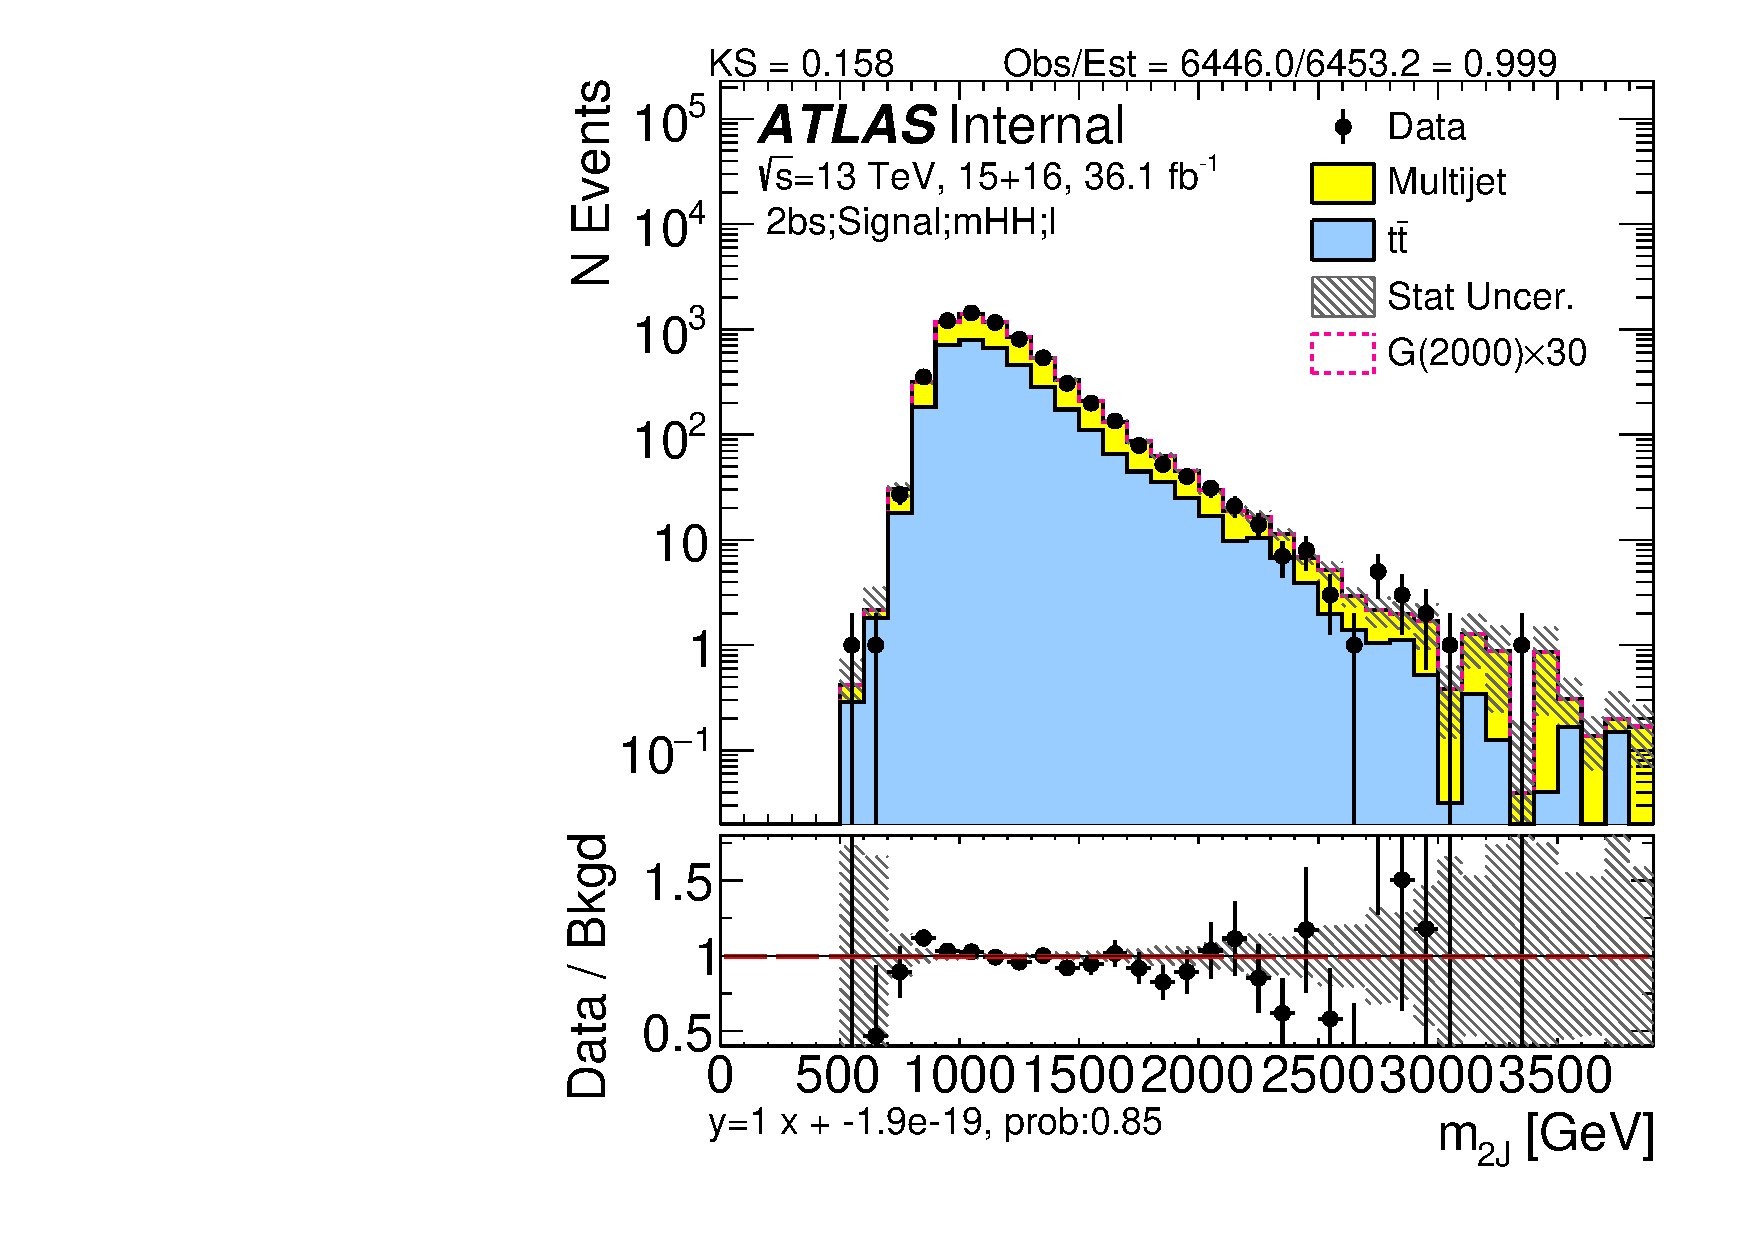
\includegraphics[width=0.45\textwidth,angle=-90]{figures/boosted/TT/Moriond_TT_TwoTag_split_Signal_mHH_l_1.pdf}
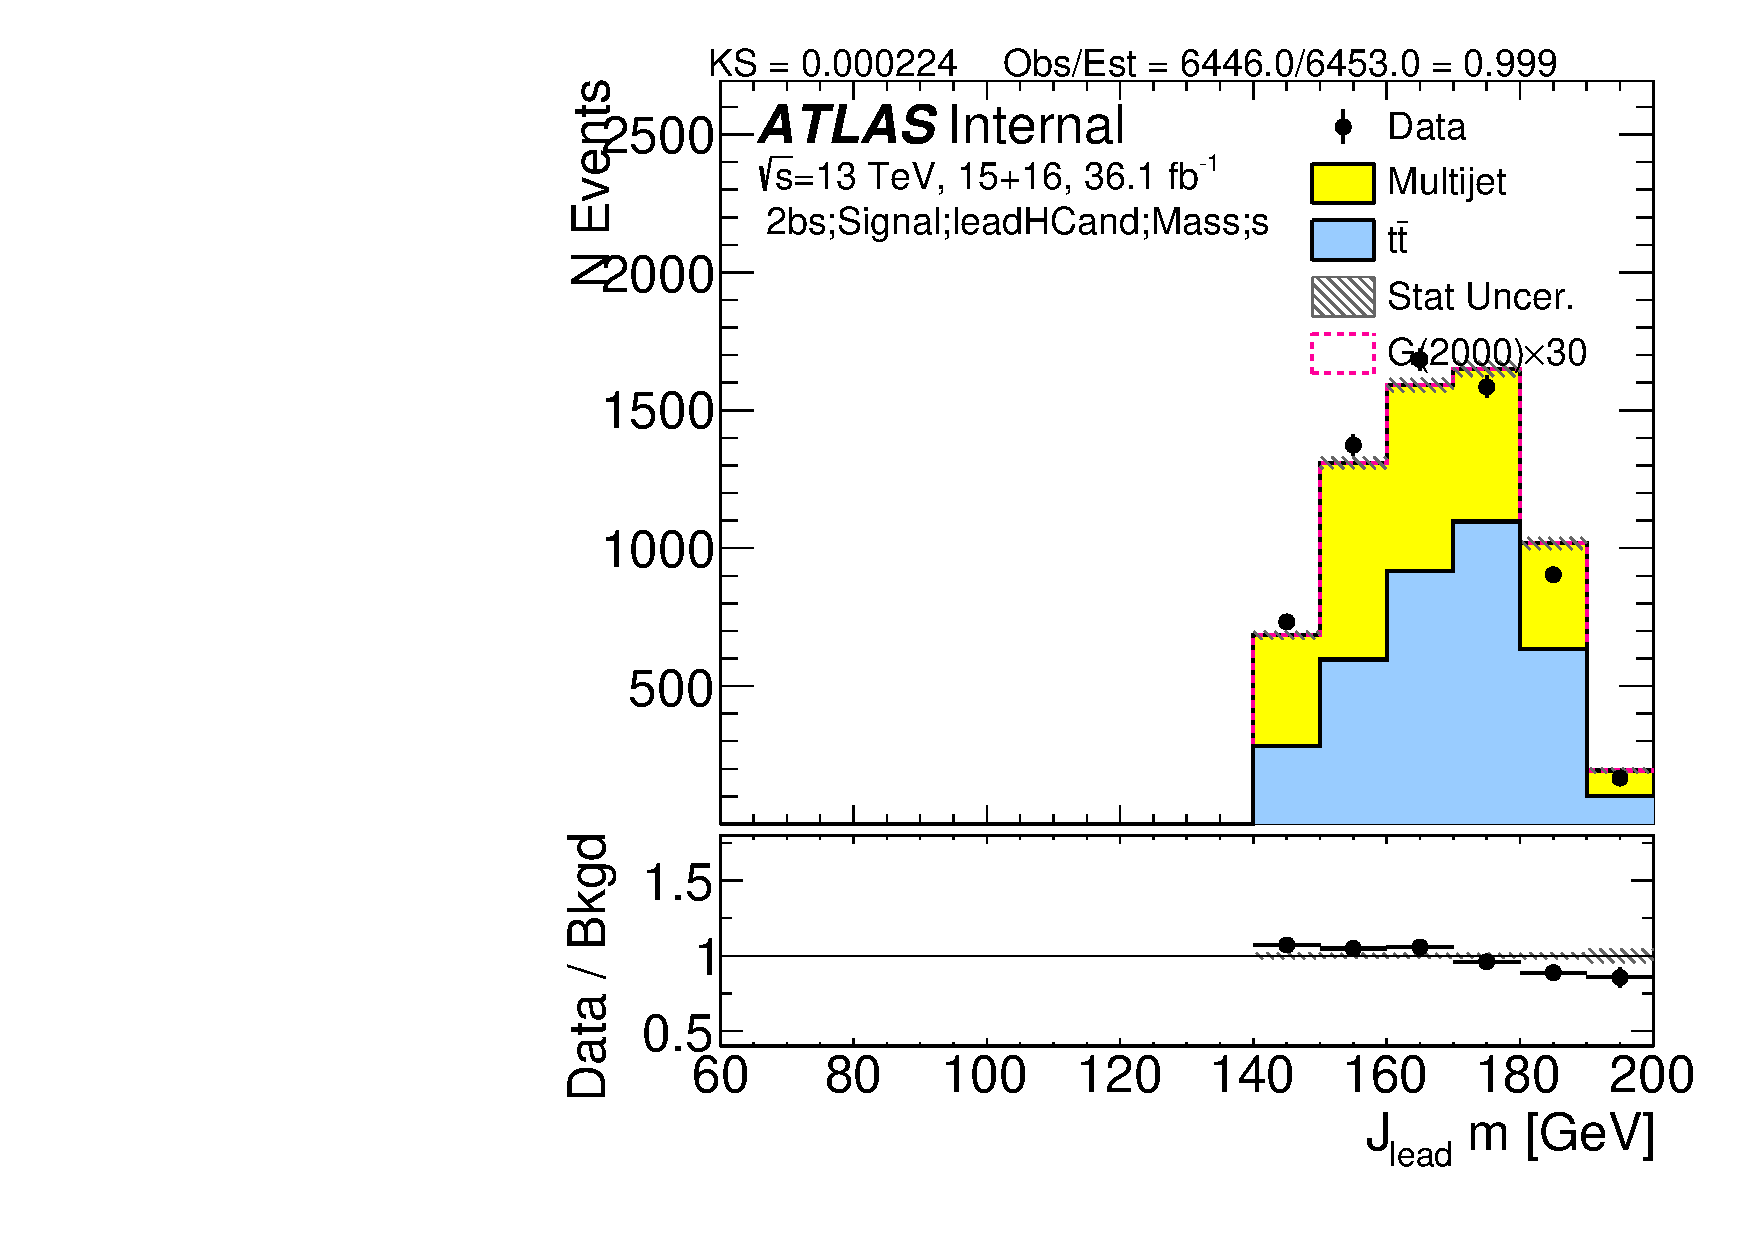
\includegraphics[width=0.45\textwidth,angle=-90]{figures/boosted/TT/Moriond_TT_TwoTag_split_Signal_leadHCand_Mass_s.pdf}\\
\end{center}
\caption{TT signal region distribution of di-jet mass (left column) and leading large-R jet mass (right column) in low mass signal, for $4b$ (top row), $3b$(middle row) and $2b$ split (bottom row). The plots are with only statistical uncertainty.}
\label{CRSB:TTSR_Distribution}
\end{figure}


\clearpage
\subsection{Uncertainty on the shape of the \ttbar\ jet mass in the $4/3b$ signal region}
\label{sec:unc-shape-ttbar-in-sr}

\paragraph{}
Because the 4/$3b$ \ttbar\ MJJ distribution is extremely statistically limited, the 4/$3b$ shape is used to predict the final \ttbar\ background shape in the $2bs$ signal region. In order to estimate the possible shape uncertainty, the $2bs$ and $3b$ sideband shapes are compared in Figure~\ref{fig:ttbar-shapes-signal} (after being normalized to the same area).  The $2bs$ is used as there are not sufficient $4b$ statistics to asses the comparison quality. In order to avoid large statistical uncertainties, the distributions of the $3b$ and $2b$ are smoothed. The ratio of the two smoothed distributions is taken as the shape systematic. We then use this function to apply a bin-by-bin scaling of the \ttbar\ background prediction in the signal region, maintaining the same normalization given by nominal $t\bar{t}$ normalization prediction.

\begin{figure}[htbp!]
\begin{center} 
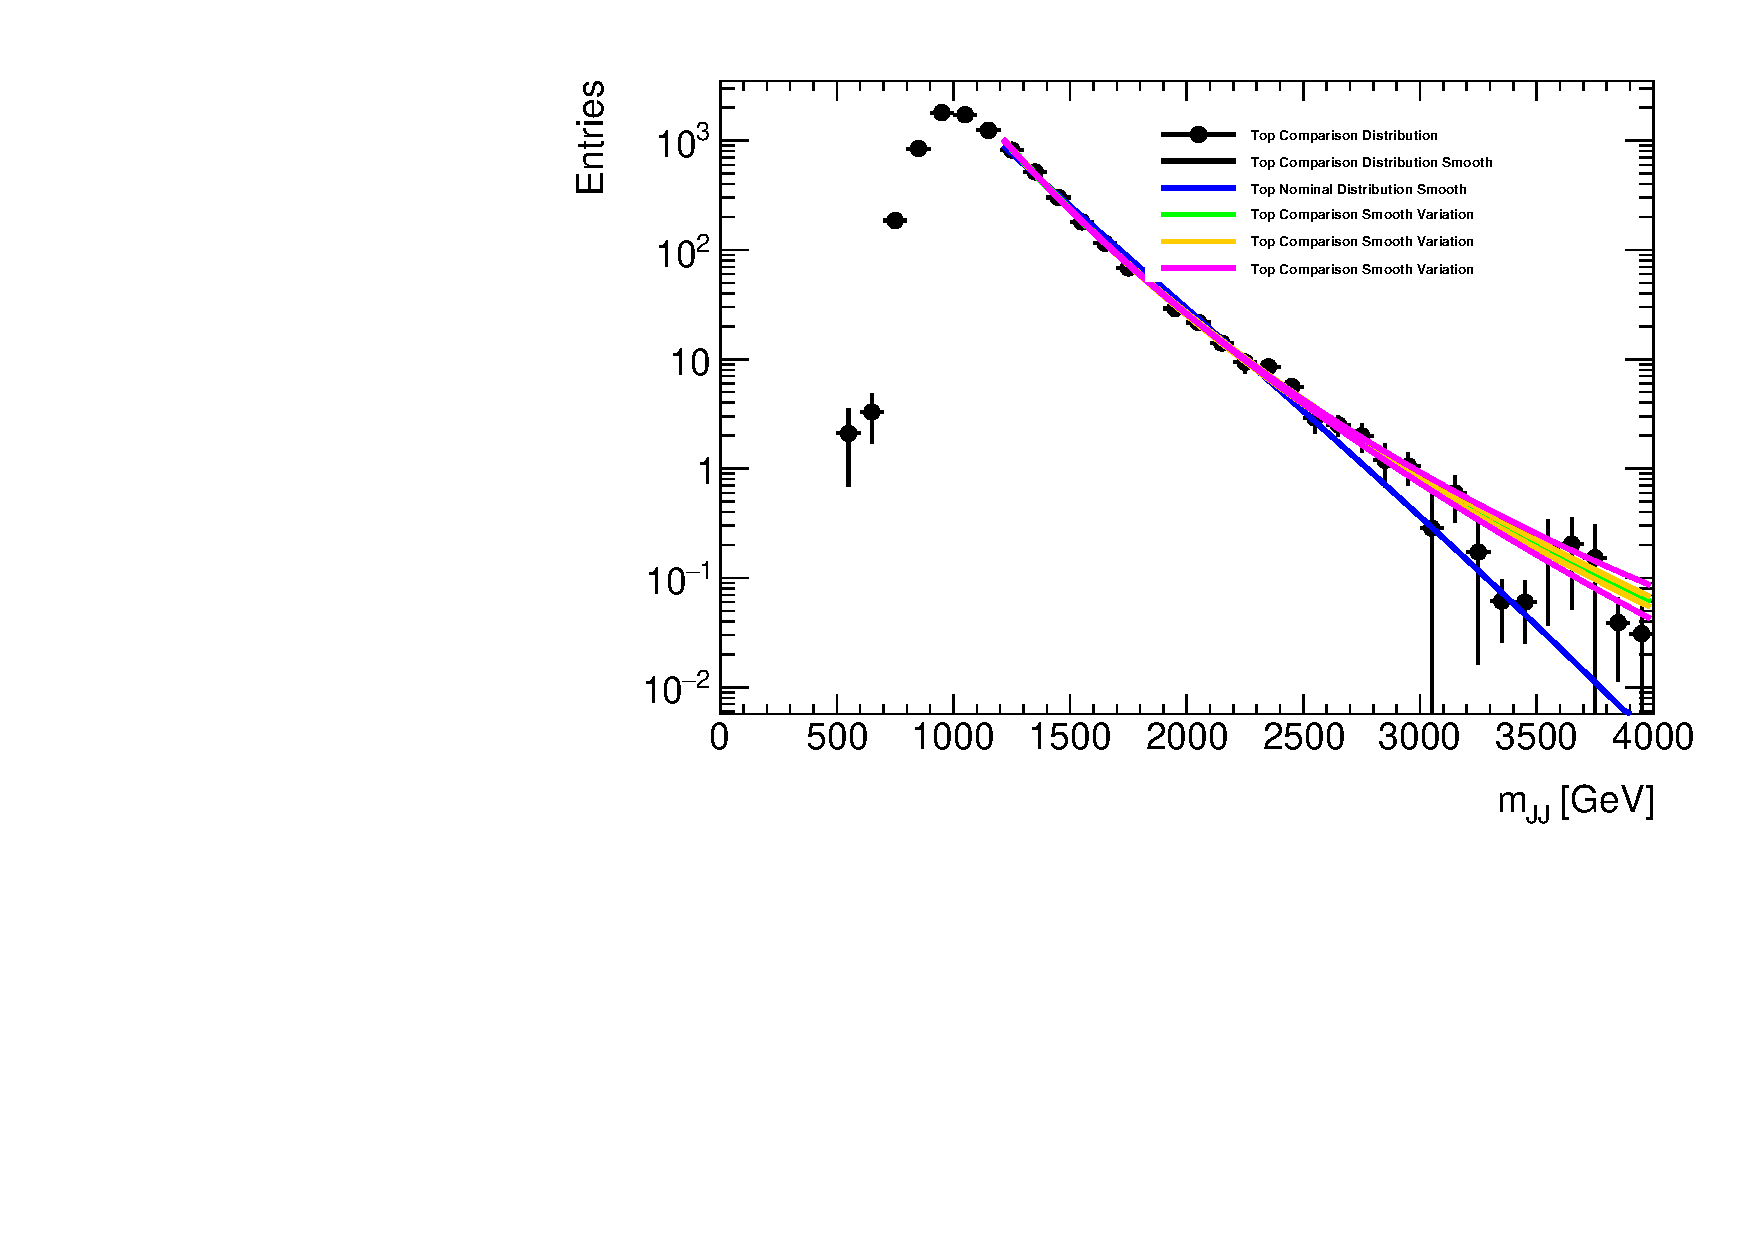
\includegraphics[width=0.31\textwidth,angle=-90]{figures/boosted/Syst_Smooth/TopShapeSRSysfitSmooth_sig33_comp22.pdf}
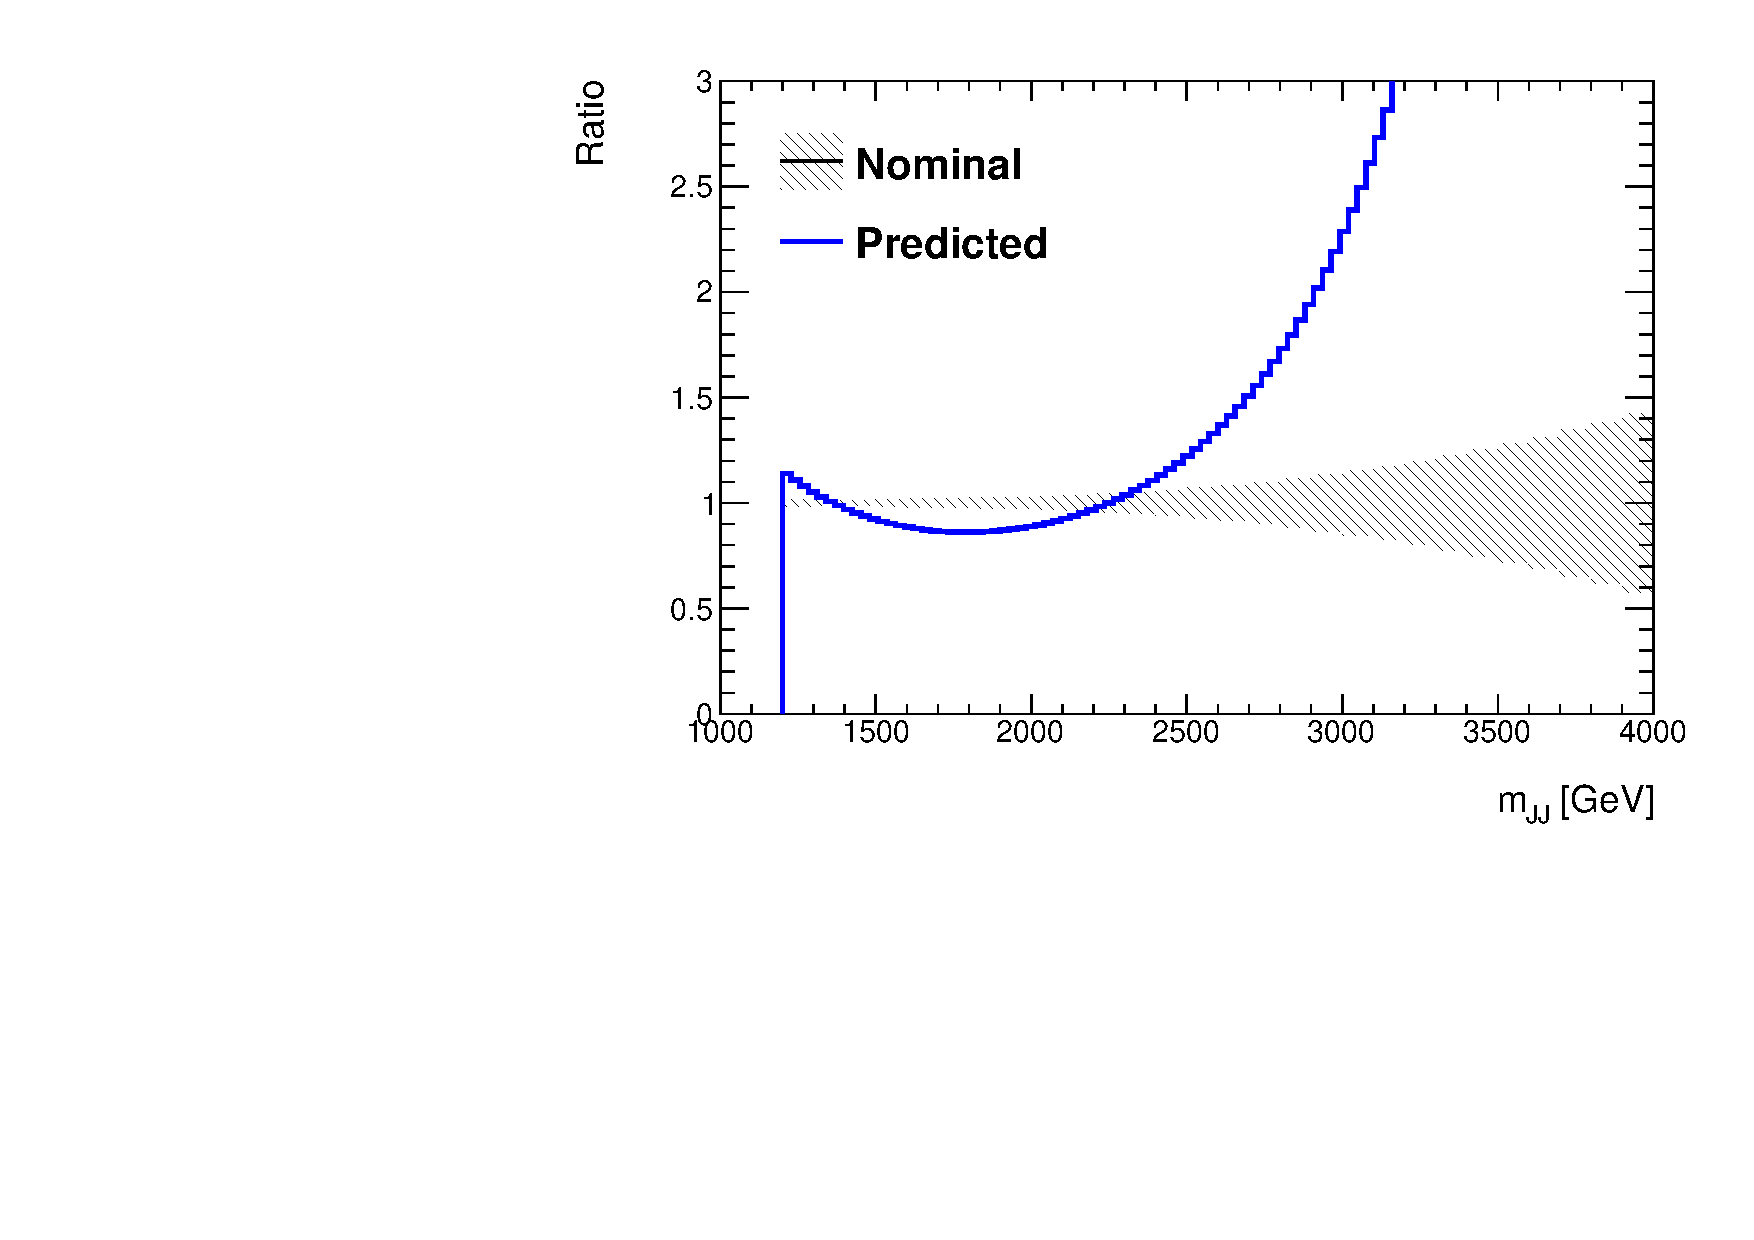
\includegraphics[width=0.31\textwidth,angle=-90]{figures/boosted/Syst_Smooth/TopShapeSRSysfitSmooth_sig33_comp22_ratio.pdf}
\caption{(left)  Shape of the \ttbar\ di-\largeR-jet mass in the sideband region,
comparing the $3b$ shape with that of the $2b$, in order to asses the systematic effect of additional $b$-tags changing the dijet mass distribution.  The $m_{JJ}$ distributions is shown on the left, and the ratio of $3b$ to $2b$ distributions on the right.}
\label{fig:ttbar-shapes-signal}
\end{center}
\end{figure}


\subsection{Uncertainty on the shape of the $1/2b$ QCD distribution in the signal region}
\label{unc-shape-qcd-in-sr}

\paragraph{}
As shown in Figures~\ref{fig:boosted-4b-control-ak10-system} and~\ref{fig:boosted-3b-control-ak10-system}, the shape distribution of the total predicted background using the scaled $1/2b$ QCD sample was found to be in good agreement with the $4b$, $3b$, and $2bs$ data in the control region.  However due to the low statistics in the data in the control region, the comparison is performed by first smoothing the $1/2b$, and the $4/3/2bs$ distributions. The ratio of the smoothed $1/2b$ distributions to that of the smoothed $4/3/2bs$ distributions is taken as the shape systematic. This function is then used to apply a bin-by-bin scaling of the QCD background prediction in the signal region, maintaining the same normalization given by \muqcd.  The CR distributions and the smoothing fit ratios can be found in Figure~\ref{fig:qcd_shape_fit}. This systematics is further split into two parts: one below 2000 \GeV and the other above 2000 \GeV, to ensure the low and high mass shape variation post-fit pulls can vary independently. It should be noted, that this uncertainty is used for both the dijet mass, and the scaled dijet mass distribution, and the correction to to scaling is expected to be small relative to the dijet mass. 

\begin{figure}[htbp!]
\begin{center}
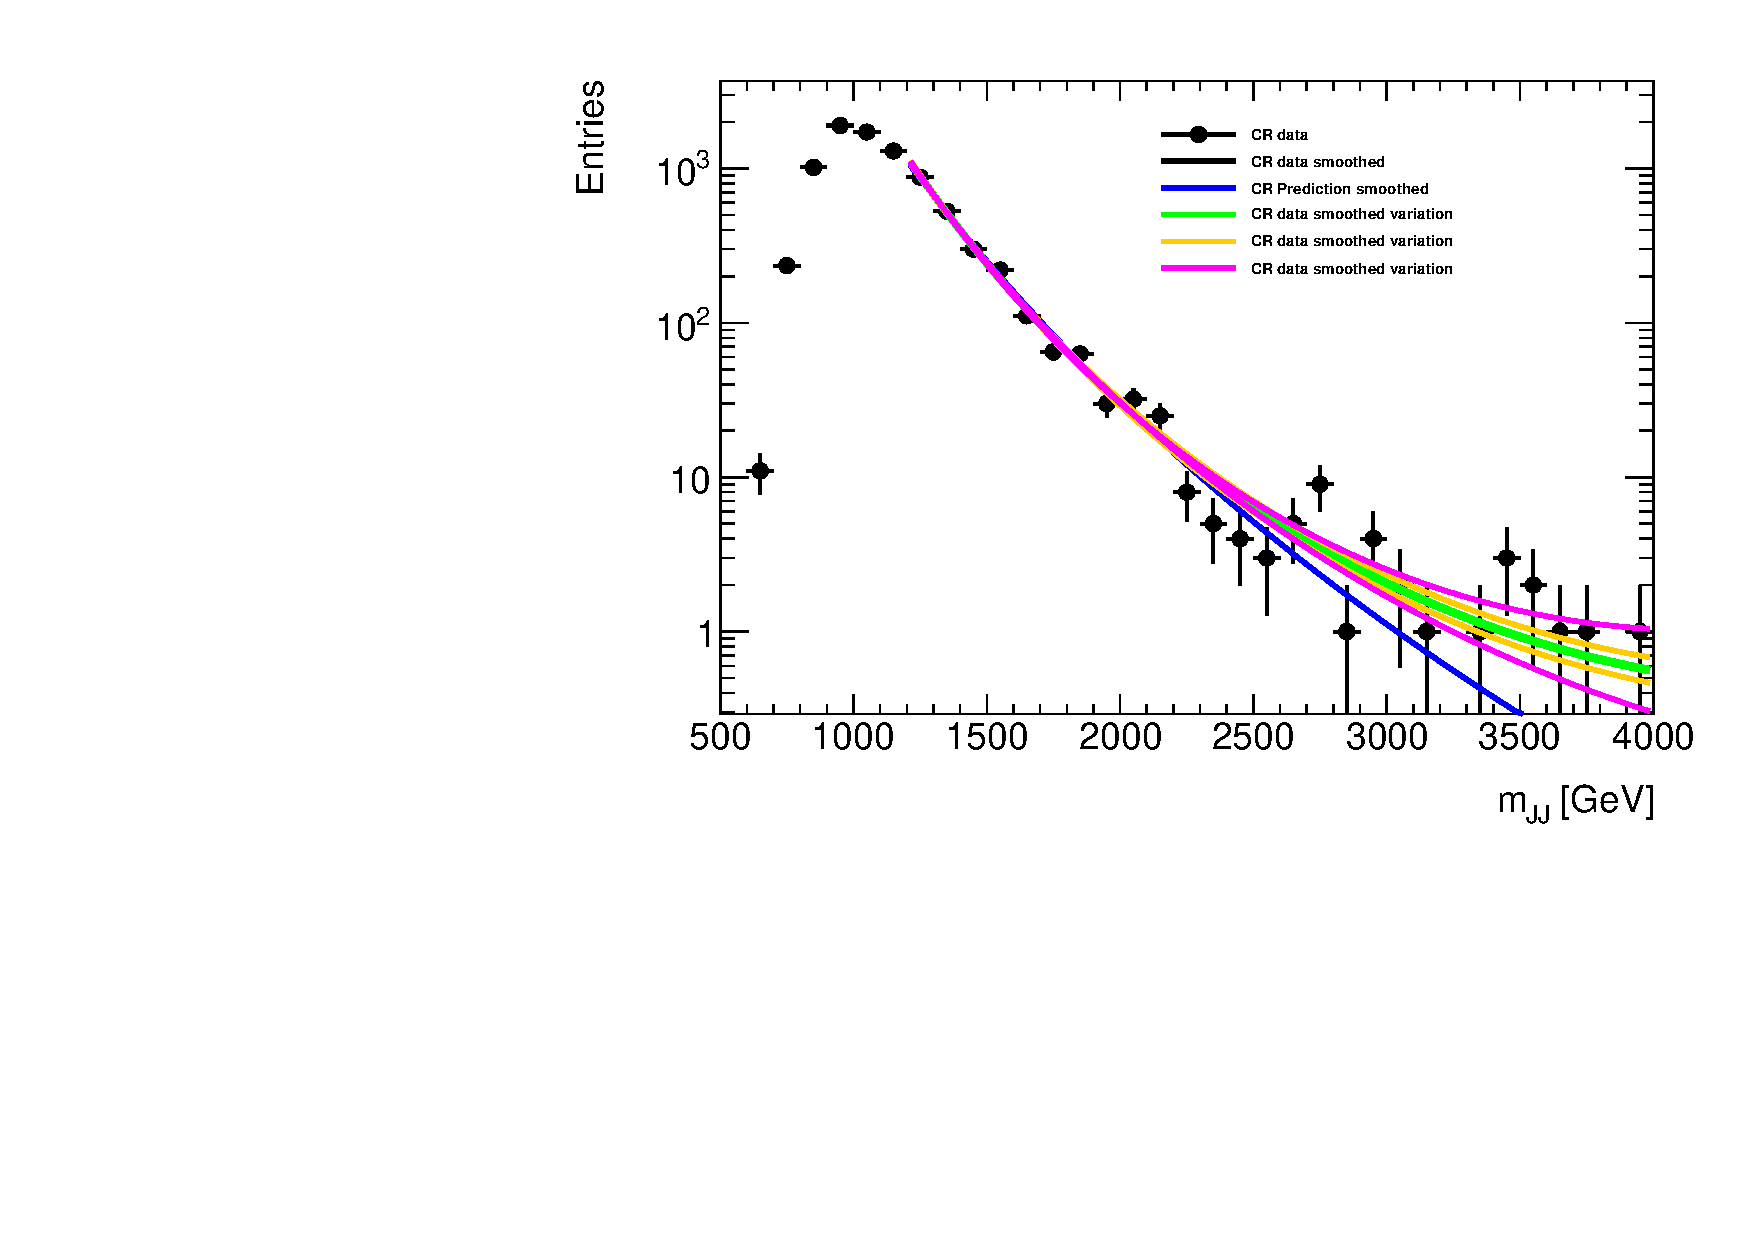
\includegraphics[width=0.31\textwidth,angle=-90]{figures/boosted/Syst_Shape/QCDSysfitSmooth_22.pdf}
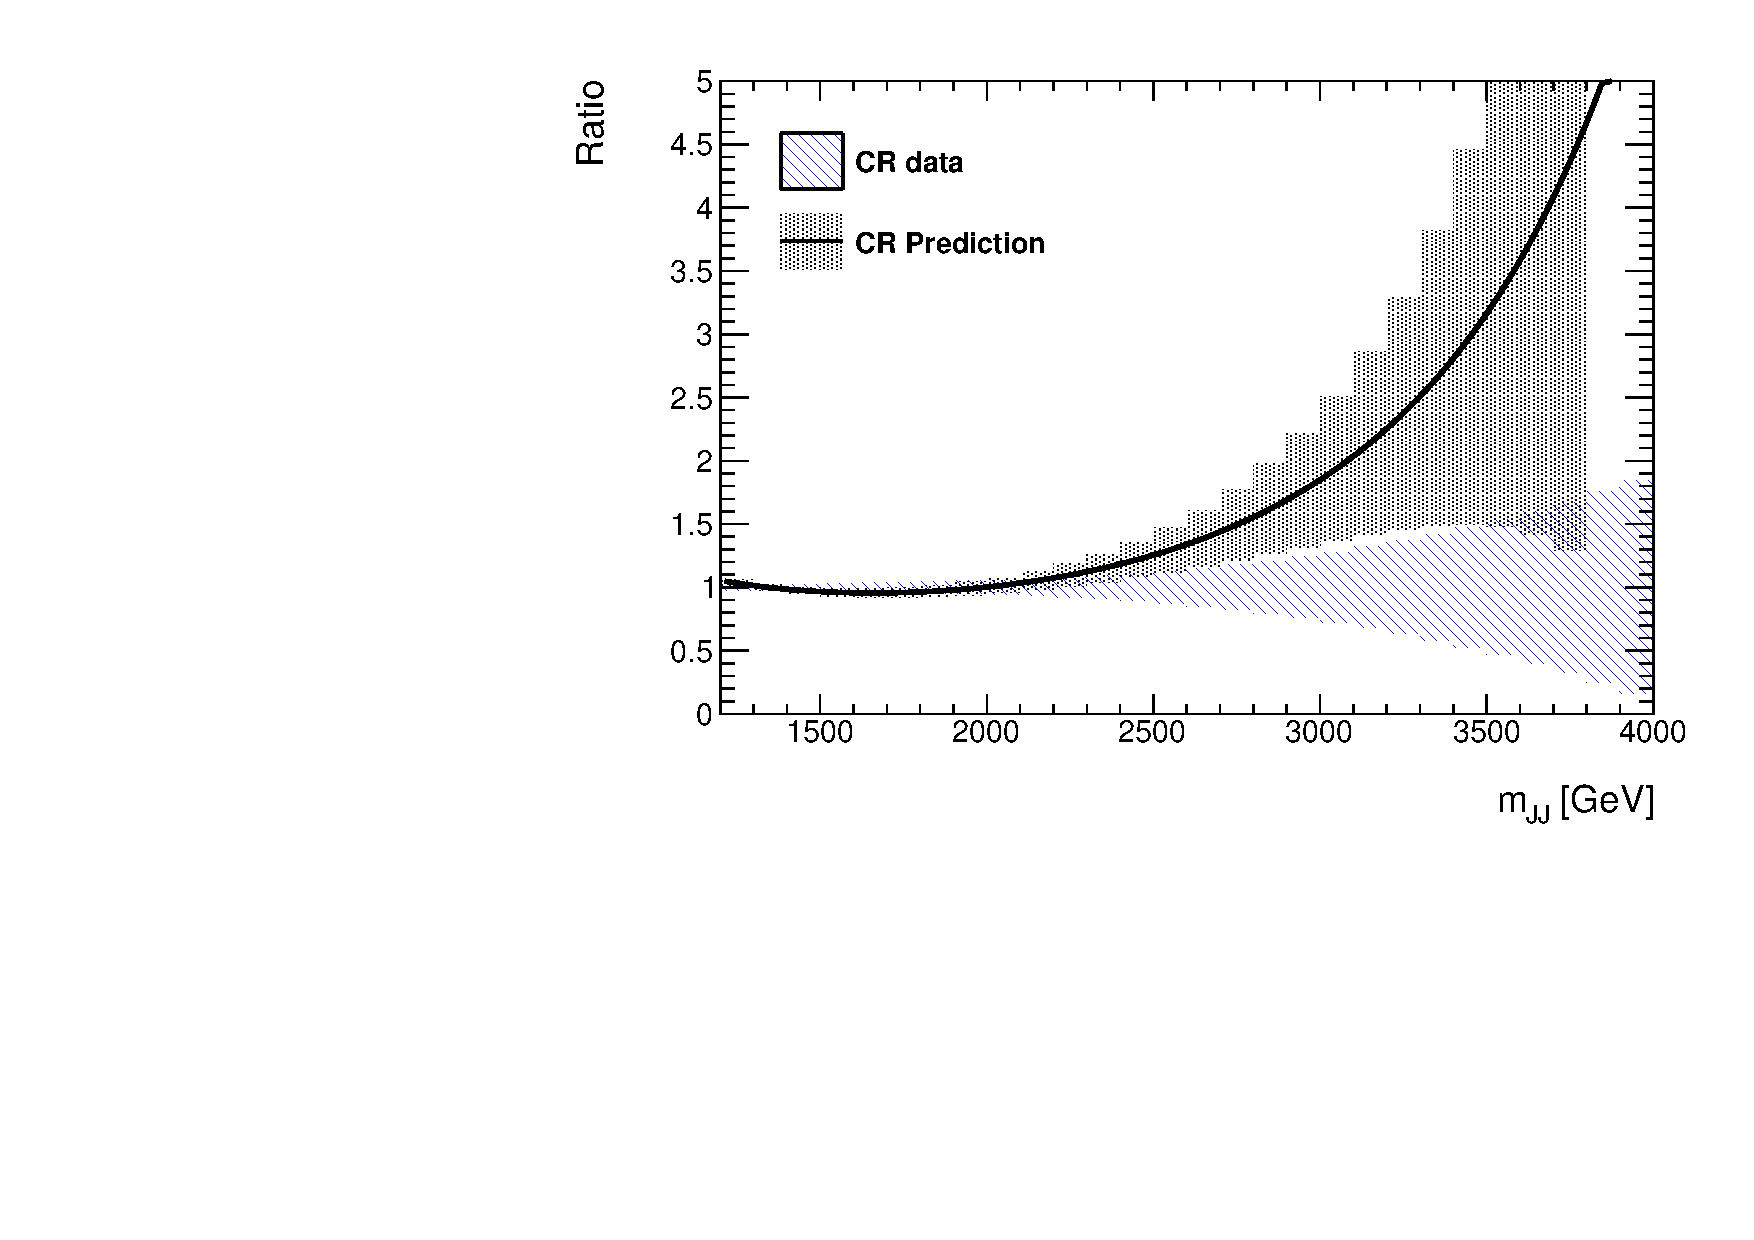
\includegraphics[width=0.31\textwidth,angle=-90]{figures/boosted/Syst_Shape/QCDSysfitSmooth_ratio_22.pdf} \\
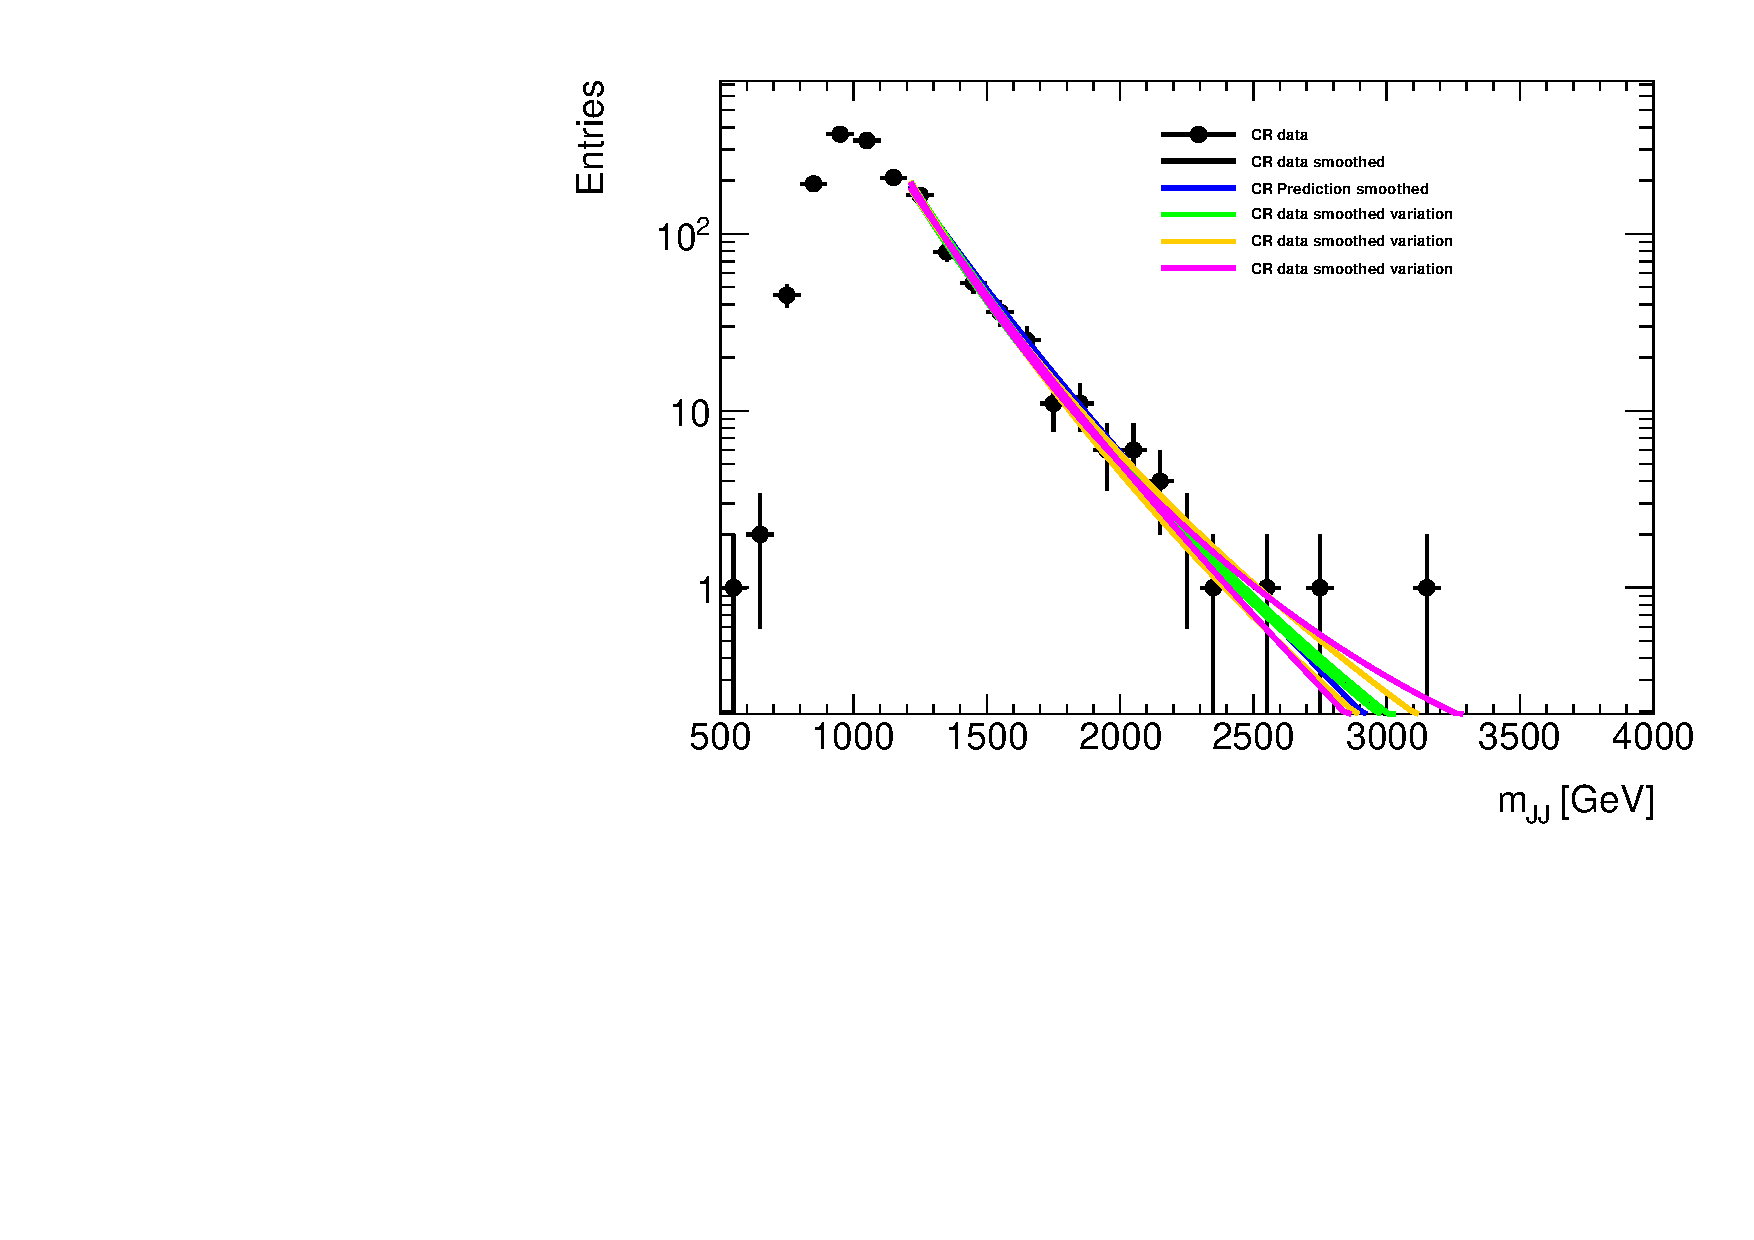
\includegraphics[width=0.31\textwidth,angle=-90]{figures/boosted/Syst_Shape/QCDSysfitSmooth_33.pdf}
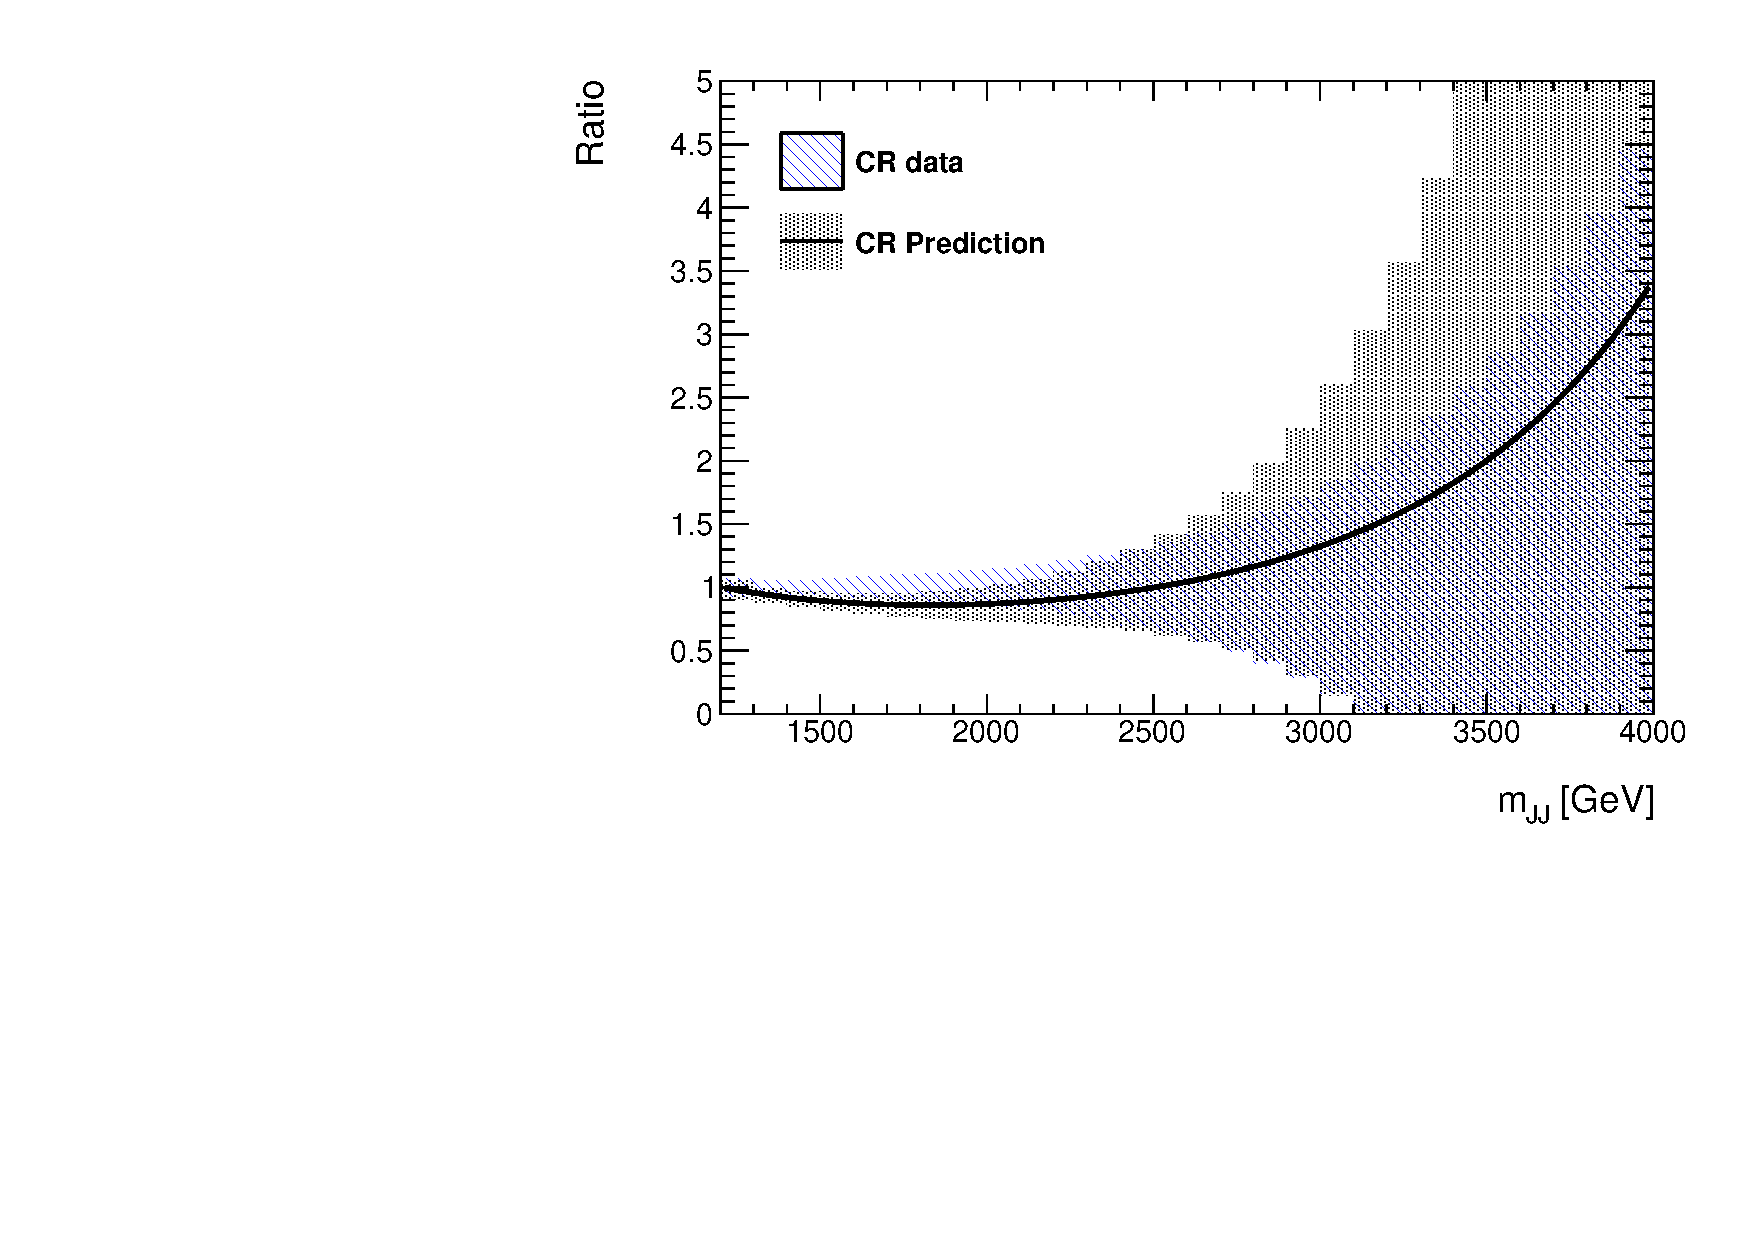
\includegraphics[width=0.31\textwidth,angle=-90]{figures/boosted/Syst_Shape/QCDSysfitSmooth_ratio_33.pdf} \\
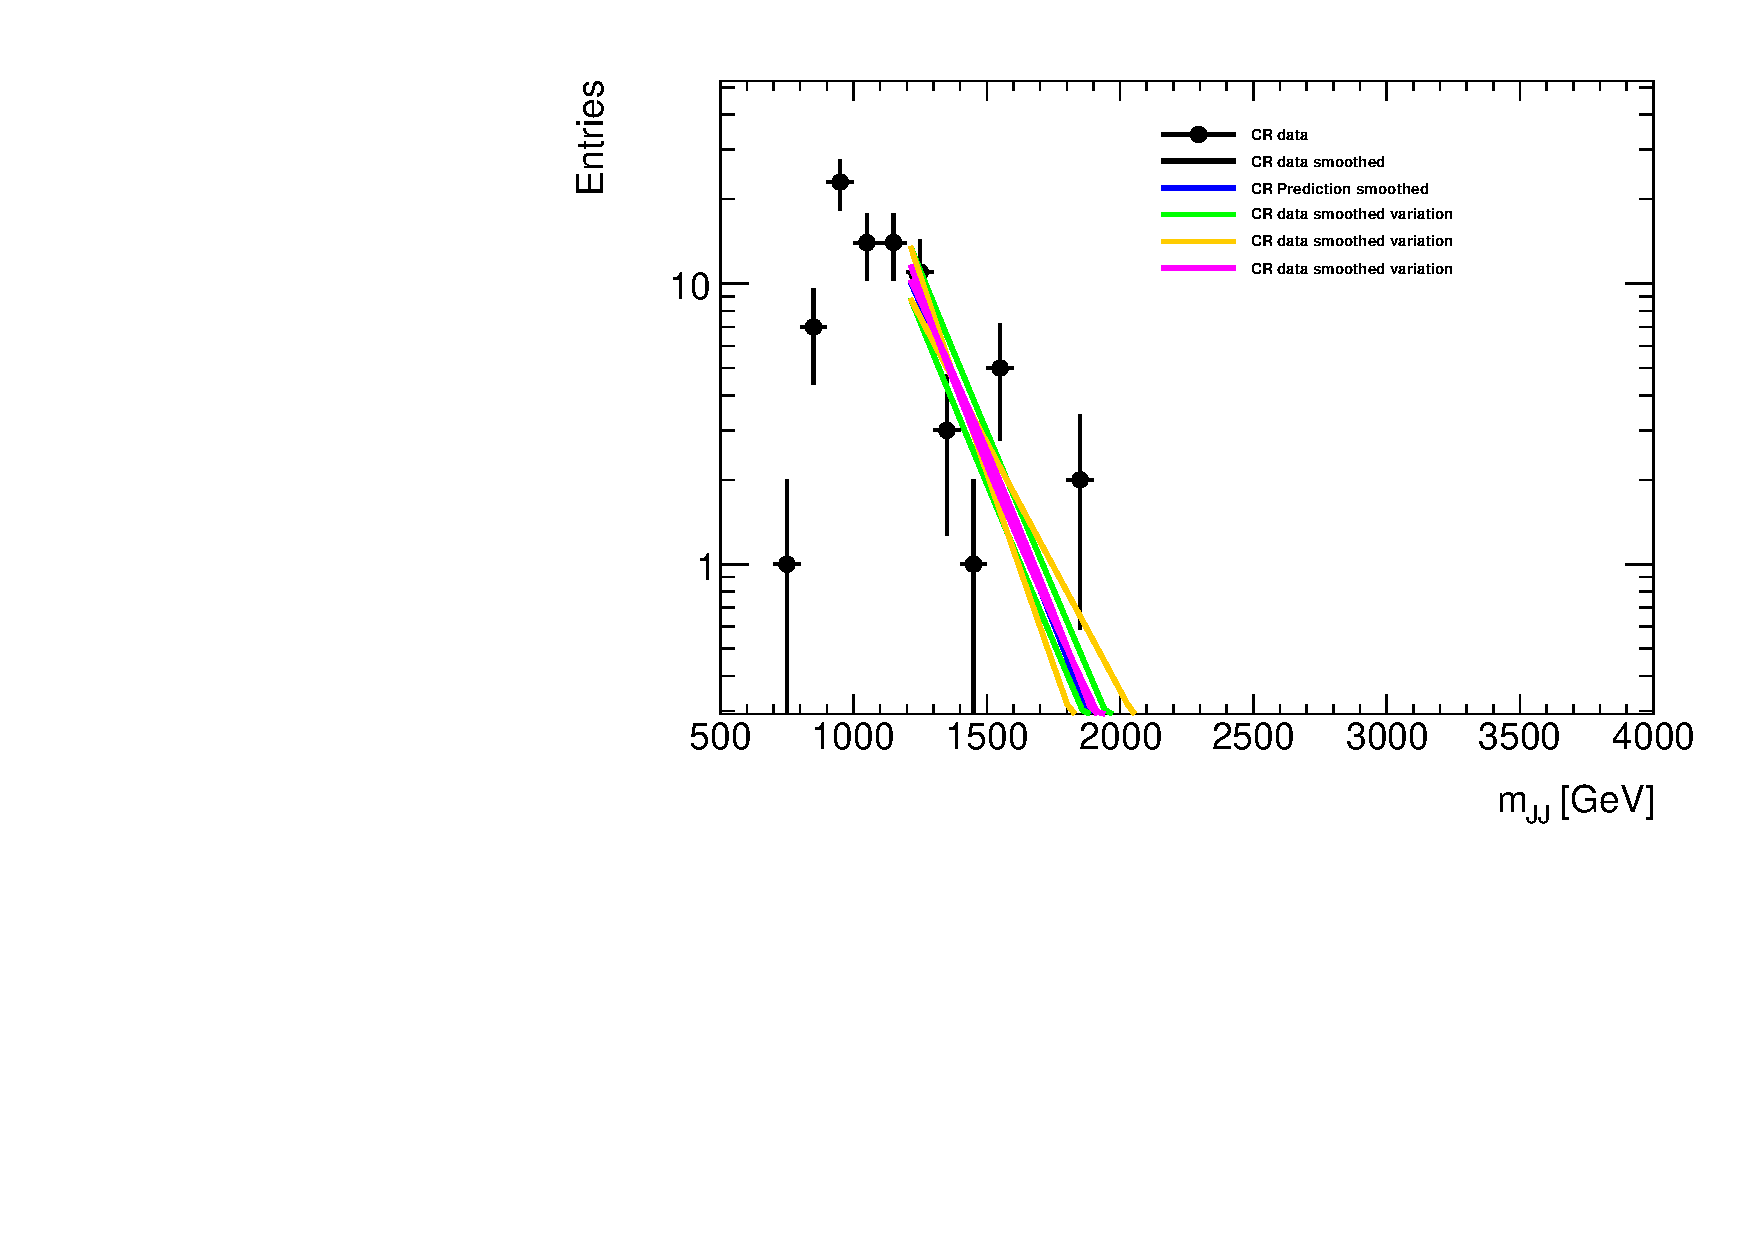
\includegraphics[width=0.31\textwidth,angle=-90]{figures/boosted/Syst_Shape/QCDSysfitSmooth_44.pdf}
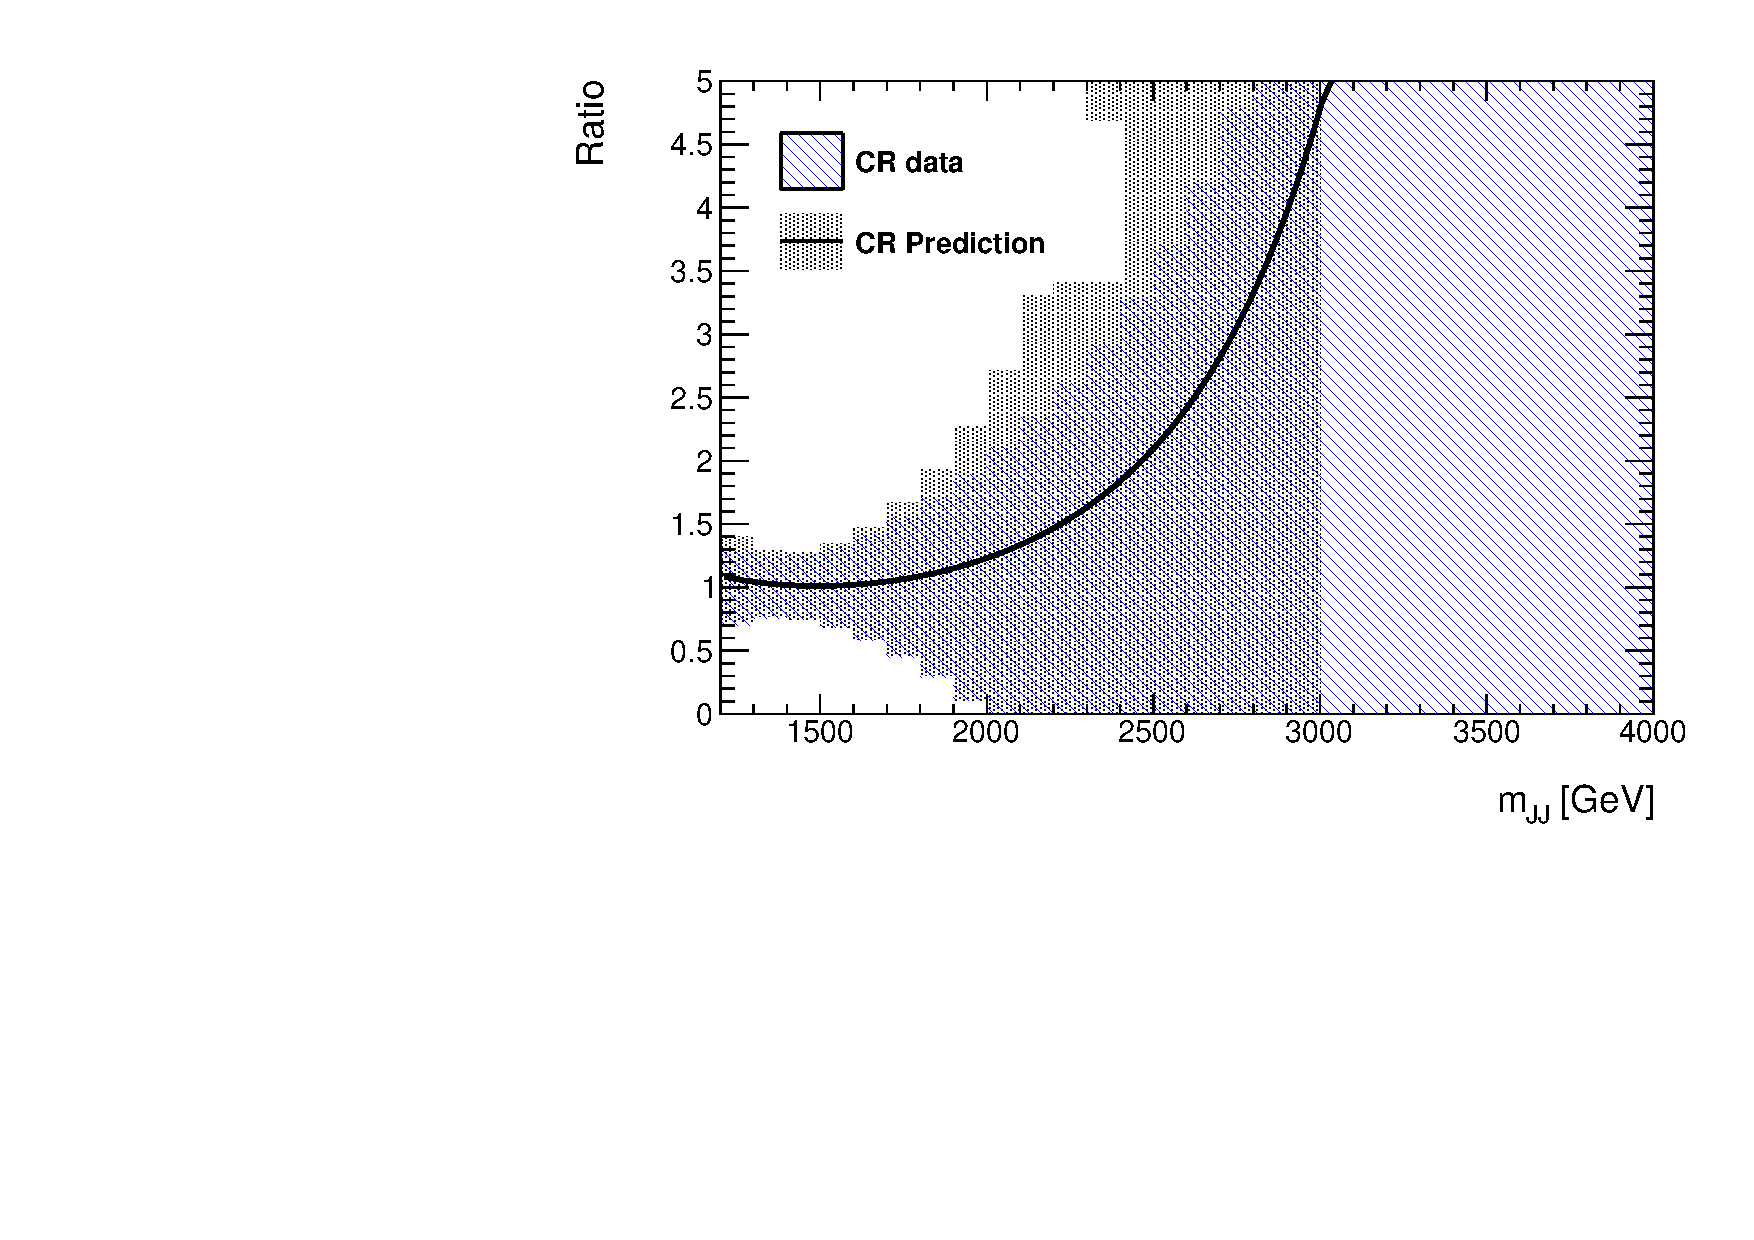
\includegraphics[width=0.31\textwidth,angle=-90]{figures/boosted/Syst_Shape/QCDSysfitSmooth_ratio_44.pdf} \\
\caption{Dijet mass distribution in the CR along with the prediction (left) and the ratio of the prediction to the CR distribution (right)  for the $2bs$ (top) $3b$ (middle) and $4b$ (bottom) samples.  Ratios are from the smoothed distributions, the data uncertainty band contains the smoothing parameter variations, and the prediction uncertainty band also contains smoothing parameter variations.}
\label{fig:qcd_shape_fit}
\end{center}
\end{figure}

\subsection{Uncertainty on QCD smoothing function in the signal region}
\label{unc-smooth-qcd-in-sr}

\paragraph{}
The MJ8 function has been used to fit the QCD background prediction in order to smooth the distribution and provide non-zero background estimates up to dijet masses beyond which we have $1/2b$ statistics.  While this distribution is  observed to fit the $1/2b$ data well, it does not have a concrete physical motivation, and in principle the high mass tail of the distribution could be larger than predicted by an exponential.  Two checks are performed, changing the boundaries where the fit is performed, and changing the fit function.

\paragraph{}
To test the impact of the region in which the fit is performed, we varied the upper bound on the dijet fit region to be each of the values $\{2800,\ 3000,\ 3200\}$ GeV and the starting value between $\{1200,\ 1300,\ 1400\}$ GeV.  The ratio of the fits for each upper bound, to that of the nominal (1200-3000 GeV) can be found in Figure~\ref{fig:qcd_fit_range_sys_ratio-scaled}, along with a hash band showing the statistical uncertainty of the nominal fit.  The maximum deviation from the nominal fit, per bin, is taken as the shape systematic uncertainy.  This is estimated separately for $2bs$, $3b$, and $4b$ samples.

\paragraph{}
It should be noted that fits in which the fit $\chi^2$ probability was less than 0.001\%, or in which the fit integrals between 1500-2000 GeV, 2000-2500 GeV, or $>$2500 GeV were not in agreement with the original $1/2b$ distribution within a factor of 2 or 0.5, were not used to estimate the uncertainty.  The aforementioned checks ensure that we do not use poor fits of the $1/2b$ distribution to estimate the uncertainty.

\begin{figure}[htbp!]
\begin{center}
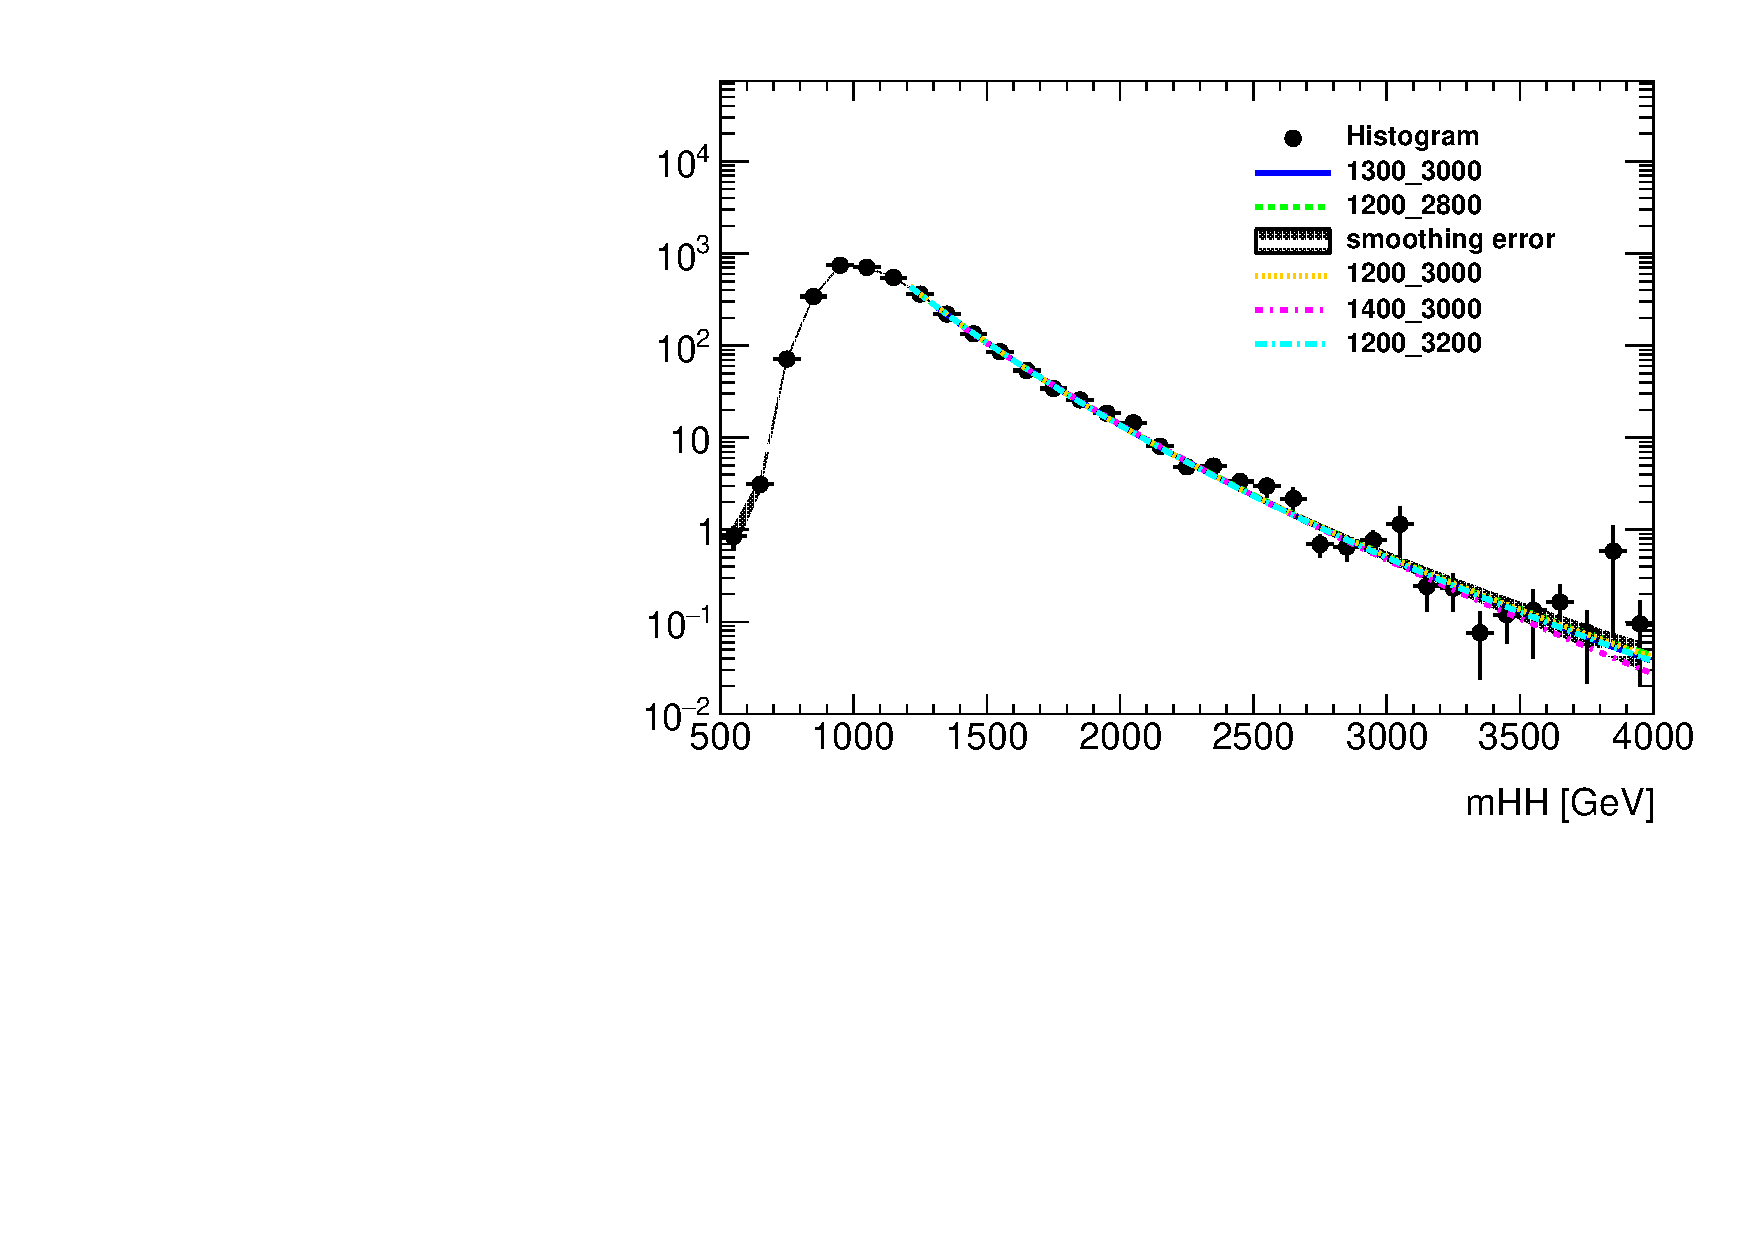
\includegraphics[width=0.31\textwidth,angle=-90]{figures/boosted/Syst_Smooth/smoothFuncRangeCompare_22_comp.pdf}
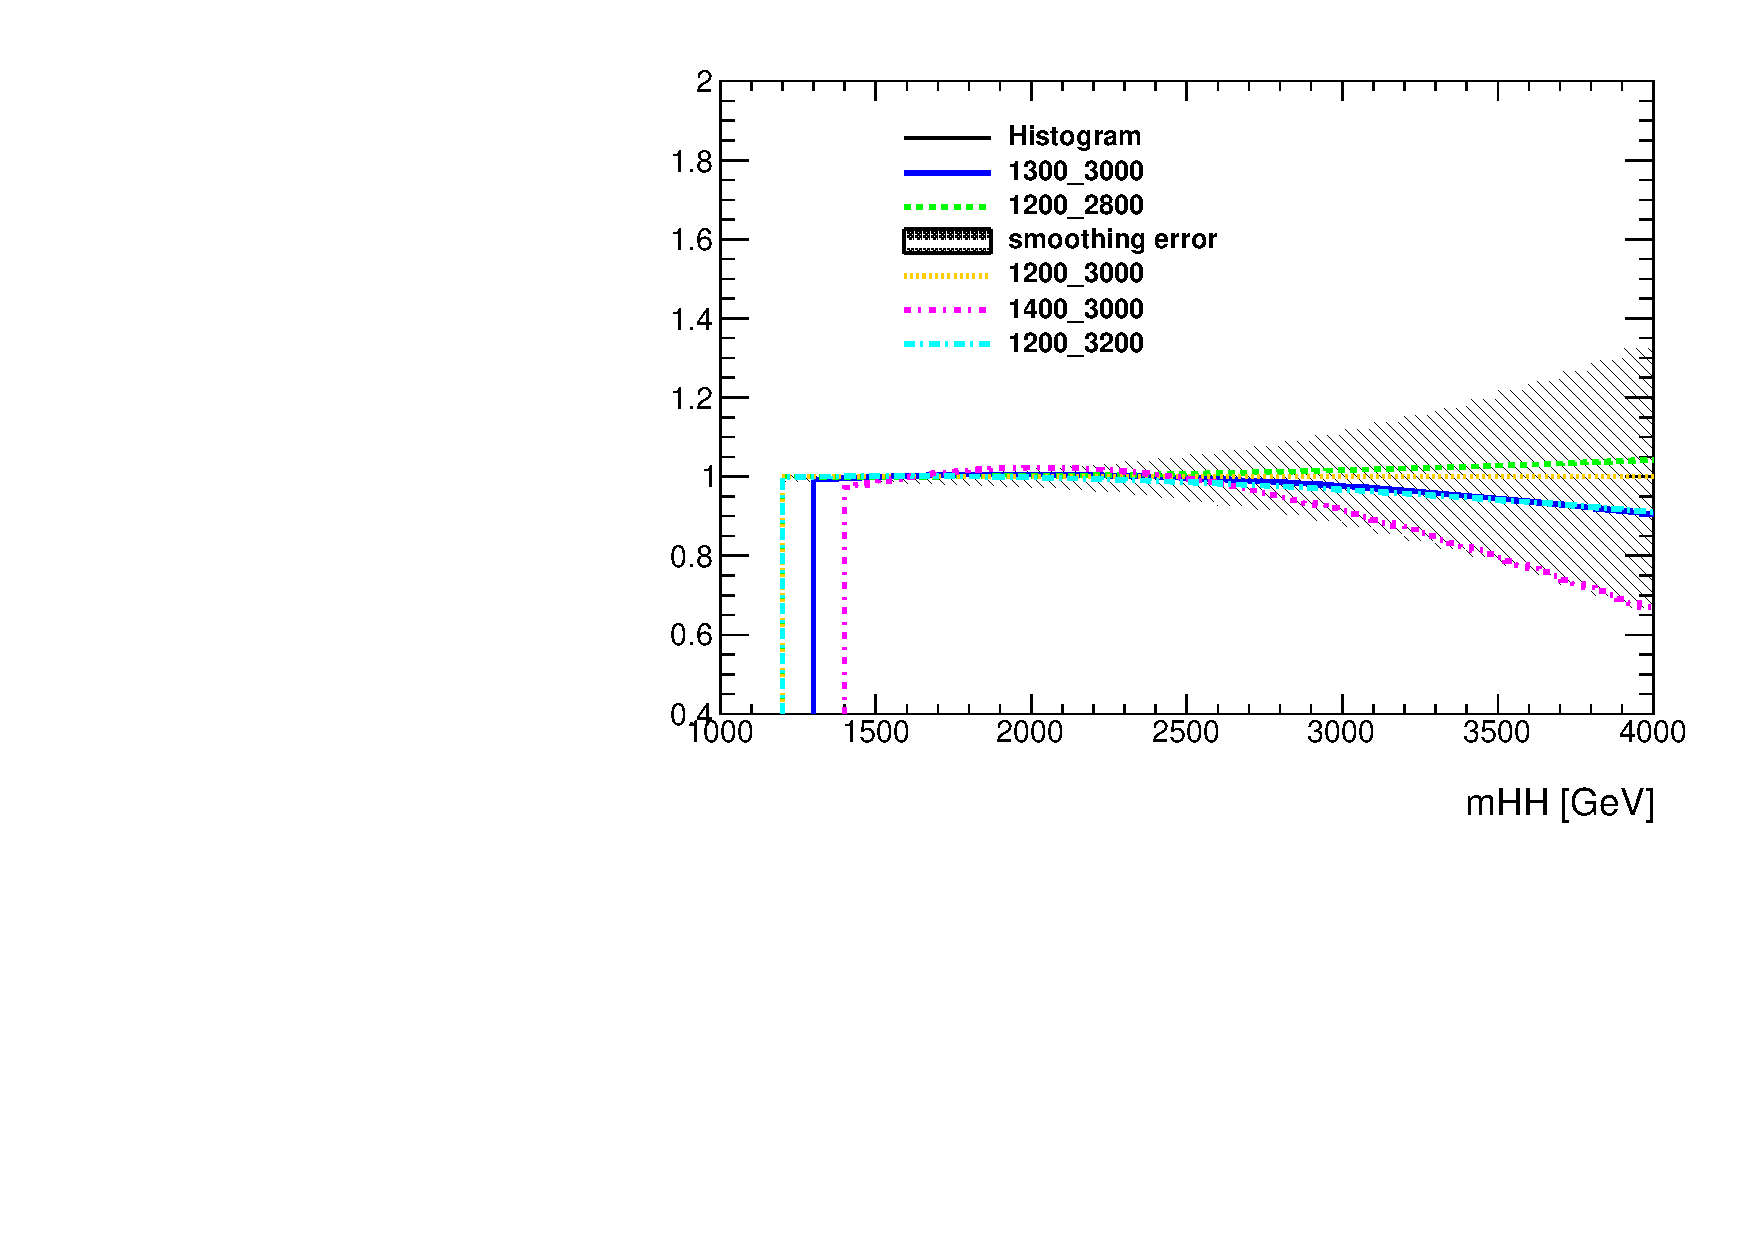
\includegraphics[width=0.31\textwidth,angle=-90]{figures/boosted/Syst_Smooth/smoothFuncRangeCompare_22_comp_ratio.pdf} \\
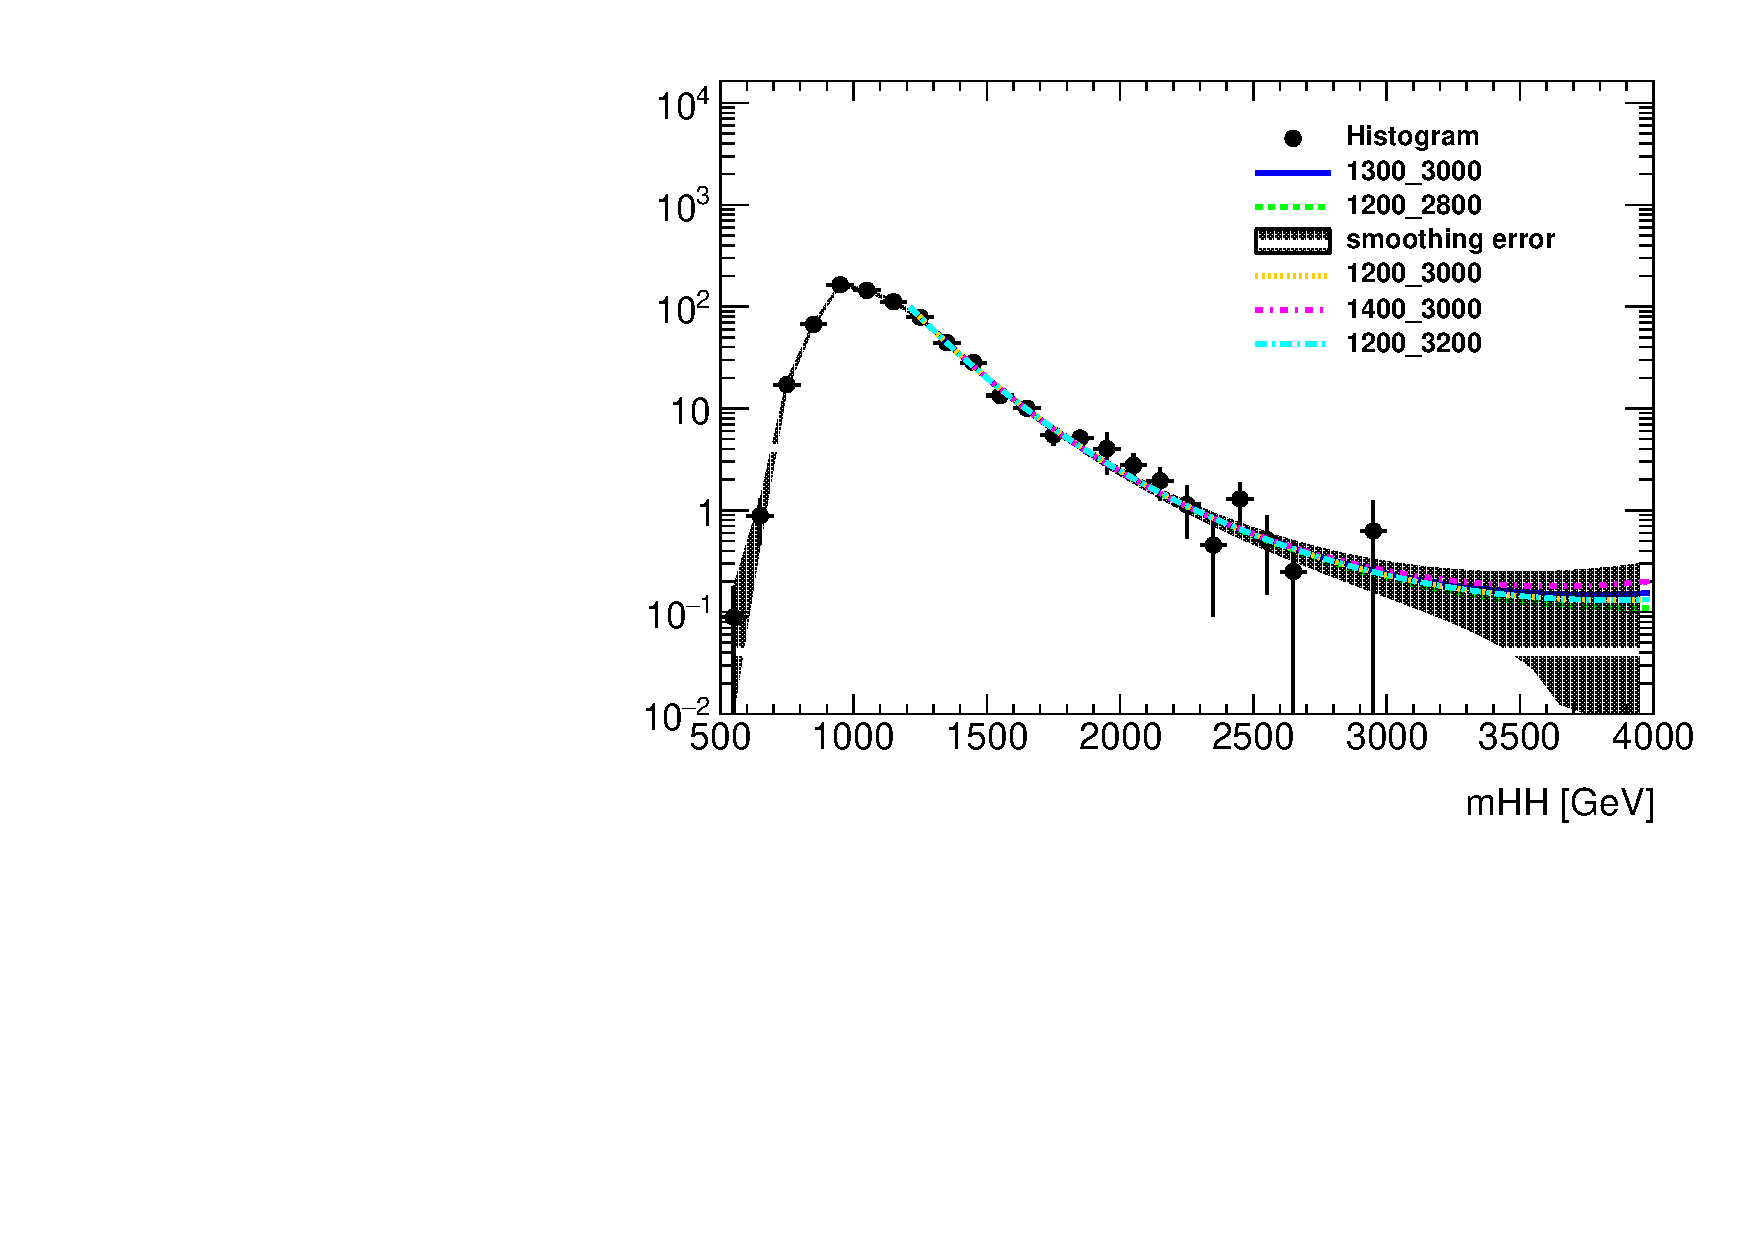
\includegraphics[width=0.31\textwidth,angle=-90]{figures/boosted/Syst_Smooth/smoothFuncRangeCompare_33_comp.pdf}
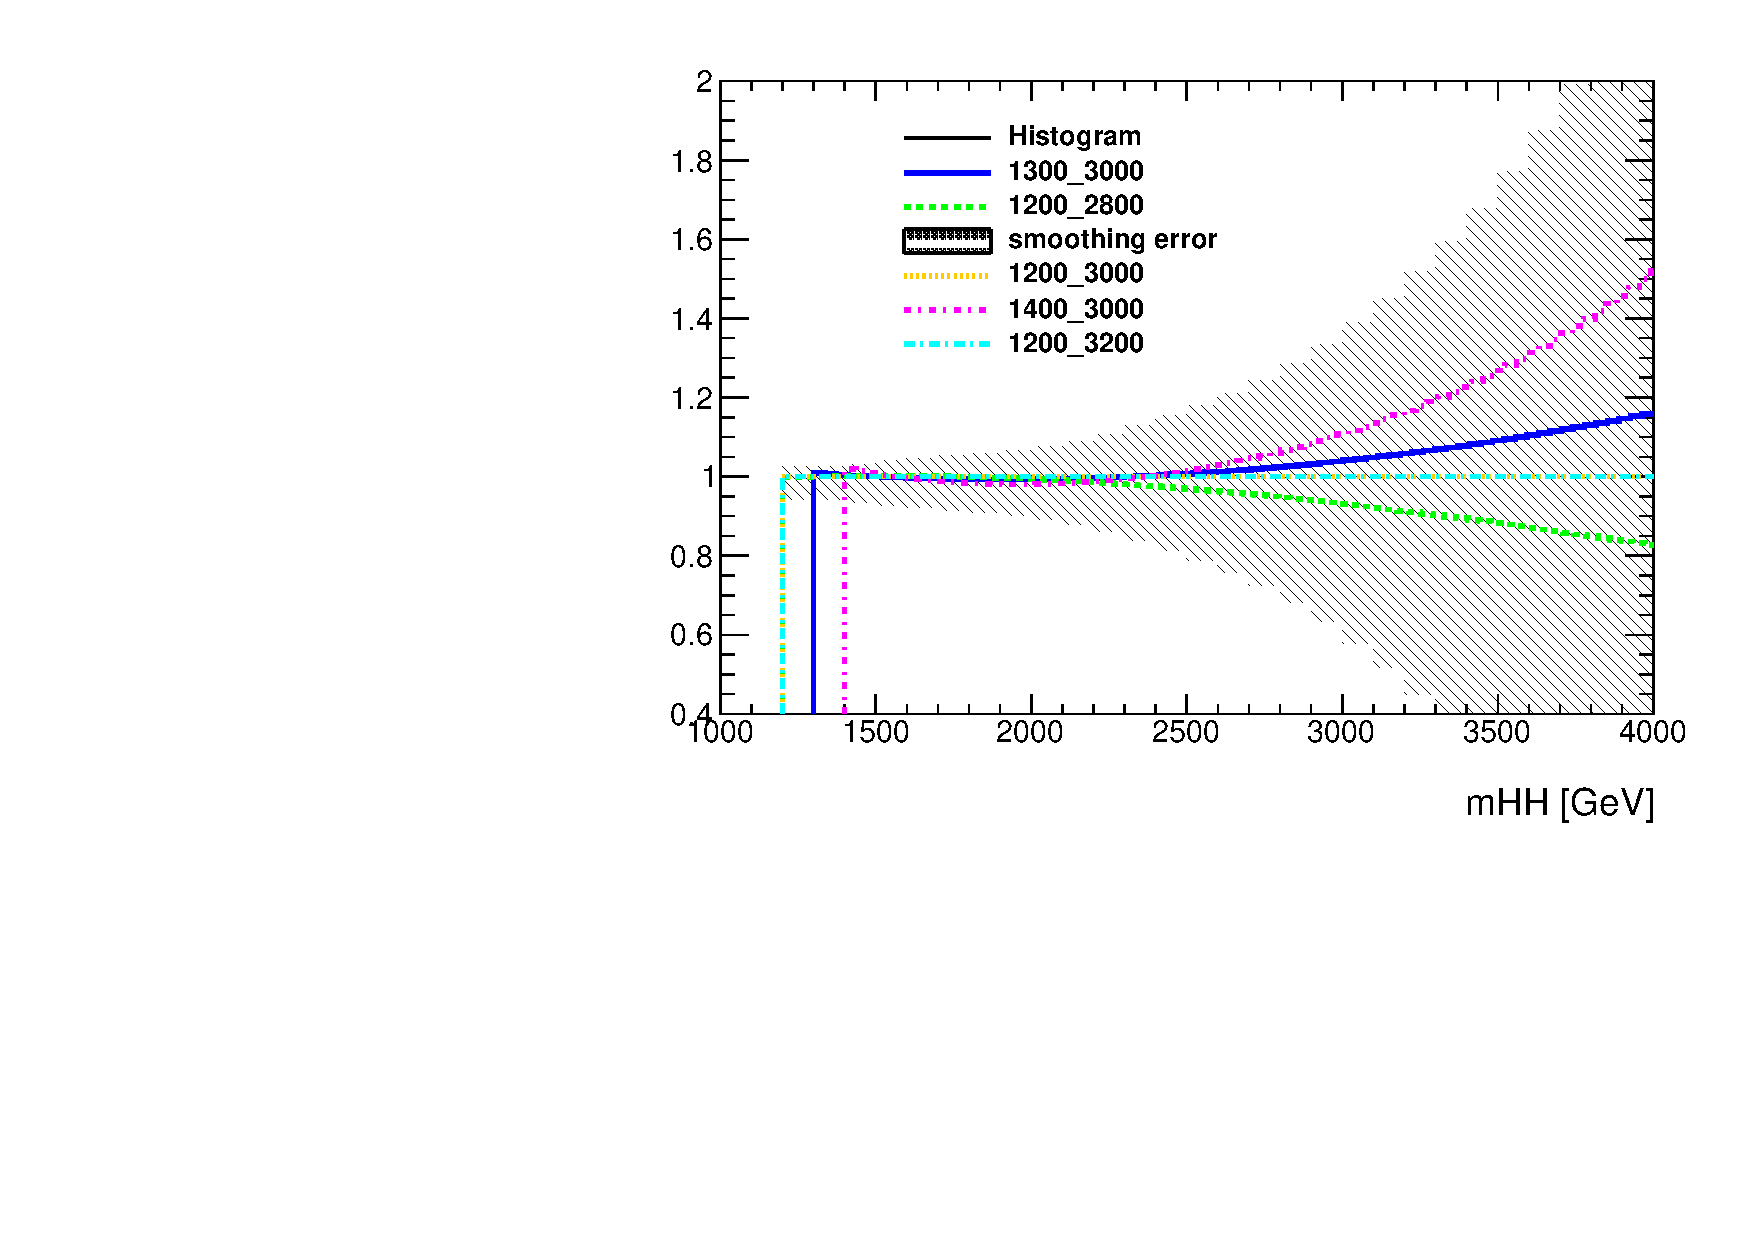
\includegraphics[width=0.31\textwidth,angle=-90]{figures/boosted/Syst_Smooth/smoothFuncRangeCompare_33_comp_ratio.pdf} \\
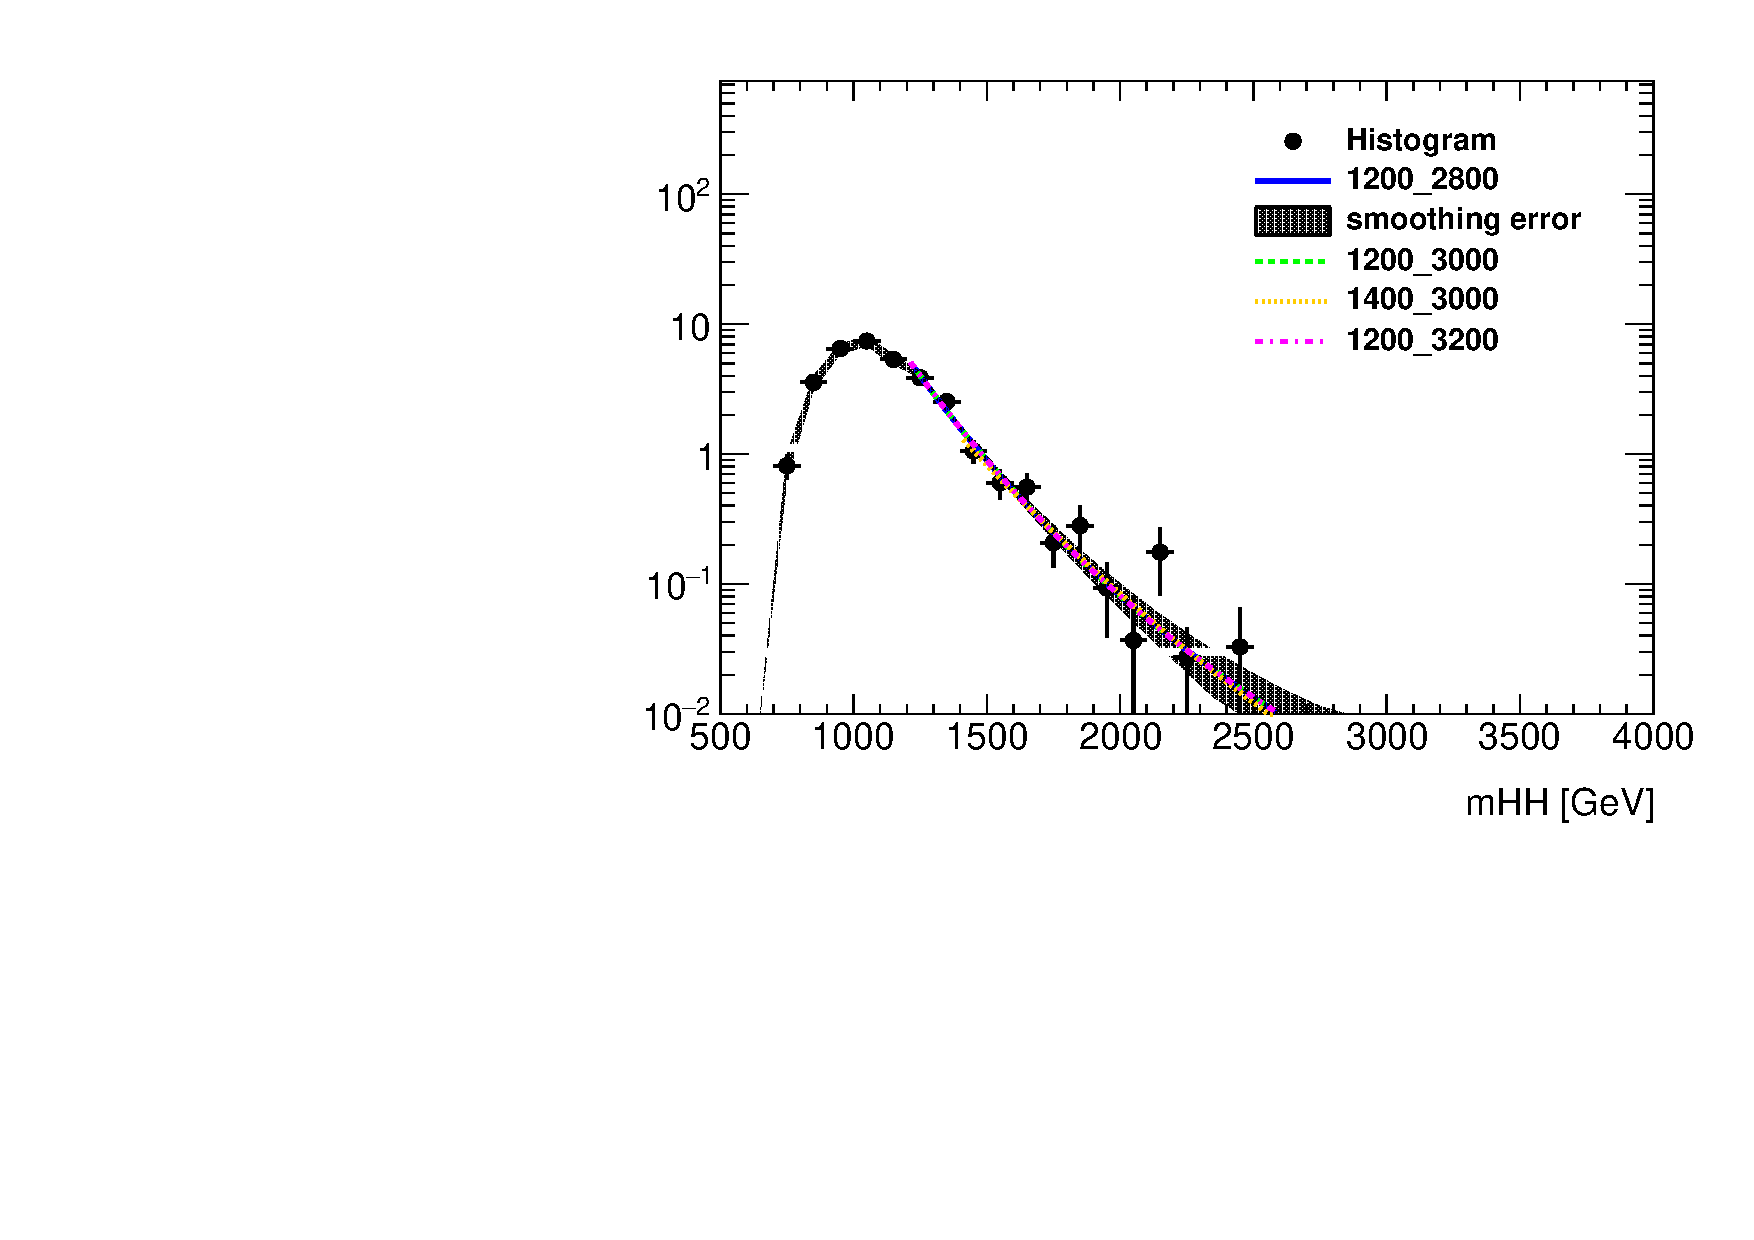
\includegraphics[width=0.31\textwidth,angle=-90]{figures/boosted/Syst_Smooth/smoothFuncRangeCompare_44_comp.pdf}
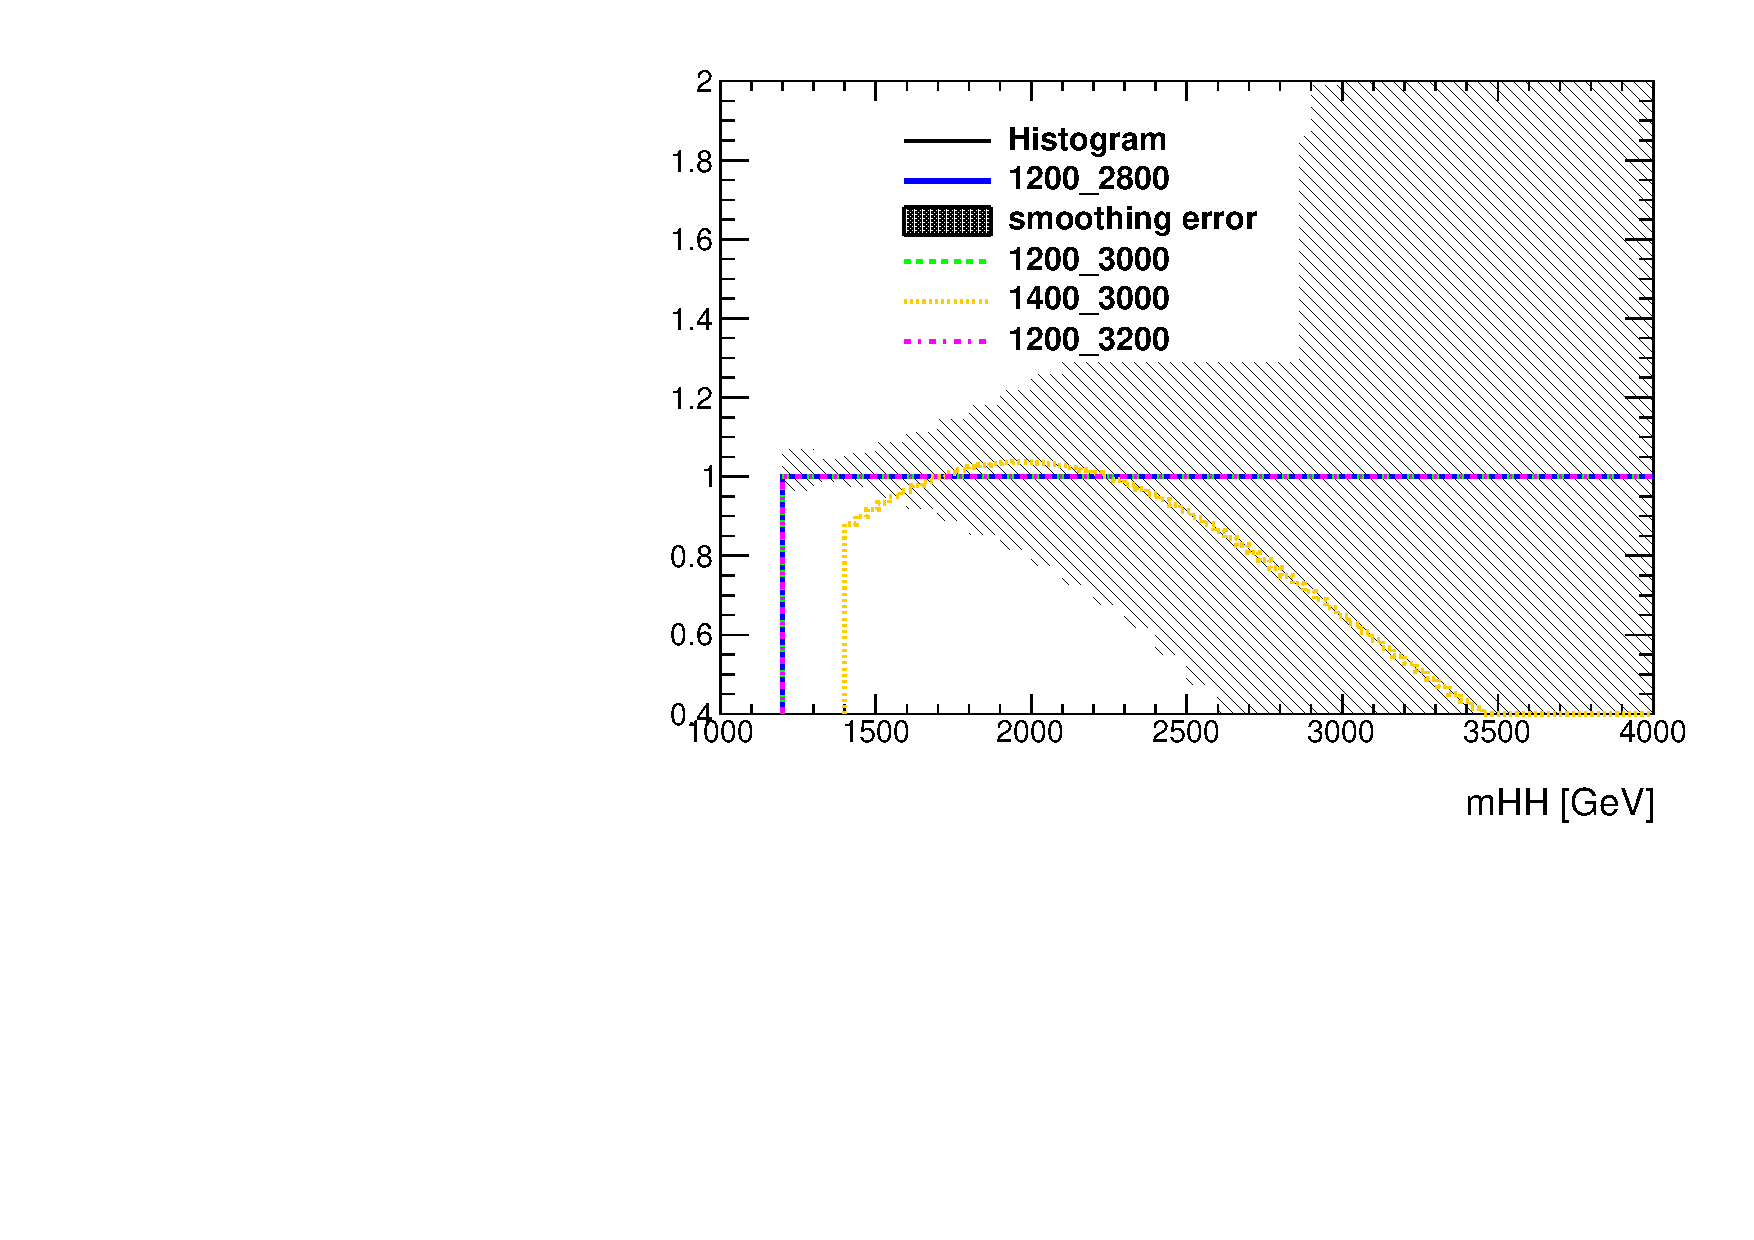
\includegraphics[width=0.31\textwidth,angle=-90]{figures/boosted/Syst_Smooth/smoothFuncRangeCompare_44_comp_ratio.pdf} \\
\caption{Dijet mass distribution SR prediction fit with several fit ranges (left) and the ratio of nominal to fits with different fit ranges (right)  for the 2b (top) 3b (middle) and 4b (bottom) samples. }
\label{fig:qcd_fit_range_sys_ratio-scaled}
\end{center}
\end{figure}

\paragraph{}
As a second test, we fit the $1/2b$ QCD prediction with a variety of other distributions which can show both power law behavior in the bulk of the distribution as well as longer tails.  The set of additional functions examined (labelled MJ1-MJ7) can be found in Table~\ref{tab:fit_funcs}, where $x = m_{JJ} / \sqrt{s}$.

\begin{table}[htbp!]
\begin{center} 
\begin{tabular}{  l | c}
Name & Functional Form \\
\hline
MJ1 (Dijet) & $f_{1}(x) = p_0 (1-x)^{p_1} x^{p_2}$ \\
MJ2 & $f_{2}(x) = p_0 (1-x)^{p_1} e^{p_2\ x^2}$ \\
MJ3 & $f_{3}(x) = p_0 (1-x)^{p_1} x^{p_2\ x}$ \\
MJ4 & $f_{4}(x) = p_0 (1-x)^{p_1} x^{p_2\ ln\ x}$ \\
MJ5 & $f_{5}(x) = p_0 (1-x)^{p_1} (1+x)^{p_2\ x}$ \\
MJ6 & $f_{6}(x) = p_0 (1-x)^{p_1} (1+x)^{p_2\ ln\ x}$ \\
MJ7 & $f_{7}(x) = \frac{p_0}{x} (1-x)^{p_1 - p_2\ ln\ x}$ \\
MJ8 & $f_{8}(x) = \frac{p_0}{x^2} (1-x)^{p_1 - p_2\ ln\ x}$ \\
\hline
\end{tabular}
\caption{Functions used to fit the QCD dijet mass distributions, where $x = m_{JJ} / \sqrt{s}$.}
\label{tab:fit_funcs}
\end{center}
\end{table}

\paragraph{}
Figure~\ref{fig:qcd_fit_funcs_sys} shows the fits to the QCD prediction in the 4/3/2b  signal regions, and the nominal dijet fit, as well as the ratios of the nominal fit to that of the additional functions.  The maximum per bin deviation is taken as the shape systematic, separately for the $4/3/2bs$ SRs.

\paragraph{}
As before, fits in which the fit $\chi^2$ probability was less than 0.1\%,  or in which the fit integrals between 1500-2000 GeV, 2000-2500 GeV, or $>$2500 GeV were not in agreement with the original 0b distribution within a factor of 2 or 0.5, were not used to estimate the uncertainty.  The aforementioned checks ensure that we do not use poor fits of the 0b distribution to estimate the uncertainty.

\begin{figure}[htbp!]
\begin{center}
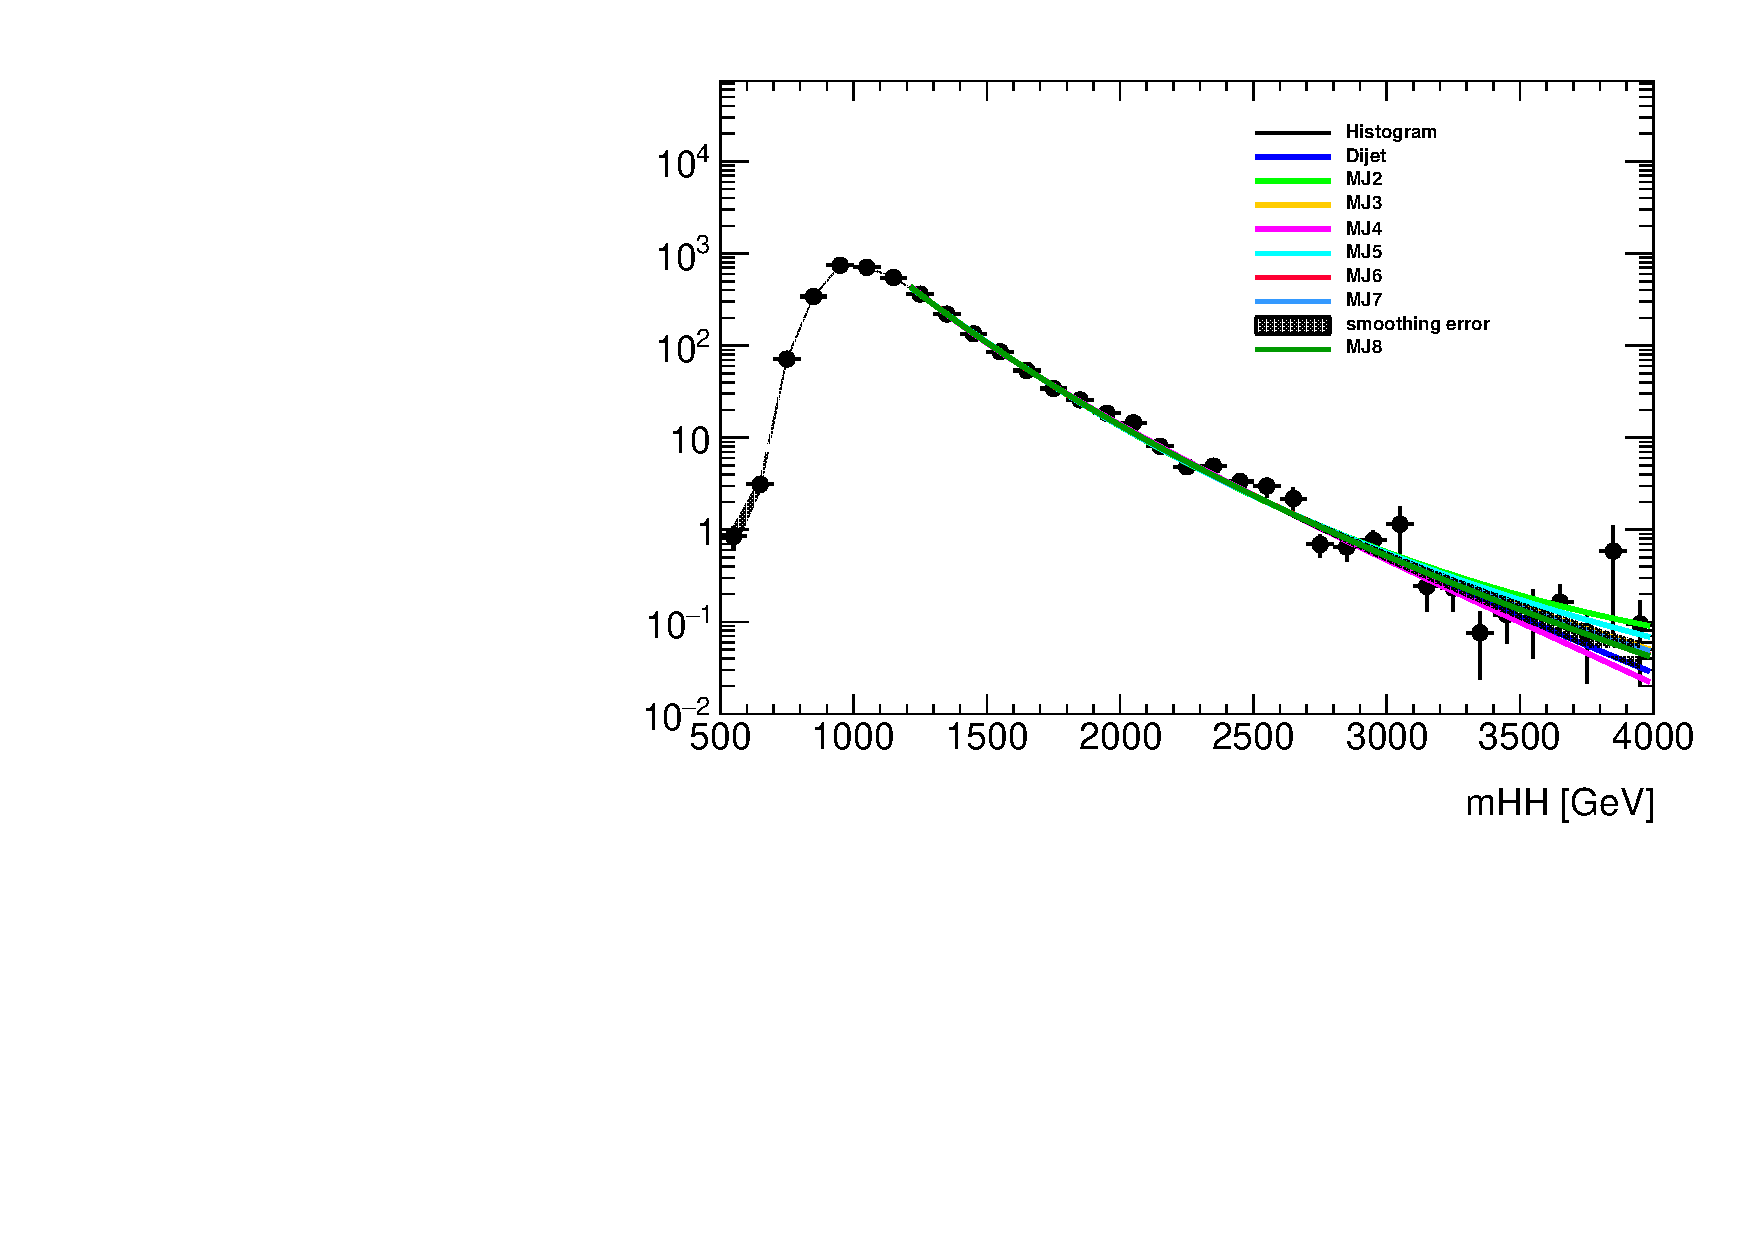
\includegraphics[width=0.31\textwidth,angle=-90]{figures/boosted/Syst_Smooth/smoothFuncCompare_22_comp.pdf}
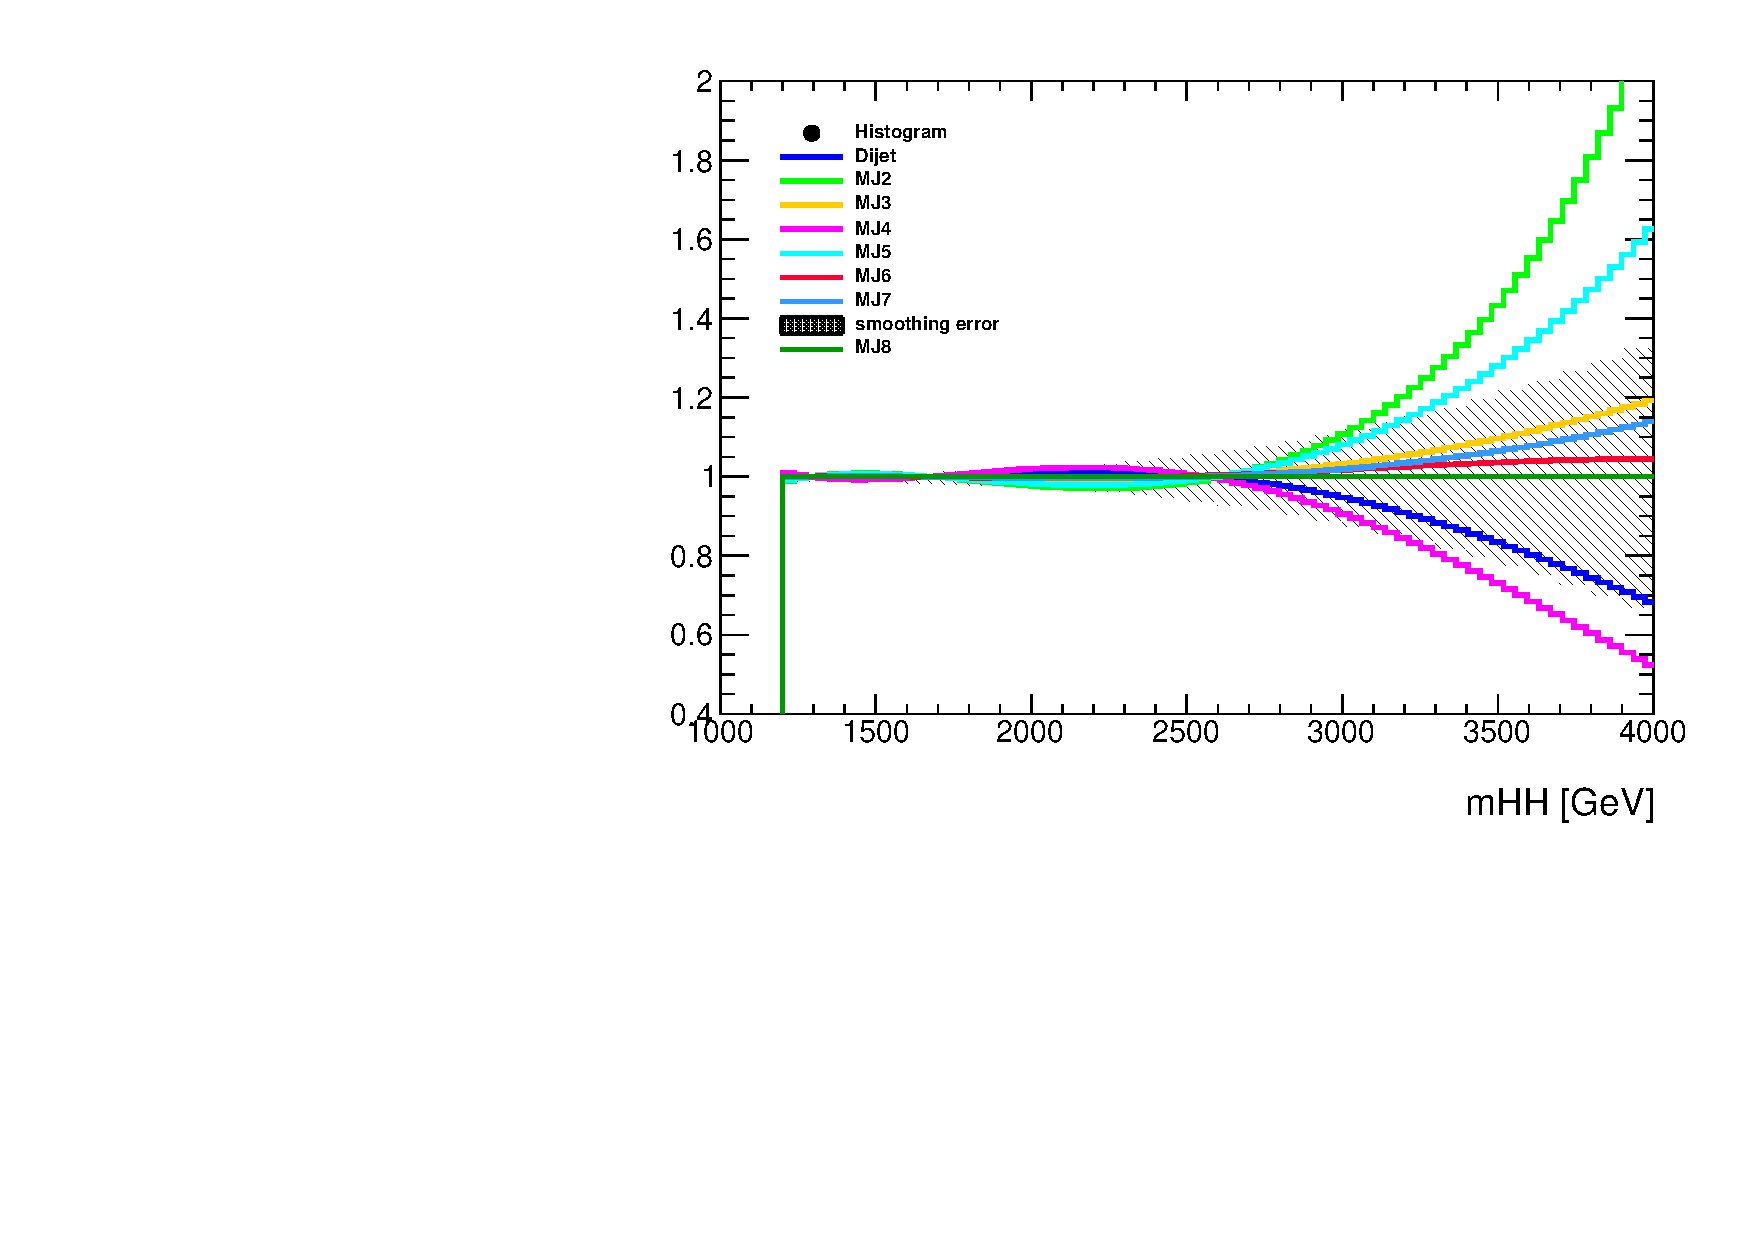
\includegraphics[width=0.31\textwidth,angle=-90]{figures/boosted/Syst_Smooth/smoothFuncCompare_22_comp_ratio.pdf} \\
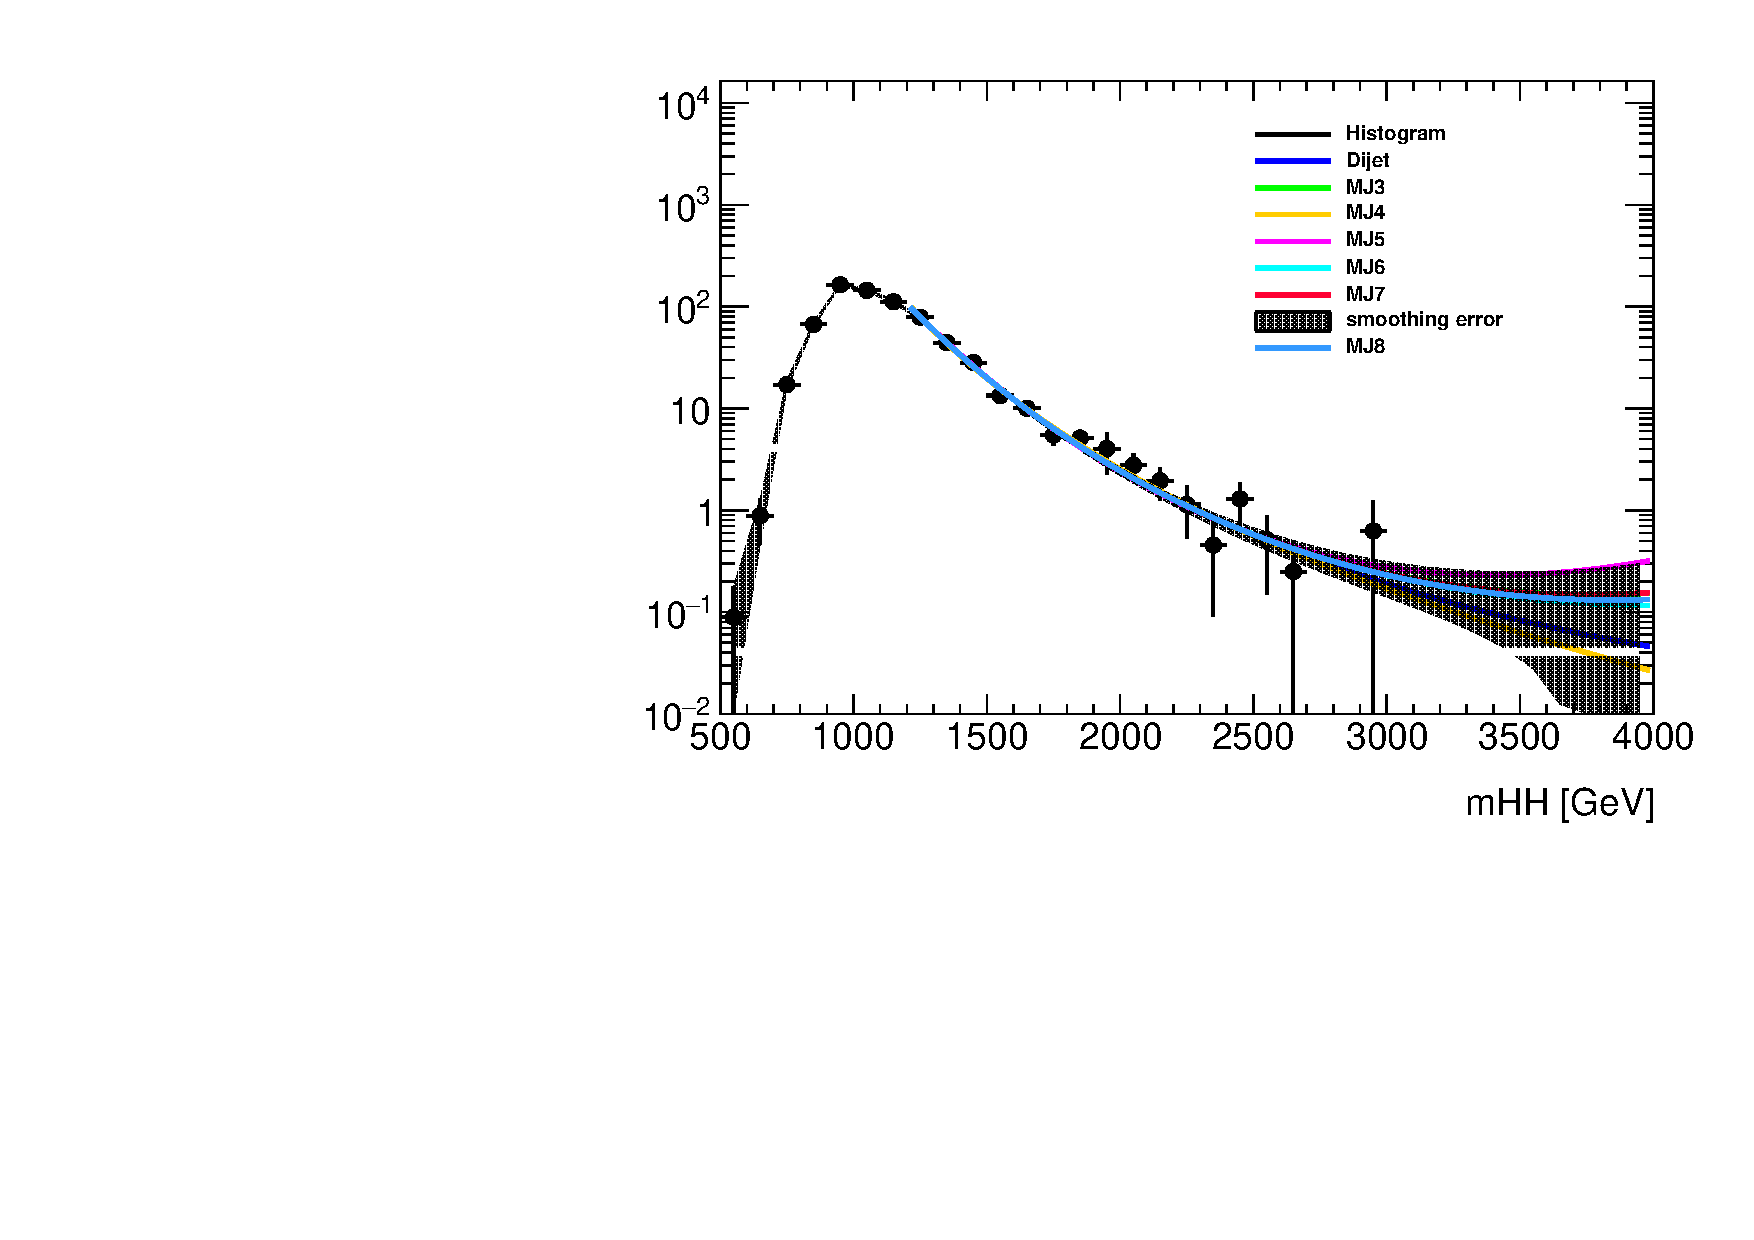
\includegraphics[width=0.31\textwidth,angle=-90]{figures/boosted/Syst_Smooth/smoothFuncCompare_33_comp.pdf}
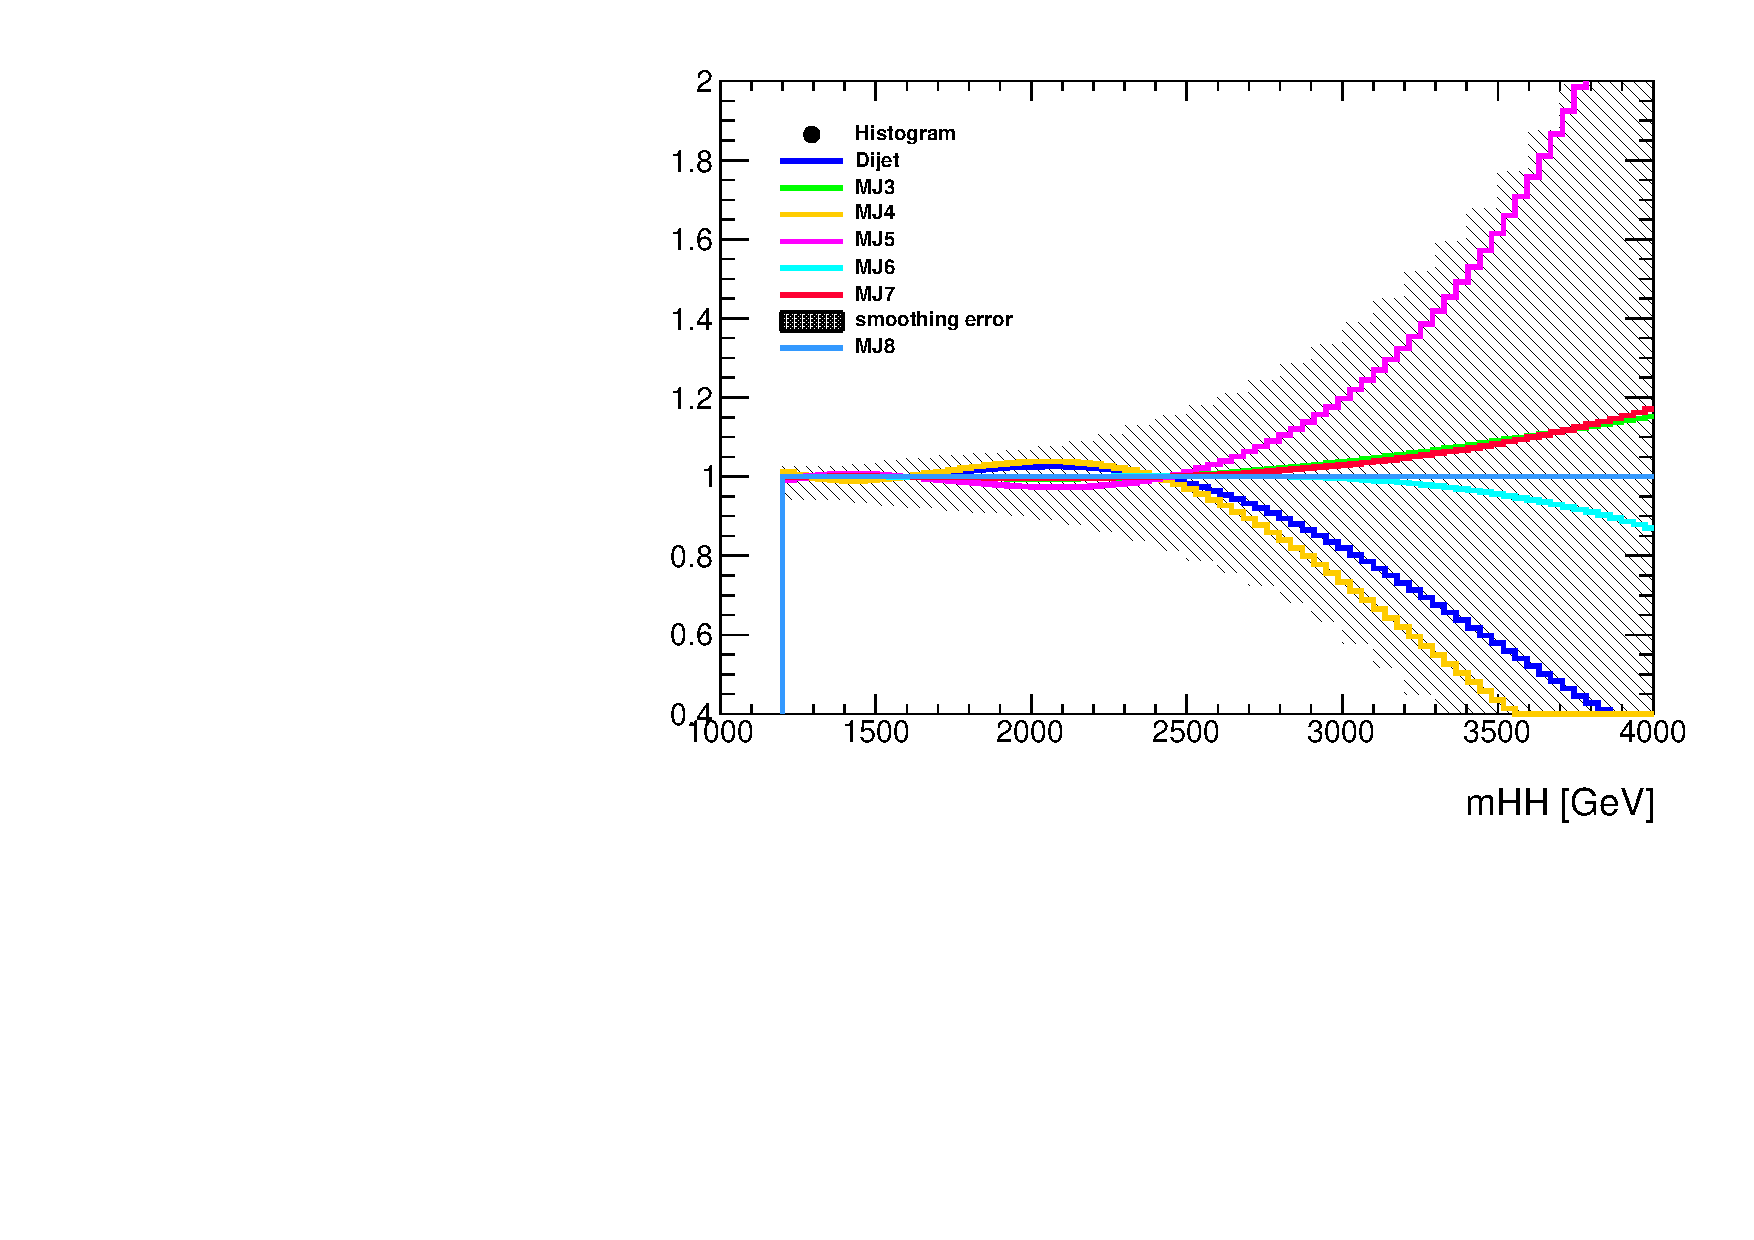
\includegraphics[width=0.31\textwidth,angle=-90]{figures/boosted/Syst_Smooth/smoothFuncCompare_33_comp_ratio.pdf} \\
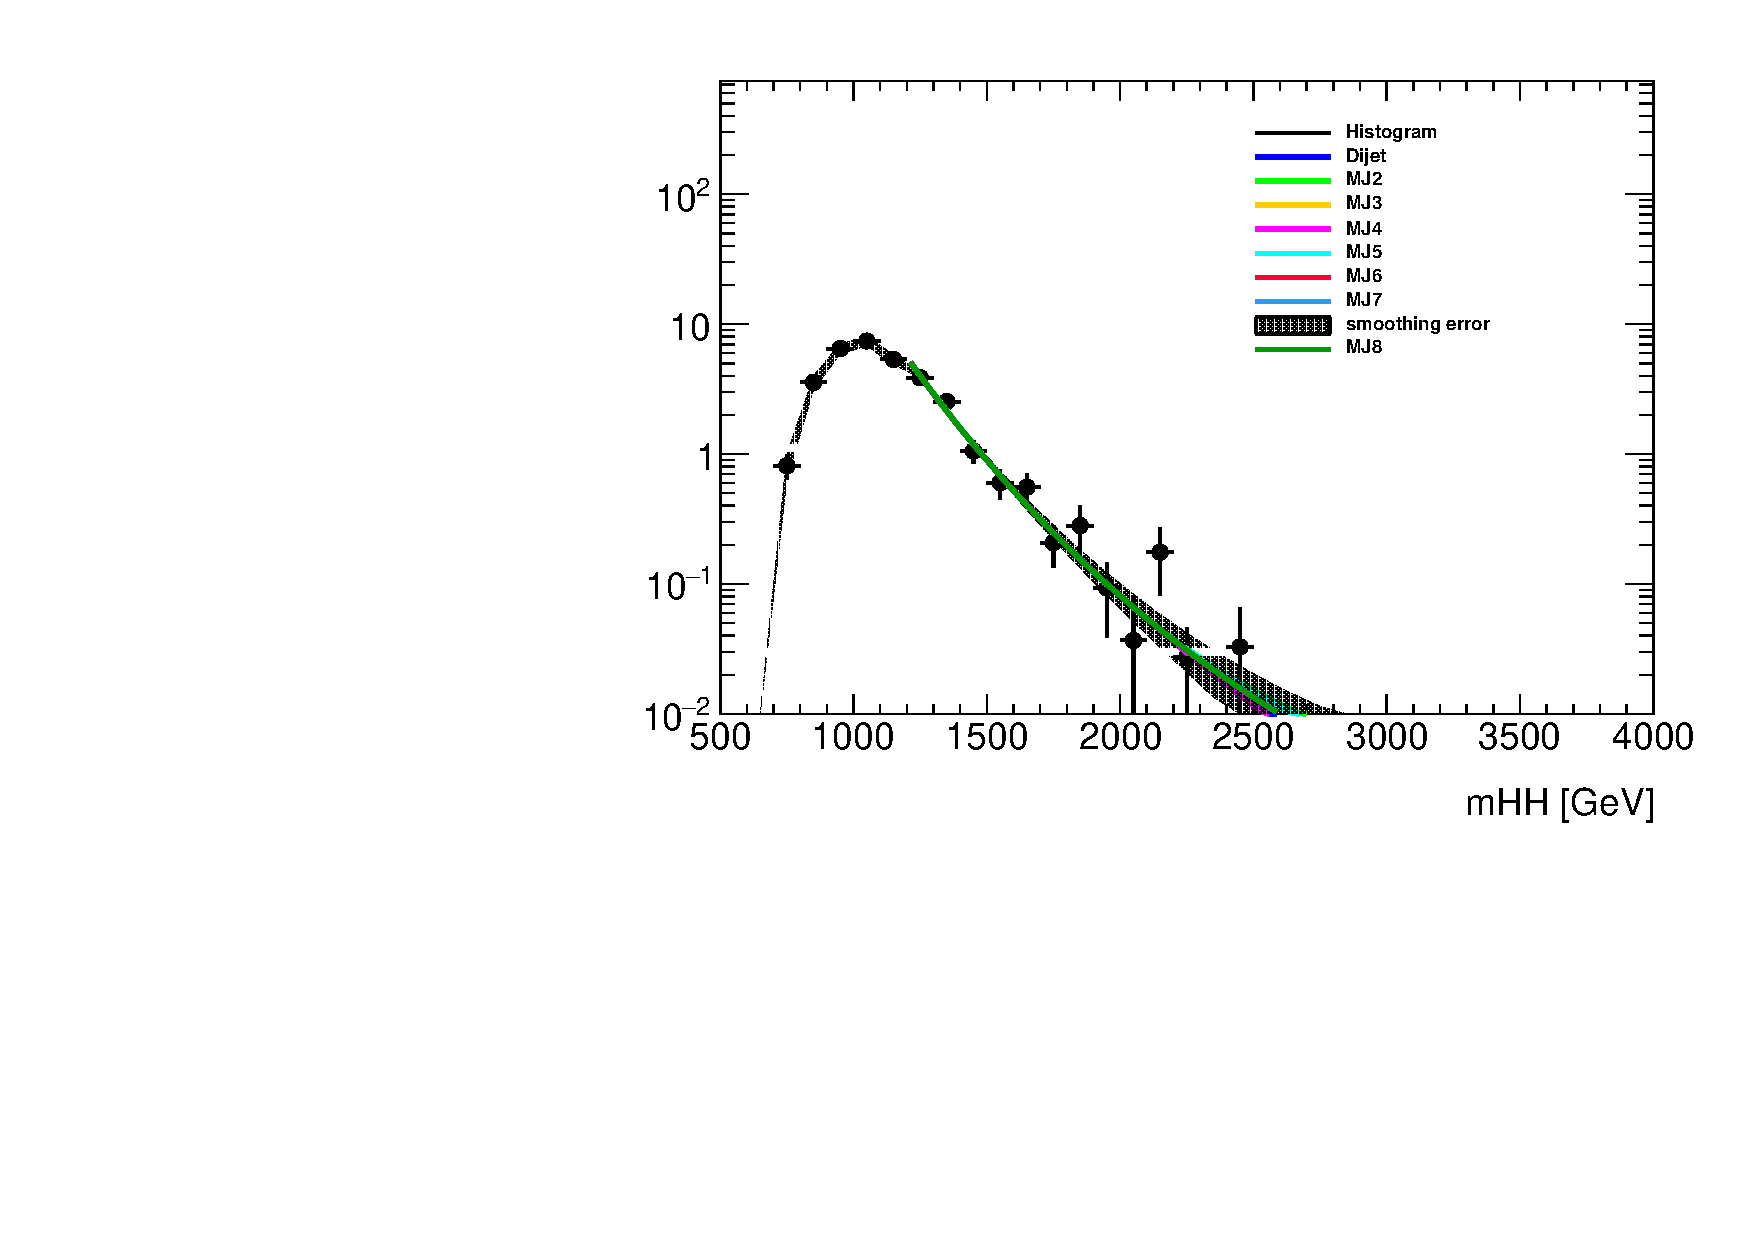
\includegraphics[width=0.31\textwidth,angle=-90]{figures/boosted/Syst_Smooth/smoothFuncCompare_44_comp.pdf}
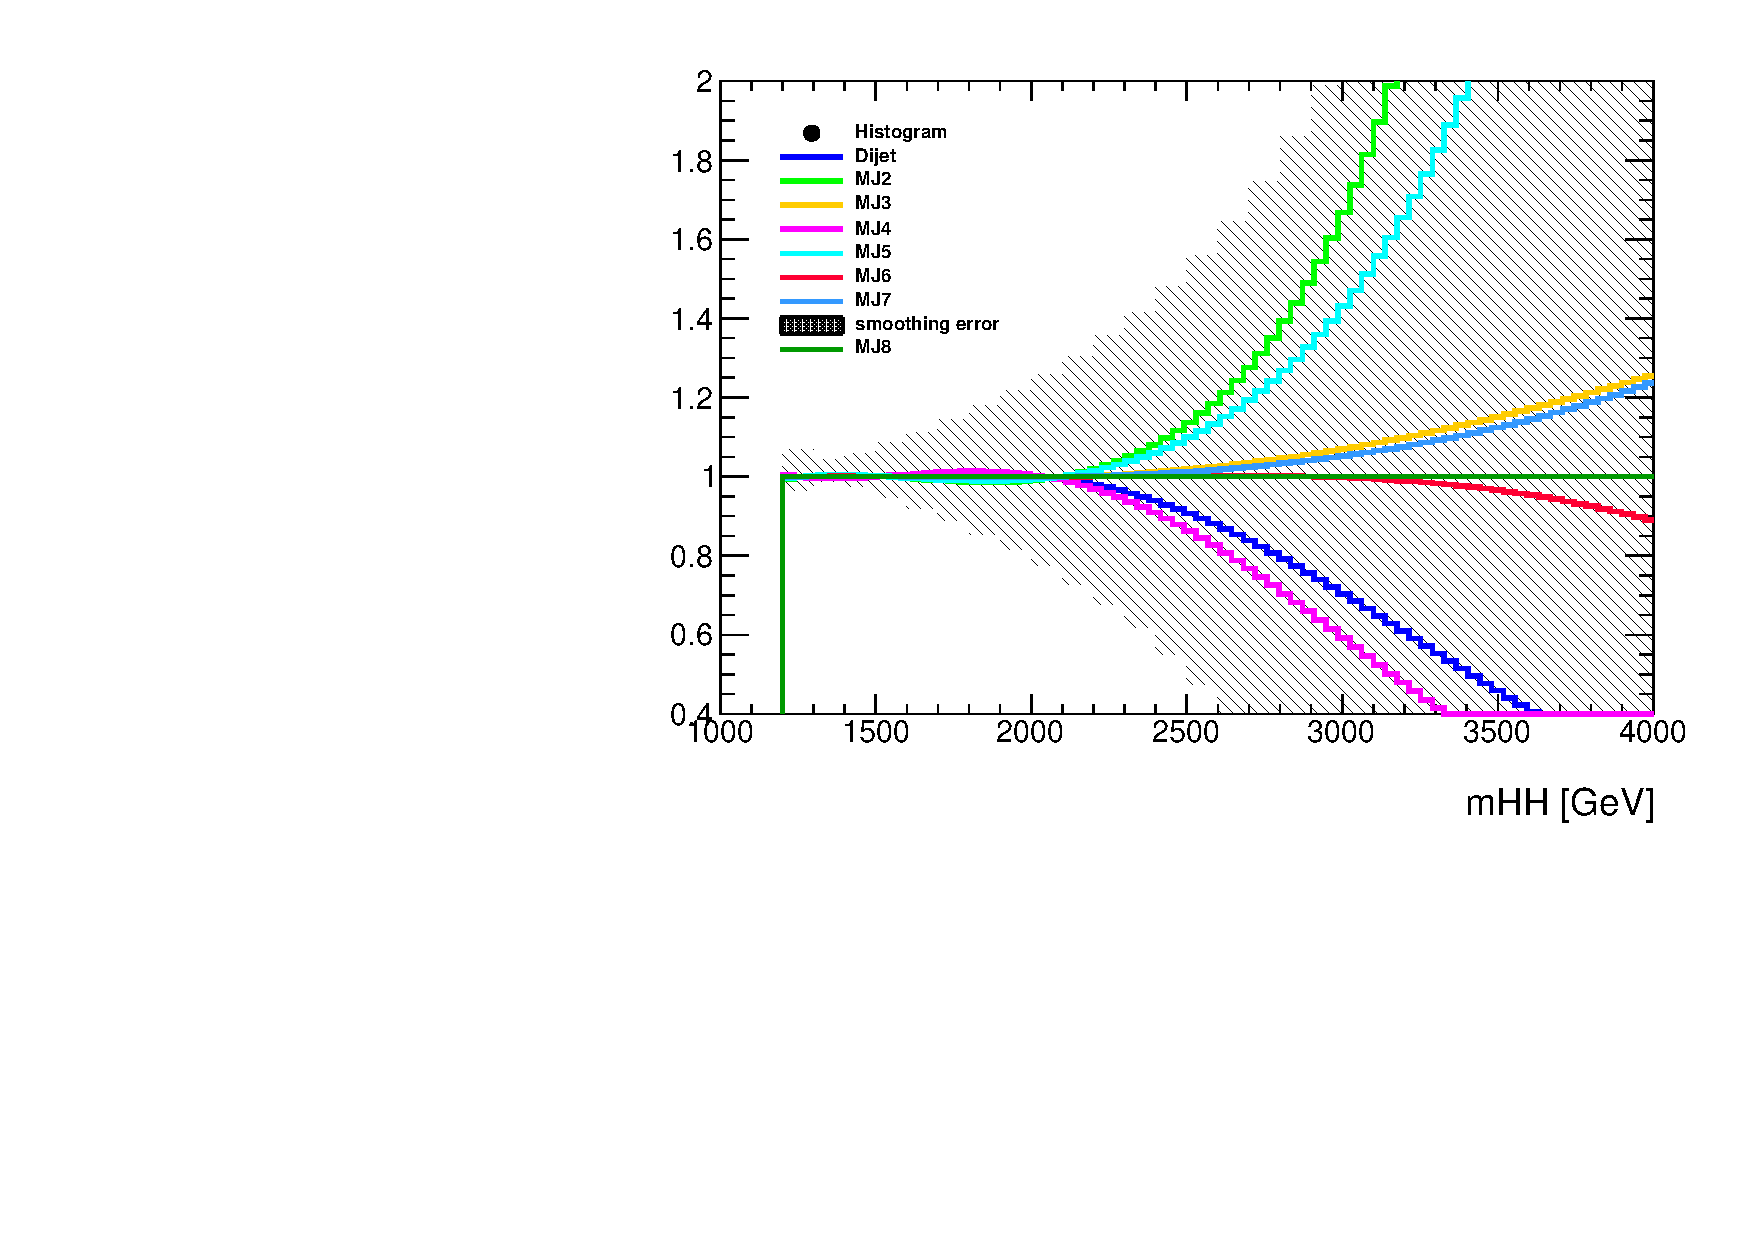
\includegraphics[width=0.31\textwidth,angle=-90]{figures/boosted/Syst_Smooth/smoothFuncCompare_44_comp_ratio.pdf} \\
\caption{ Dijet mass distribution SR prediction fit with several fit functions (left) and the ratio of nominal to fits with different fit functions (right)  for the 2b (top) 3b (middle) and 4b (bottom) samples. The additional fit functions are from Table~\ref{tab:fit_funcs}.}
\label{fig:qcd_fit_funcs_sys}
\end{center}
\end{figure}

%%%%%%%%%%%%%%%%%%%%%%%%%%%%%%%%%%%%%%%%%%%%%%%%%%%%%%%%%%%%%%%%%%%%%%%
%%%%%%%%%%%%%%%%%%%%%%%%%%%%%%%%%%%%%%%%%%%%%%%%%%%%%%%%%%%%%%%%%%%%%%%

\subsection{Summary of systematics}
\label{sec:boosted-systematics-numbers}

\paragraph{}
Table~\ref{tab:summary-systematics-4b} shows the percent impact of systematics used in this analysis on the backgrounds yields and on the expected yields for RSG $c=1.0$ signals in the $4b$ signal region. The correspondent values are shown for the $3b$ signal region in Table ~\ref{tab:summary-systematics-3b}, and are shown for the $2bs$ signal region in Table ~\ref{tab:summary-systematics-2b}.

\paragraph{}
The ``Background Normalization Fit'' uncertainty comes from summing in quadrature the independent uncertainty components calculated from the correlated statistical errors of \muqcd and \alphatt. 
The ``QCD Non-Closure in CR'' systematic is derived as the maximum of (a) difference between the predicted and observed 4b/3b/2bs QCD yields in the control region, (b) the fractional change in SR predictions from varying the CR and SB definitions. 
Both options gave similar sized uncertainties, but the uncertainty from the CR/SB variations was found to be larger. 
All these uncertainties are summed in quarature and shown in the ``Bkg Est'' row in the table.

\paragraph{}
The remaining systematics not listed in this table, as they do not impact the yield, including uncertainties on the shape of the QCD and \ttbar\ backgrounds in the signal region, and the uncertainties from the smoothing / extrapolation procedure.

\paragraph{}
The size of the Monte Carlo modeling systematics on the RSG c=1.0 signal yield as a function of the signal mass can be found in Figure~\ref{fig:signal_syst_summary}. 
These uncertainties have a similar impact on the other signals. The largest uncertainty in the $4b$ and $2b$ signal region is from $b$-tagging, followed by the JMR uncertainty. 
In the $3b$ signal region, although $b$-tagging systematics is still one of the largest uncertainty, it has been much reduced compared to $4b$ region, as discussed in Section~\ref{sec:b-tagging-unc}. 
Then the jet mass scale and resolution are the largest uncertainties following b-tagging. 

\begin{table}[htbp!]
\scriptsize
\begin{center}
\caption{Percent impact of the dominant systematics on the  background acceptance
         and on the signal acceptance of RS $c=1.0$ graviton predictions in the $4b$ signal region.}
\begin{footnotesize} 
\begin{tabular}{c|c|c|c|c|c|c} 
FourTag & totalbkg & qcd & ttbar & RSG1 1000 & RSG1 2000 & RSG1 3000 \\ 
\hline\hline 
JER & 0.45 & 0.27 & 3.98 & 2.44 & 1.07 & 0.67\\ 
JMR & 7.9 & 10.35 & 39.95 & 12.33 & 13.16 & 15.08\\ 
Top &  -  &  -  &  -  &  -  &  -  &  - \\ 
JES/JMS & 1.32 & 1.49 & 24.36 & 5.18 & 3.72 & 5.62\\ 
Bkg Est & 15.67 & 18.19 & 67.82 &  -  &  -  &  - \\ 
b-tag SF & 1.11 & 0.79 & 18.85 & 18.34 & 28.11 & 27.73\\ 
\hline 
Total Sys & 17.64 & 21.0 & 84.62 & 22.83 & 31.28 & 32.07\\ 
\hline 
Stat & 3.13 & 3.29 & 2.47 & 1.97 & 1.63 & 4.9\\ 
\hline 
Estimated Events & 34.59 & 32.91 & 1.68 & 10.07 & 0.25 & 0.0016\\ 
\hline\hline 
\end{tabular} 
\end{footnotesize} 
\newline 

\label{tab:summary-systematics-4b}
\end{center}
\end{table}

\begin{table}[htbp!]
\scriptsize
\begin{center}
\caption{Percent impact of the dominant systematics on the  background acceptance
         and on the signal acceptance of RS $c=1.0$ graviton predictions in the $3b$ signal region.}
\begin{footnotesize} 
\begin{tabular}{c|c|c|c|c|c|c} 
ThreeTag & totalbkg & qcd & ttbar & RSG1 1000 & RSG1 2000 & RSG1 3000 \\ 
\hline\hline 
JER & 1.38 & 3.52 & 17.5 & 1.41 & 0.93 & 1.08\\ 
JMR & 1.35 & 4.26 & 24.38 & 14.3 & 12.33 & 15.53\\ 
Top &  -  &  -  &  -  &  -  &  -  &  - \\ 
JES/JMS & 2.03 & 1.26 & 26.22 & 5.19 & 1.94 & 6.35\\ 
Bkg Est & 4.84 & 5.62 & 9.45 &  -  &  -  &  - \\ 
b-tag SF & 0.47 & 0.53 & 8.45 & 2.45 & 2.01 & 9.27\\ 
\hline 
Total Sys & 5.61 & 8.0 & 41.82 & 15.47 & 12.68 & 19.2\\ 
\hline 
Stat & 1.32 & 1.44 & 2.47 & 1.26 & 1.0 & 1.83\\ 
\hline 
Estimated Events & 780.89 & 701.52 & 79.38 & 26.0 & 0.76 & 0.013\\ 
\hline\hline 
\end{tabular} 
\end{footnotesize} 
\newline 

\label{tab:summary-systematics-3b}
\end{center}
\end{table}

\begin{table}[htbp!]
\scriptsize
\begin{center}
\caption{Percent impact of the dominant systematics on the  background acceptance
         and on the signal acceptance of RS $c=1.0$ graviton predictions in the $2bs$ signal region.}
\begin{footnotesize} 
\begin{tabular}{c|c|c|c|c|c|c} 
TwoTag split & totalbkg & qcd & ttbar & RSG1 1000 & RSG1 2000 & RSG1 3000 \\ 
\hline\hline 
JER & 0.25 & 0.48 & 3.14 & 1.18 & 0.74 & 0.5\\ 
JMR & 0.52 & 1.73 & 9.43 & 10.96 & 12.3 & 13.05\\ 
Top & 4.82 & 6.98 & 26.63 &  -  &  -  &  - \\ 
JES/JMS & 0.43 & 1.67 & 7.17 & 6.72 & 1.69 & 3.44\\ 
Bkg Est & 2.76 & 3.38 & 2.35 &  -  &  -  &  - \\ 
b-tag SF & 0.83 & 1.43 & 1.82 & 19.28 & 27.36 & 2.7\\ 
\hline 
Total Sys & 5.66 & 8.26 & 29.46 & 23.2 & 30.05 & 13.77\\ 
\hline 
Stat & 0.6 & 0.42 & 2.48 & 2.0 & 1.2 & 1.07\\ 
\hline 
Estimated Events & 4252.44 & 3393.74 & 858.7 & 10.87 & 0.6 & 0.039\\ 
\hline\hline 
\end{tabular} 
\end{footnotesize} 
\newline 

\label{tab:summary-systematics-2b}
\end{center}
\end{table}

\begin{figure}[htbp!]
\begin{center}
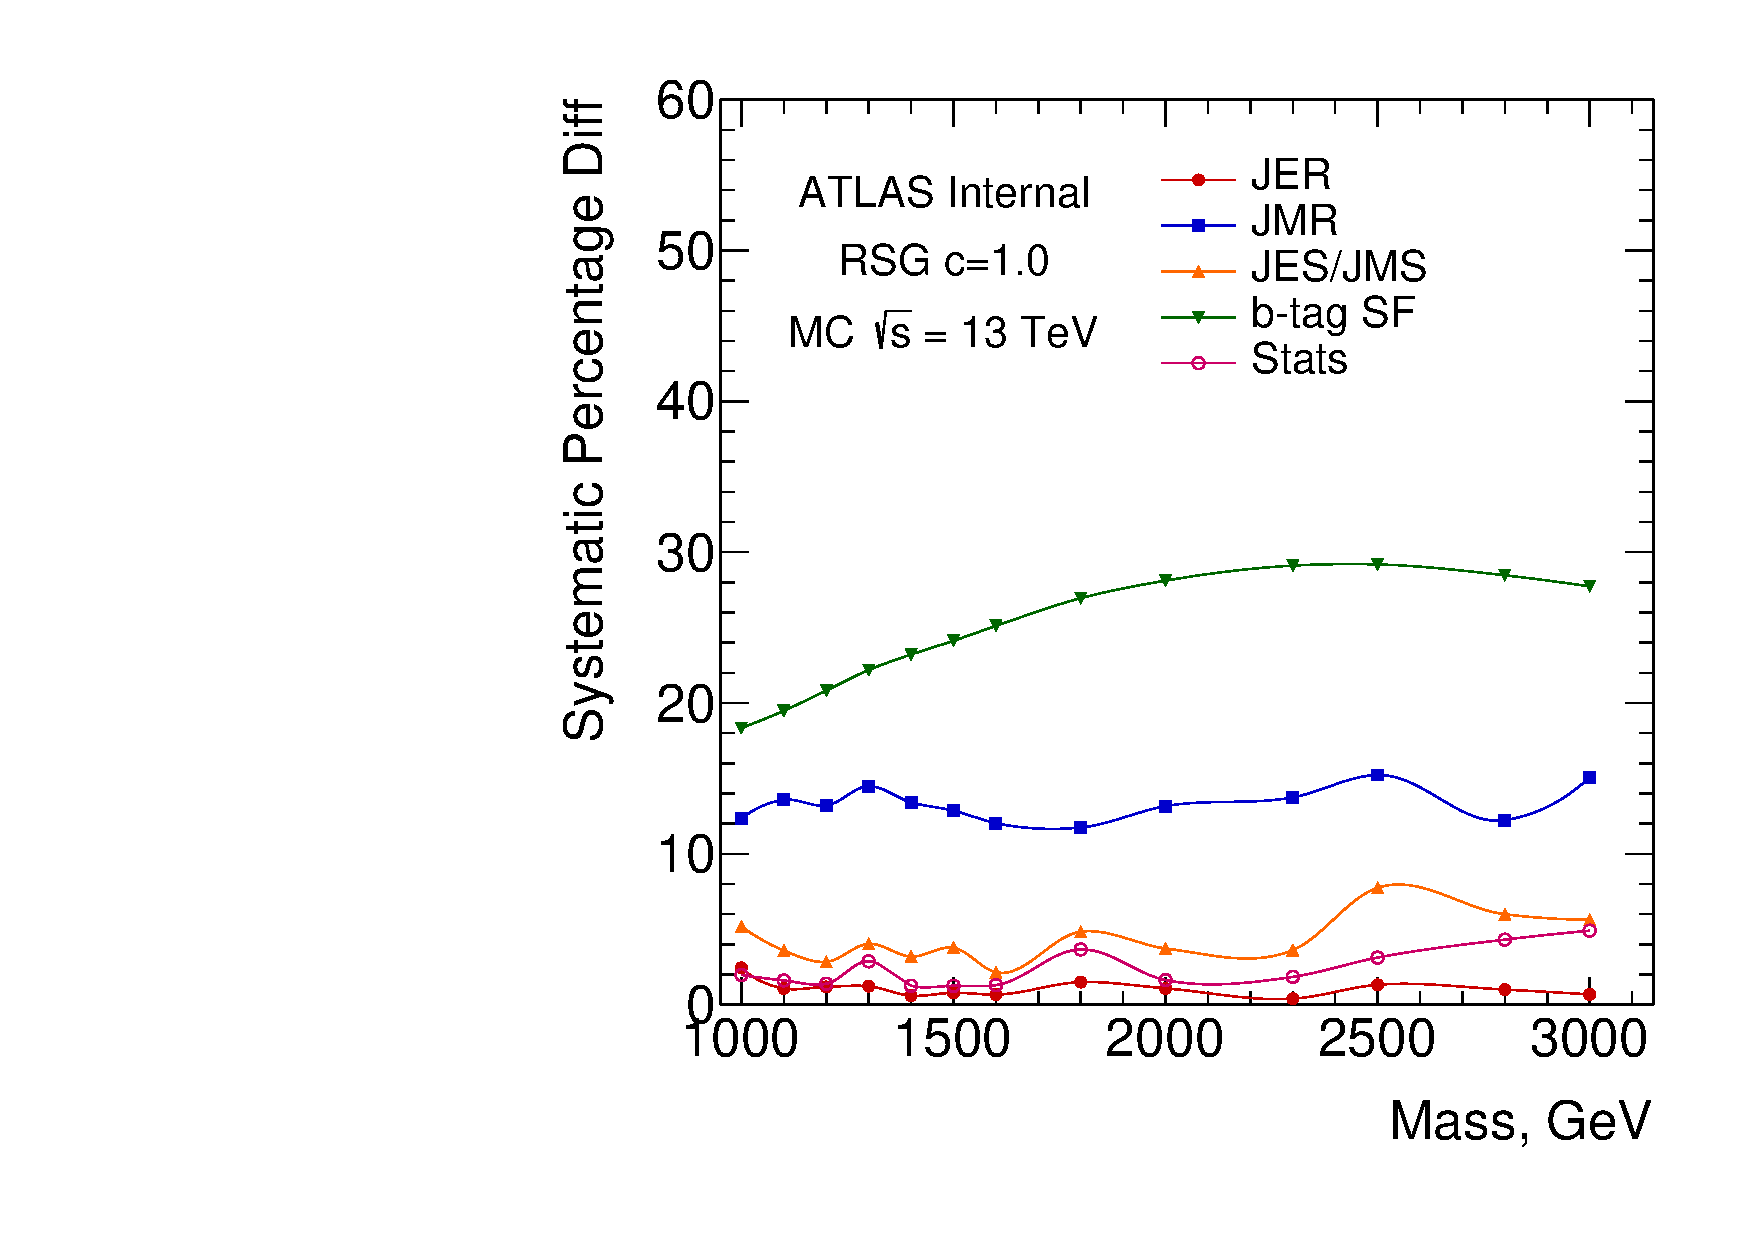
\includegraphics[width=0.31\textwidth,angle=-90]{figures/boosted/Syst_MC/FourTag_RSG_syst.pdf}
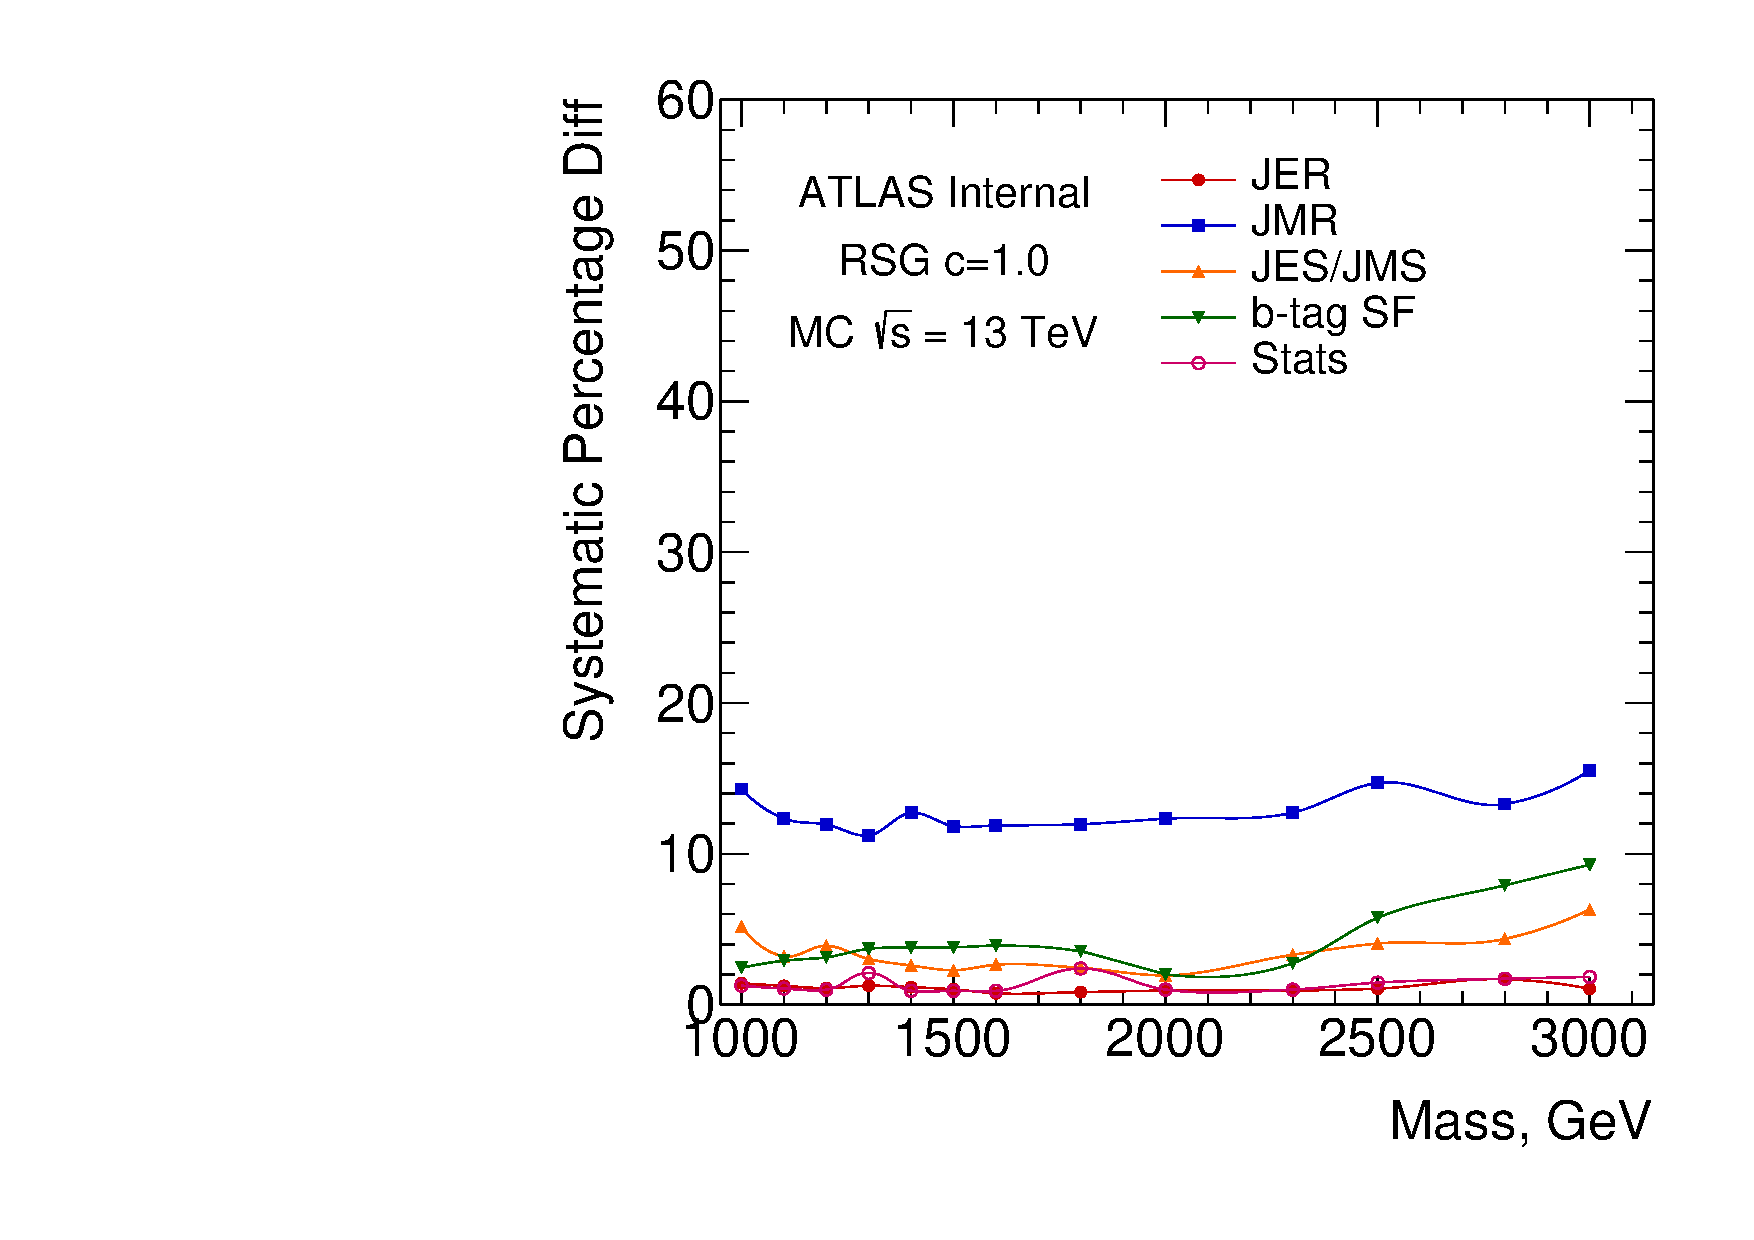
\includegraphics[width=0.31\textwidth,angle=-90]{figures/boosted/Syst_MC/ThreeTag_RSG_syst.pdf}
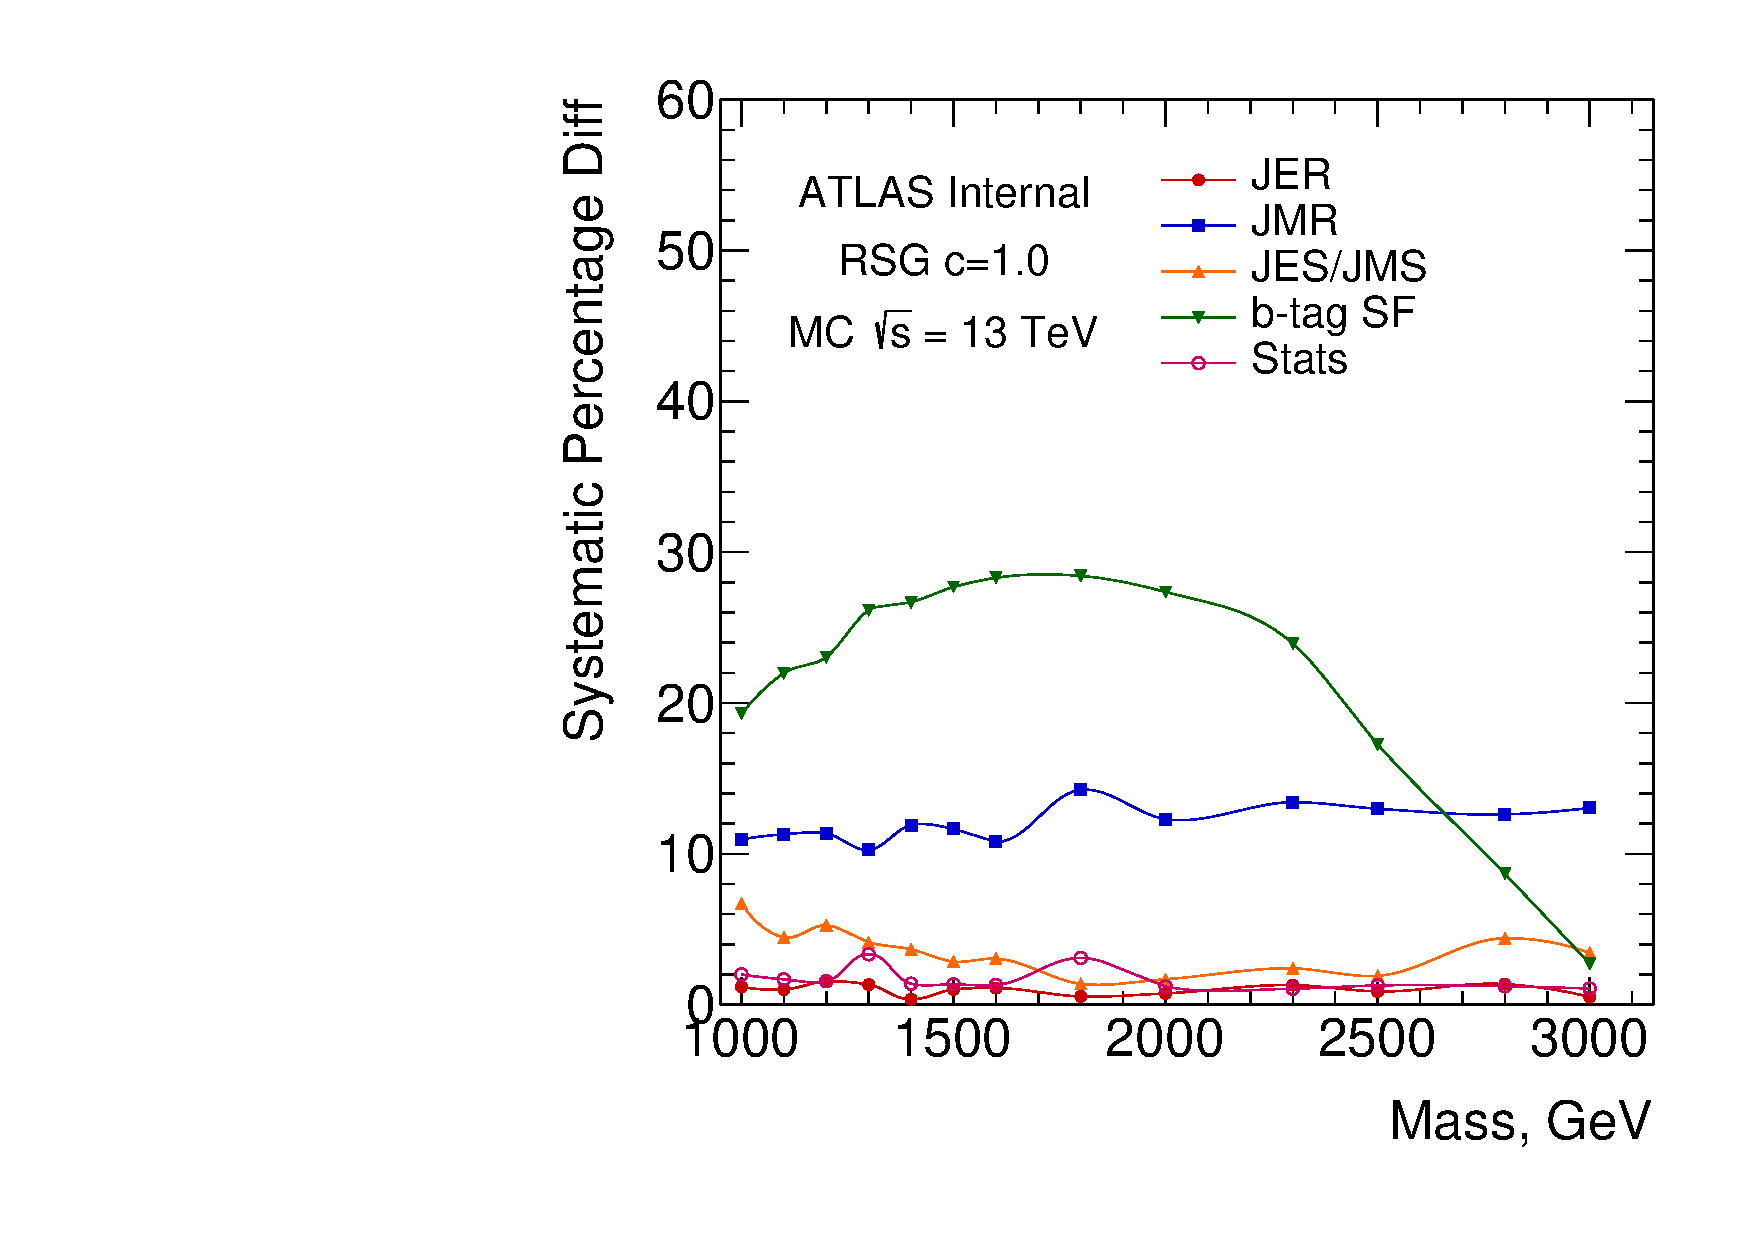
\includegraphics[width=0.31\textwidth,angle=-90]{figures/boosted/Syst_MC/TwoTag_split_RSG_syst.pdf}
\caption{Impact of each systematic on the signal prediction as a function of the signal mass, in the $4b$ (left) and $3b$ (middle) and $2bs$ signal regions.}
\label{fig:signal_syst_summary}
\end{center}
\end{figure}

\paragraph{}
The final background prediction of scaled \mtwoJ along with total uncertainties can be found in Figure~\ref{fig:FinalBkg_sys-4b-pole}, ~\ref{fig:FinalBkg_sys-3b-pole}, and ~\ref{fig:FinalBkg_sys-2b-pole}.

\begin{figure}
\begin{center}
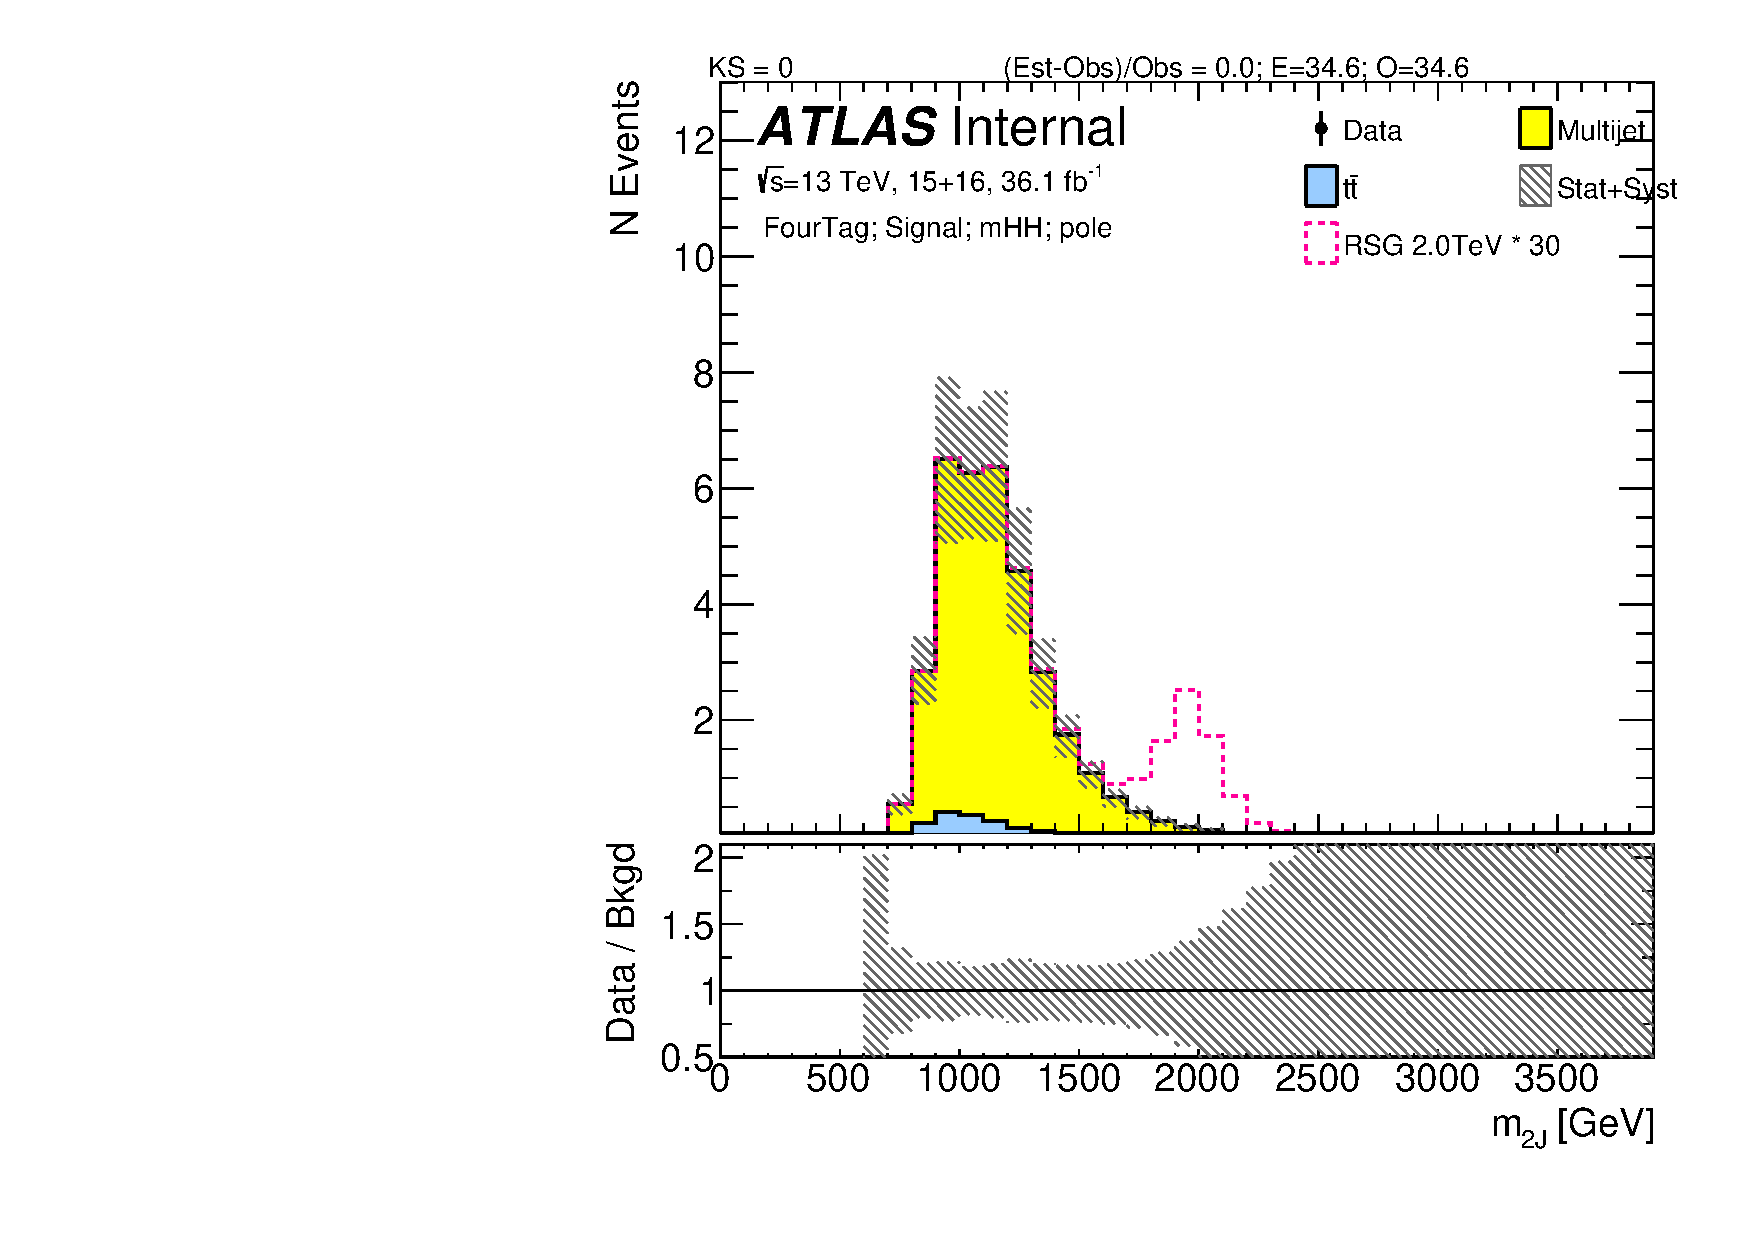
\includegraphics[width=0.48\textwidth,angle=-90]{figures/boosted/Signal_Syst/Moriond_bkg_9_FourTag_Signal_mHH_pole_blind.pdf}
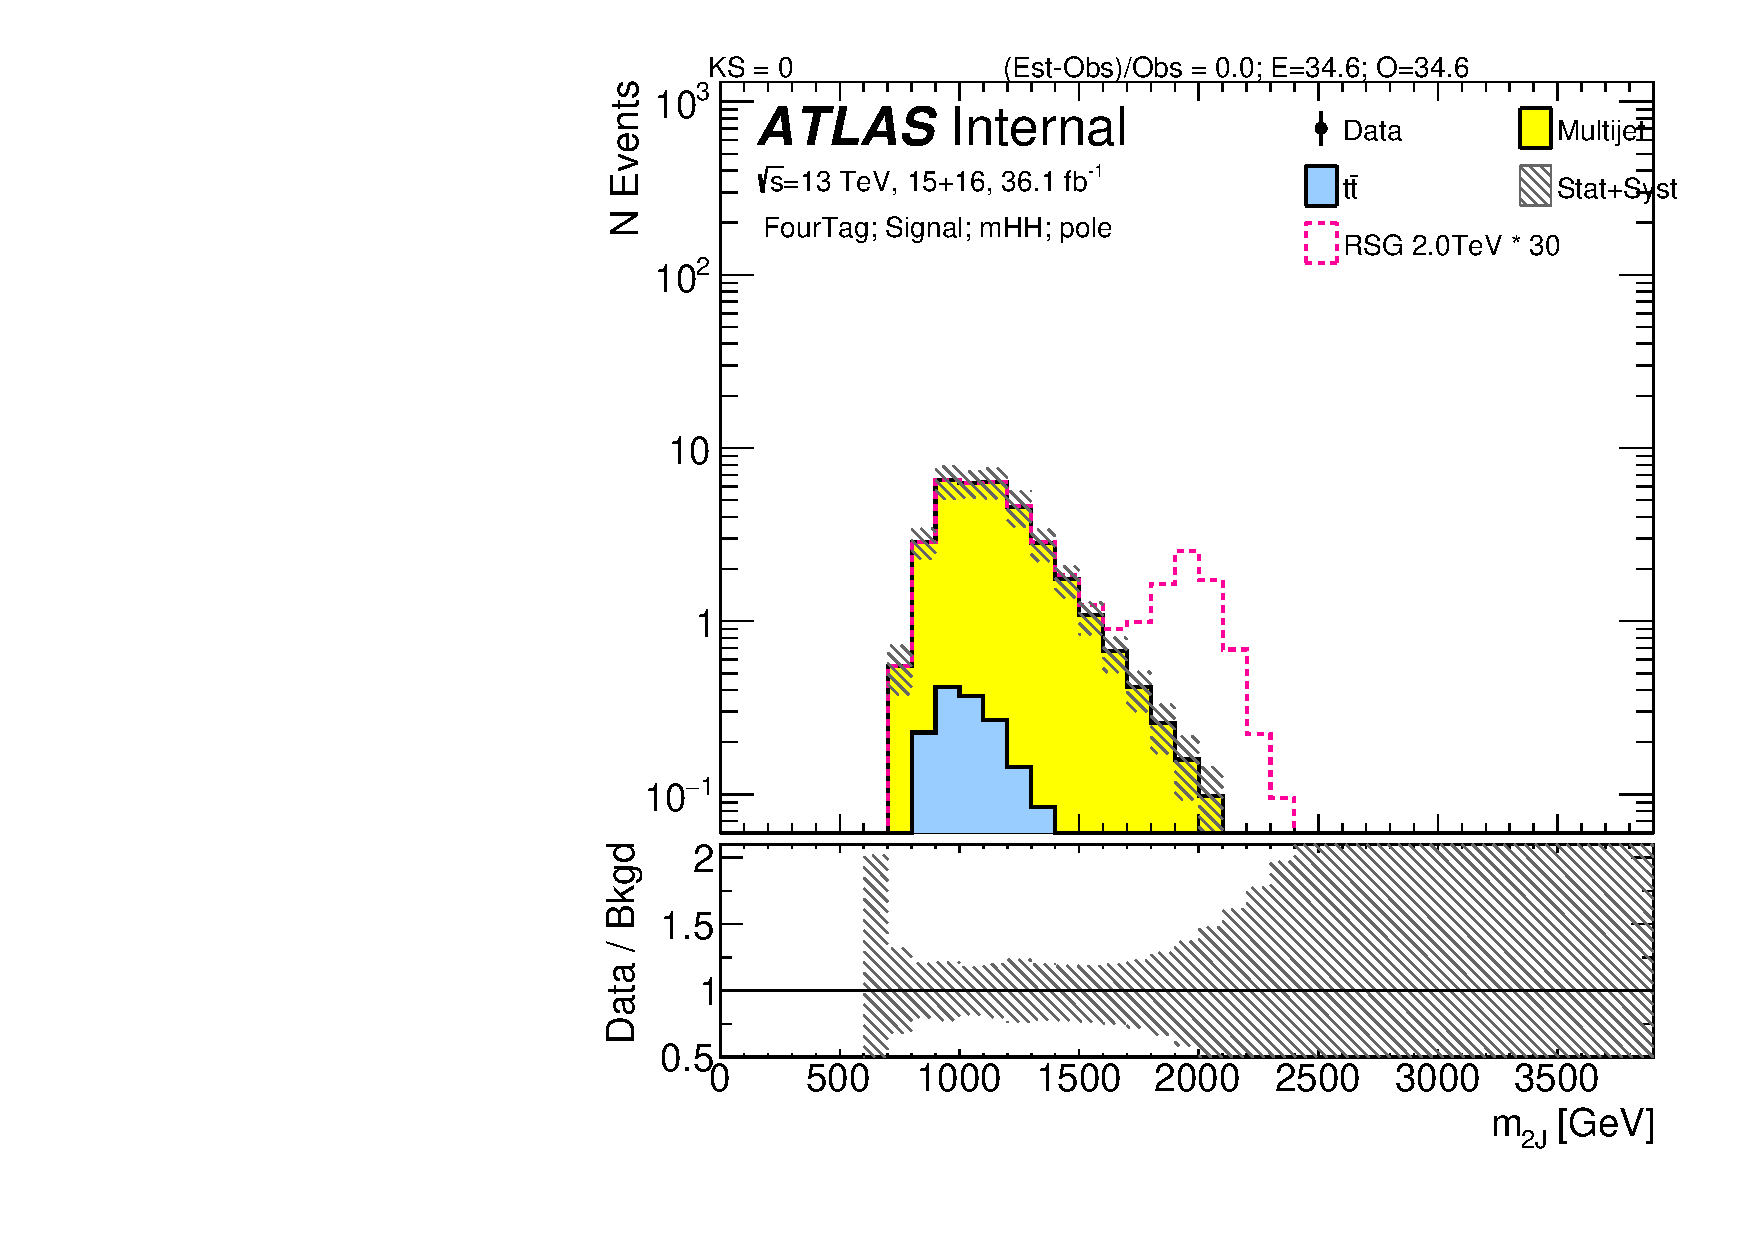
\includegraphics[width=0.48\textwidth,angle=-90]{figures/boosted/Signal_Syst/Moriond_bkg_9_FourTag_Signal_mHH_pole_1_blind.pdf}
\caption{The total background estimation in $4b$ signal region, scaled mJJ, with linear scale on the left and with log scale on the right, along with total uncertainties (stats.$+$systematic) variation up and down.}
\label{fig:FinalBkg_sys-4b-pole}
\end{center}
\end{figure}


\begin{figure}
\begin{center}
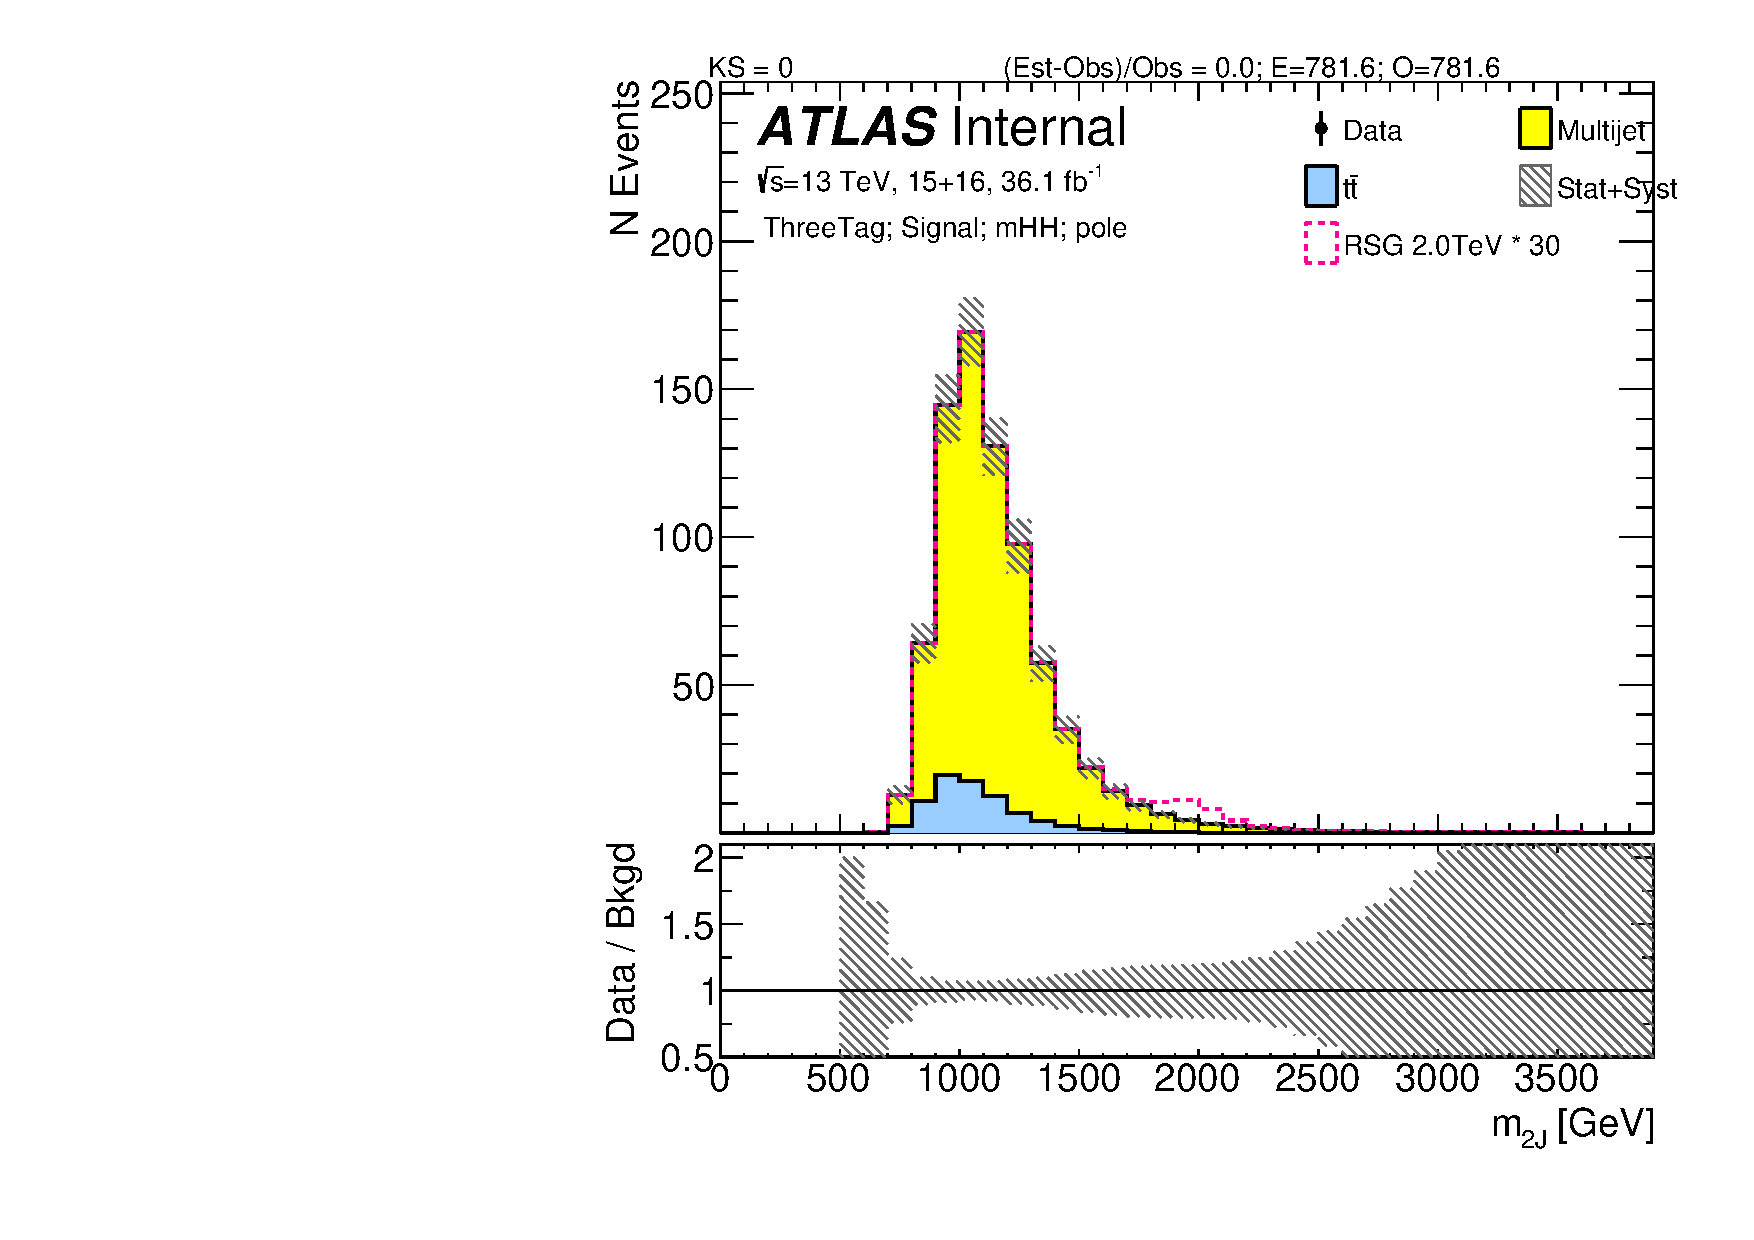
\includegraphics[width=0.48\textwidth,angle=-90]{figures/boosted/Signal_Syst/Moriond_bkg_9_ThreeTag_Signal_mHH_pole_blind.pdf}
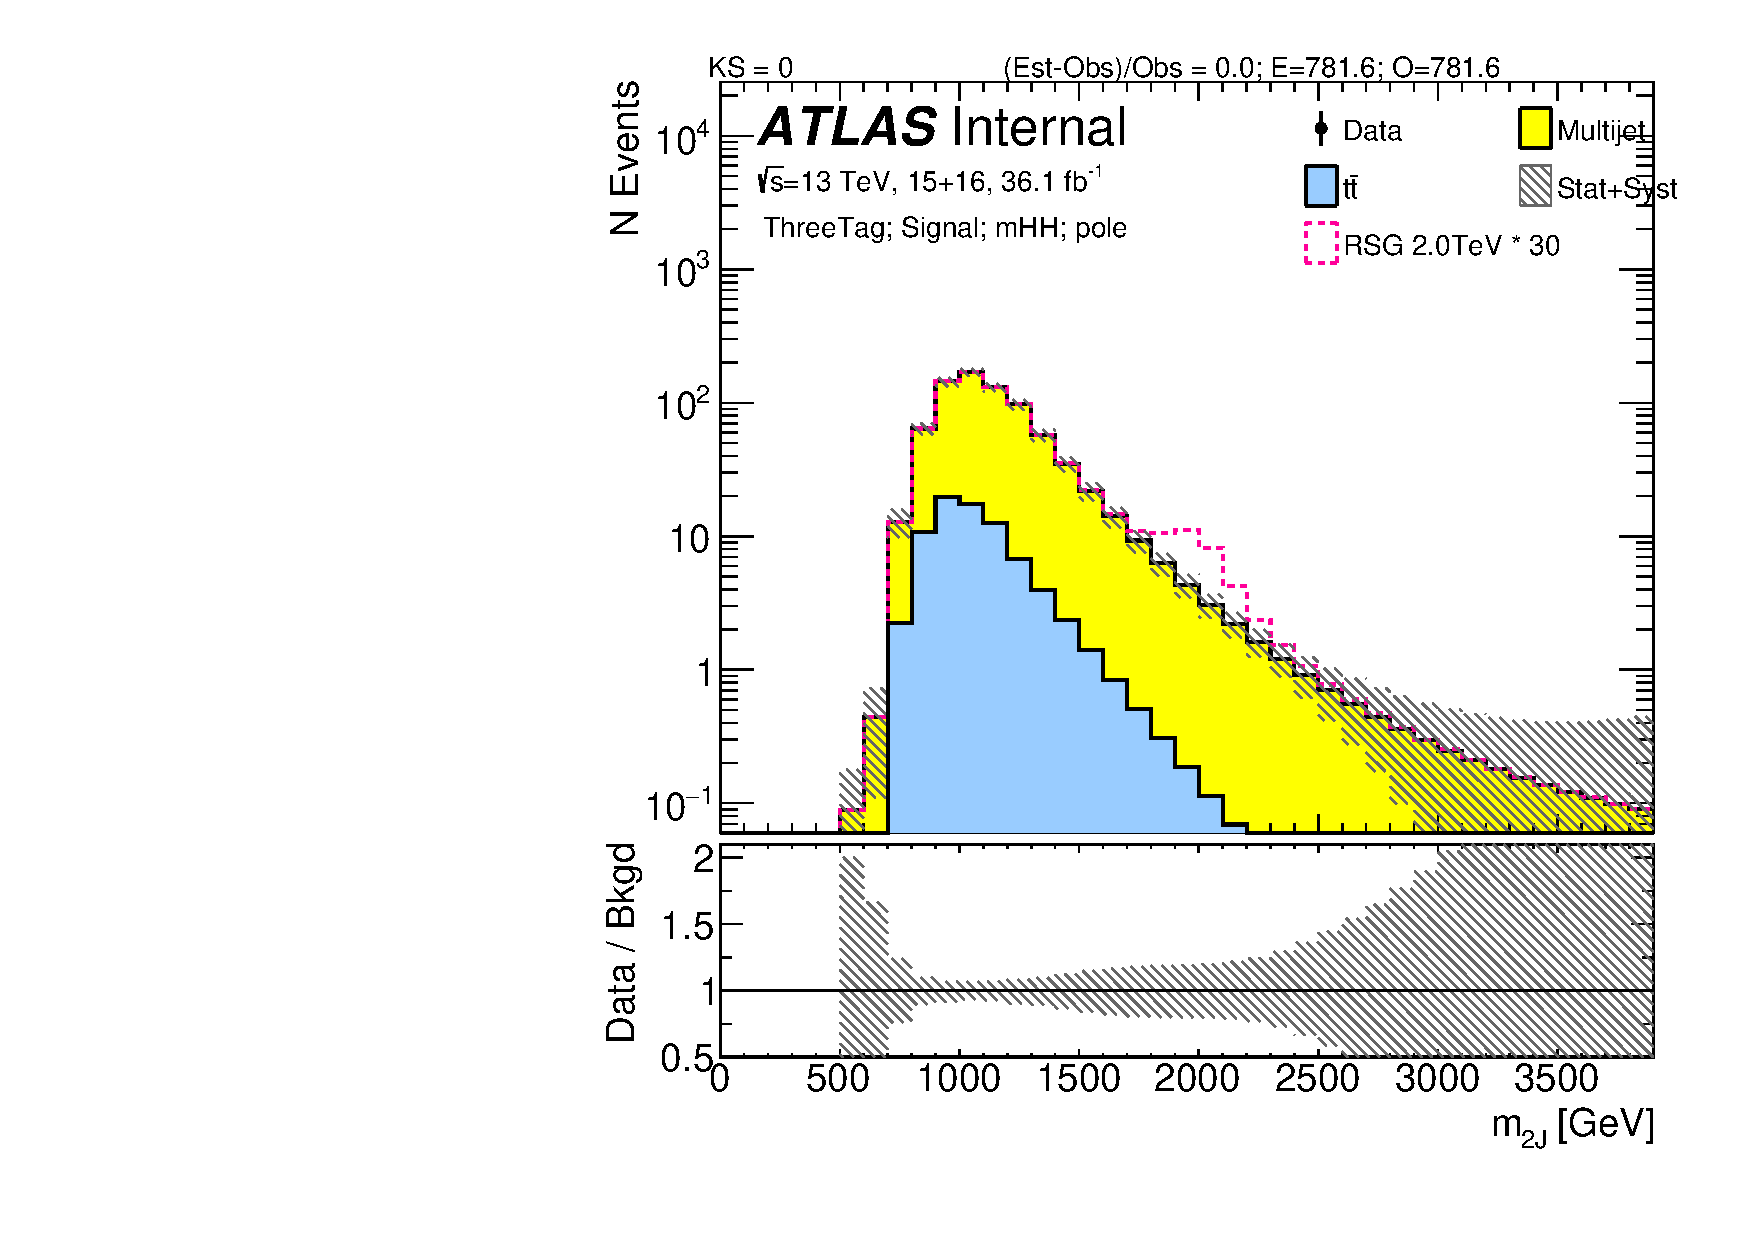
\includegraphics[width=0.48\textwidth,angle=-90]{figures/boosted/Signal_Syst/Moriond_bkg_9_ThreeTag_Signal_mHH_pole_1_blind.pdf}
\caption{The total background estimation in $3b$ signal region, scaled mJJ, with linear scale on the left and with log scale on the right, along with total uncertainties (stats.$+$systematic) variation up and down.}
\label{fig:FinalBkg_sys-3b-pole}
\end{center}
\end{figure}


\begin{figure}
\begin{center}
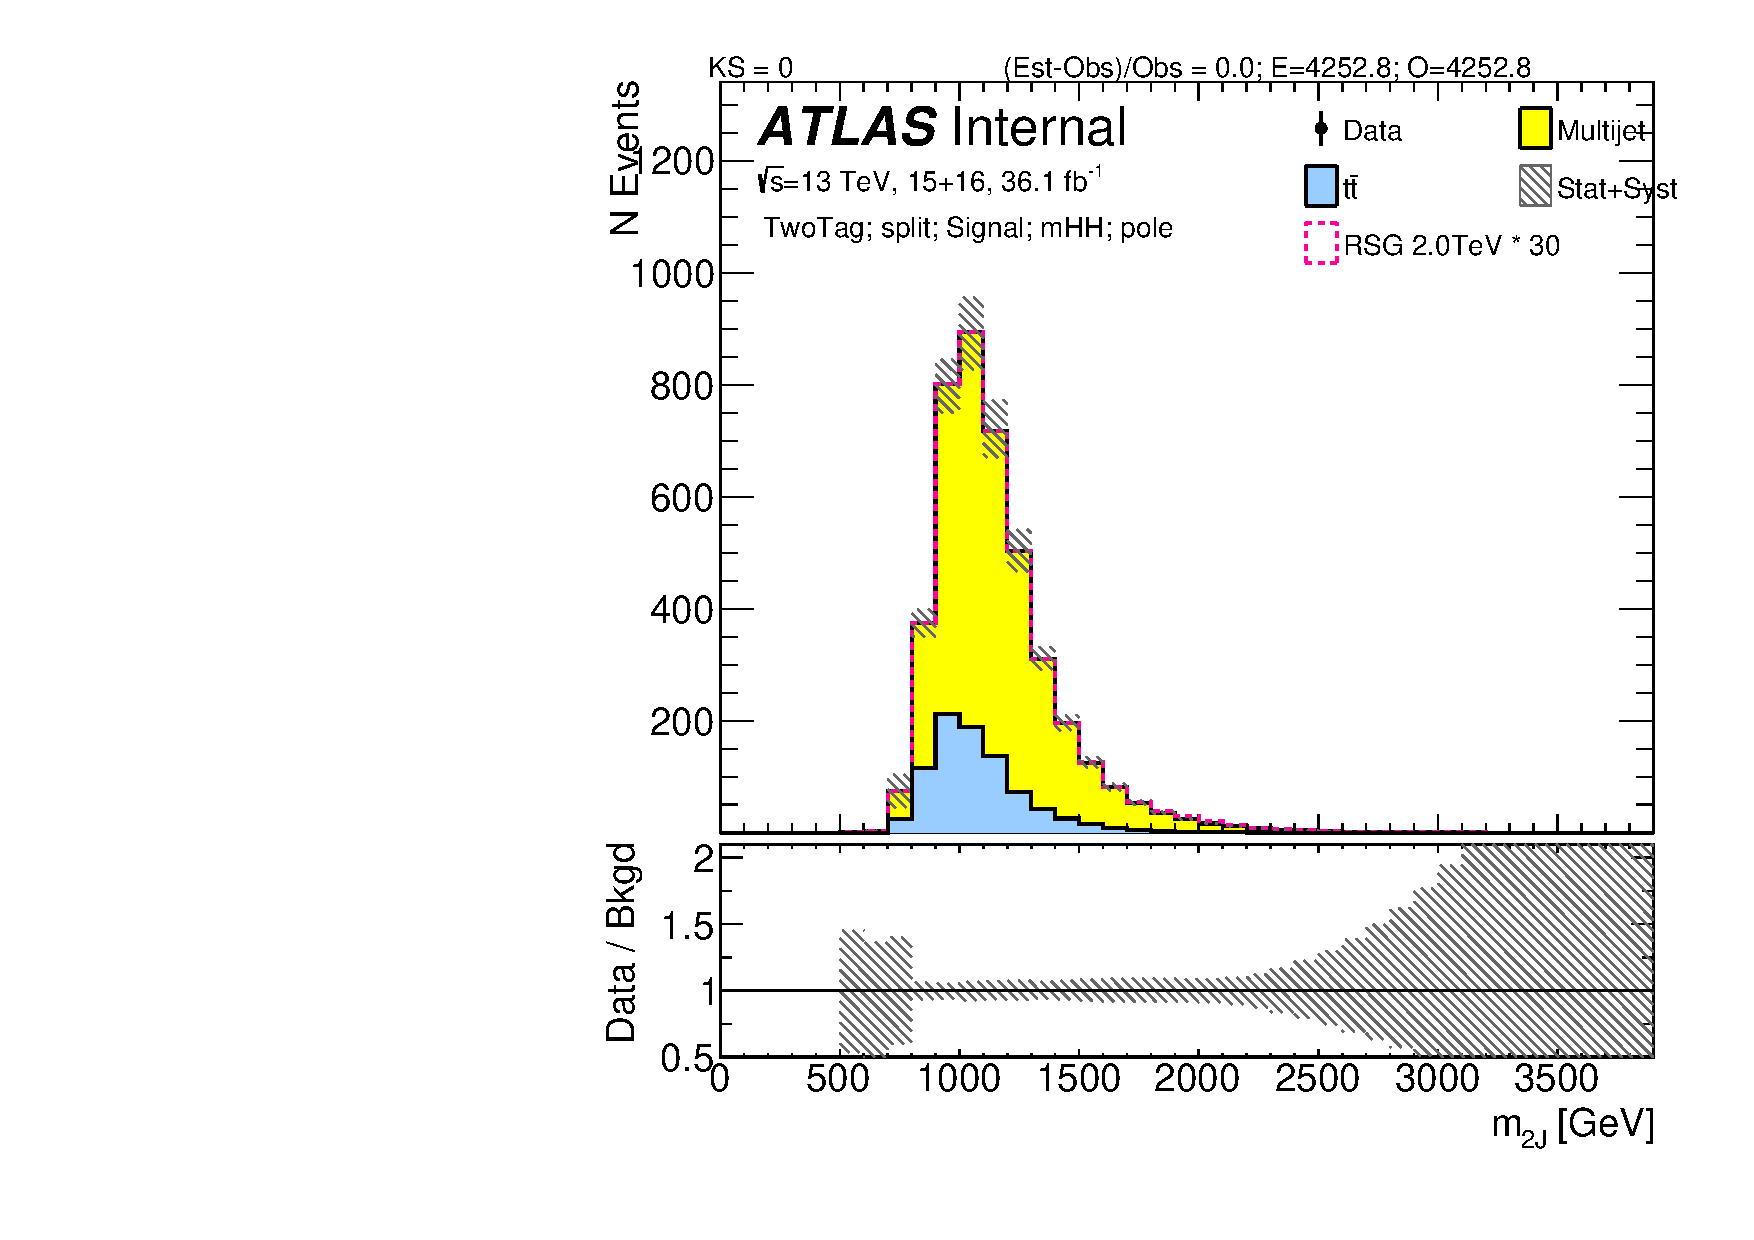
\includegraphics[width=0.48\textwidth,angle=-90]{figures/boosted/Signal_Syst/Moriond_bkg_9_TwoTag_split_Signal_mHH_pole_blind.pdf}
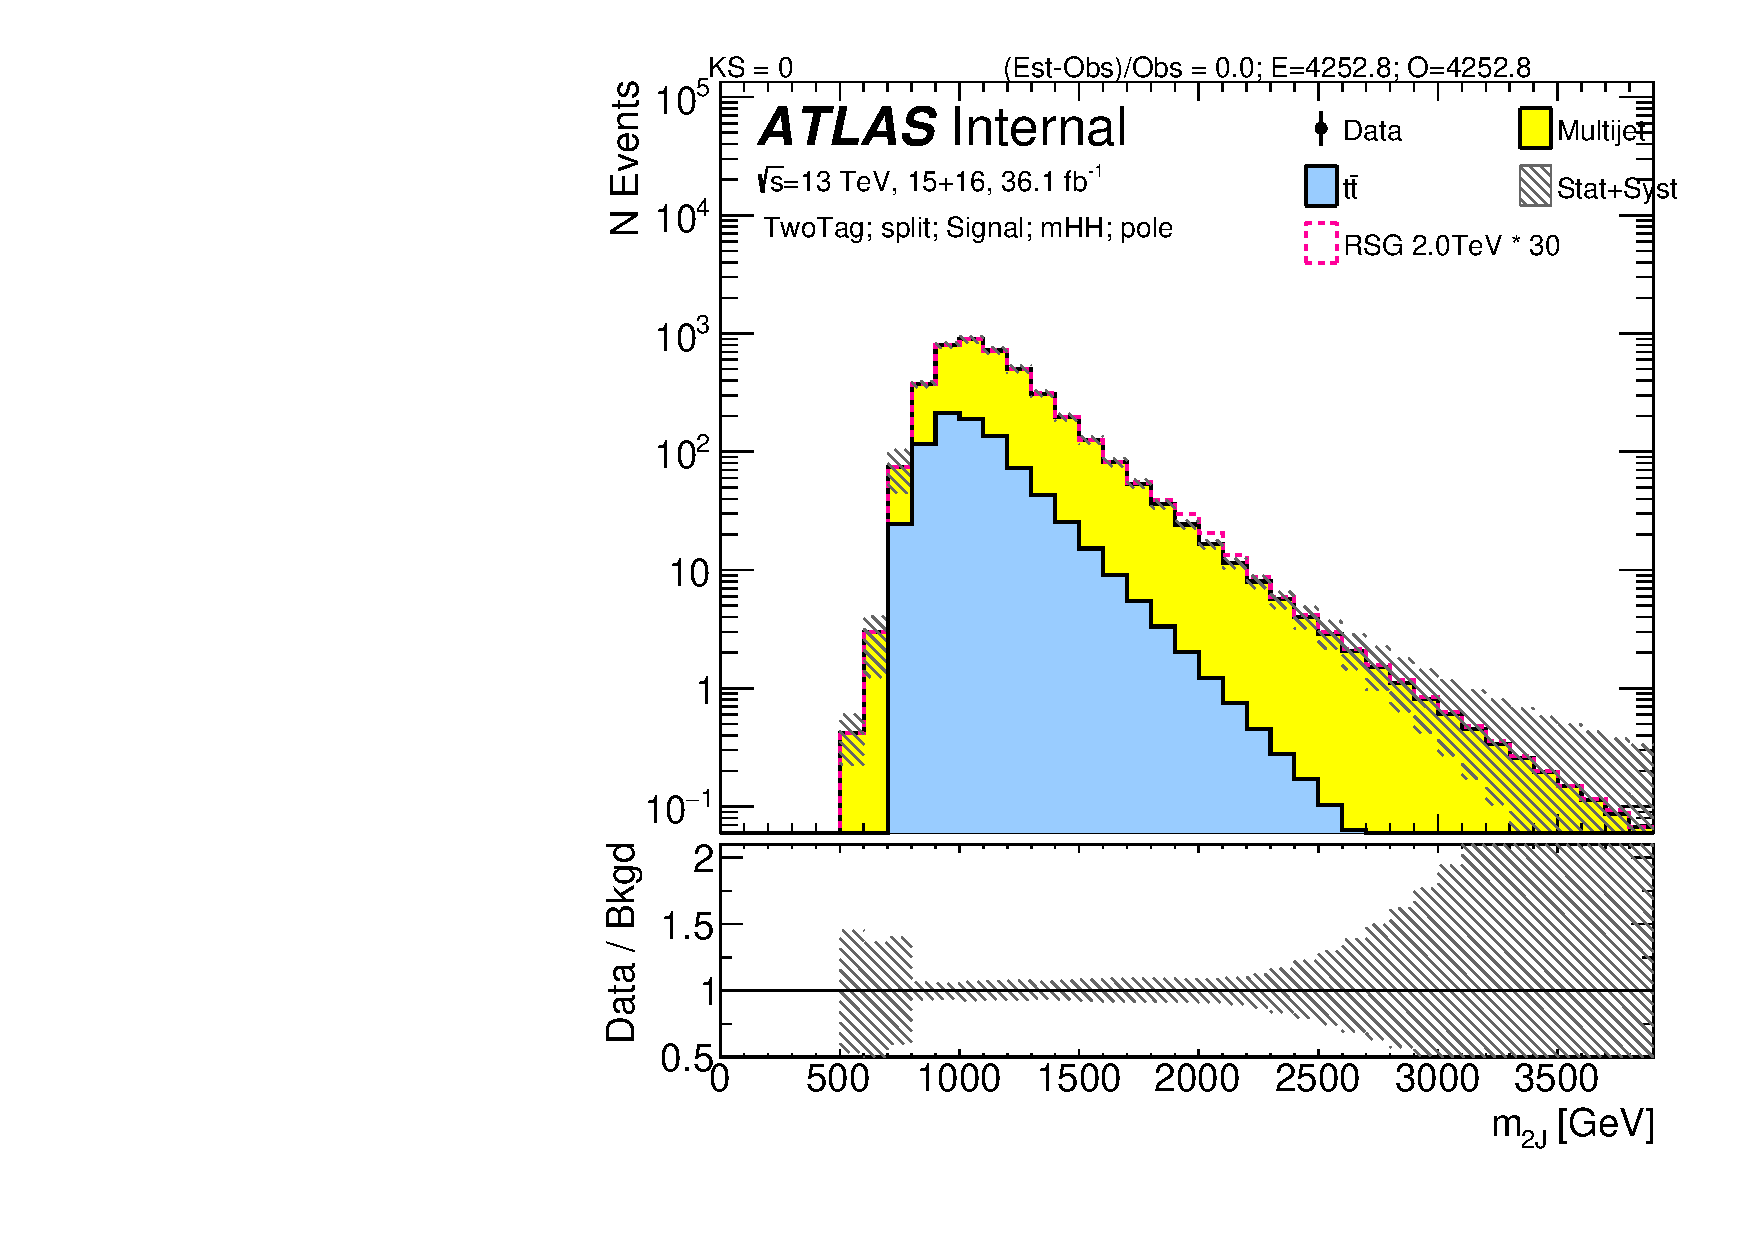
\includegraphics[width=0.48\textwidth,angle=-90]{figures/boosted/Signal_Syst/Moriond_bkg_9_TwoTag_split_Signal_mHH_pole_1_blind.pdf}
\caption{The total background estimation in $2bs$ signal region, scaled mJJ, with linear scale on the left and with log scale on the right, along with total uncertainties (stats.$+$systematic) variation up and down.}
\label{fig:FinalBkg_sys-2b-pole}
\end{center}
\end{figure}


%%%%%%%%%%%%%%%%%%%%%%%%%%%%%%%%%%%%%%%%%%%%%%%%%%%%%%%%%%%%%%%%%%%%%%%
%%%%%%%%%%%%%%%%%%%%%%%%%%%%%%%%%%%%%%%%%%%%%%%%%%%%%%%%%%%%%%%%%%%%%%%